\chapter{Machinelles Lernen}

Der Themenbereich des \keyword{Machinellen Lernens} beschäftigt sich mit Algorithmen und mathematischen Modellen, welche von selber lernen, Probleme zu loesen.
Hierbei wird nicht explizit einprogrammiert, wie das Modell das Problem zu loesen
hat, stattdessen wird das Modell trainiert, optimiert sich von selbst und findet selber
einen Weg, das Problem zu loesen.
Die Grundidee dabei ist, dass man Daten erfasst, generiert oder misst, welche
analysiert werden sollen. Innerhalb dieser Daten existieren gewisse
Gesetzmaessigkeiten und Muster. Diese Muster sollen vom Modell
erkannt werden und verallgemeinert werden. Nach dem erfolgreichen Lernen,
kann das Modell Vorhersagen fuer neuen Daten machen.
\para{}
Man unterscheidet zwischen zwei Arten von Maschinellem Lernen.
\begin{itemize}
\item{
    \keyword{Ueberwachtes Lernen} (engl.:\ supervised learning) ist ein
    Lernverfahren, bei welchem die Daten aus zwei Teilen bestehen, aus Inputs und
    Outputs. Man bezeichnet dabei die Outputs als Labels. Die Aufgabe des Modells
    ist es eine \keyword{Korrelation} zwischen den Inputs und den Labels zu
    erlernen und so ihre Beziehung zueinander zu verstehen.
    Anhand der Informationen, welche in den Inputs enthalten
    sind, sind dann die Labels vorherzusagen. Man gleicht dann die
    vorhergesagten Labels des Modells mit den wahren Labels ab (man
    ``ueberwacht'' sie) und bewertet so die Faehigkeiten des Modells..
    \para{}
    Voraussetztung dafuer ist, dass die Daten eben ``gelabelt'' sein muessen.
    Man muss schon im vorhinein Daten haben, bei welchen man die gewuenschten
    Labels hat. Natuerlich muss auch die erwaehnte Korrelation bestehen. Falls
    kein Zusammenhang zwischen den Inputs und den Outputs besteht, kann das
    Modell auch keine Vorhersagen machen und so auch nichts erlernen.
  }
\item{
    \keyword{Unueberwachtes Lernen} (engl.:\ unsupervised learning) ist ein anderes
    Lernverfahren, bei welchem eben diese Labels nicht vorhanden sind. Dem
    Modell stehen nur die Inputdaten zur Verfuegung. Diese werden ebenfalls analysiert
    und das Modell soll Muster herausextrahieren, welche sich von sonstigem
    zuefaelligen Rauschen unterscheiden.
  }
\end{itemize}

Der Grossteil der Modelle des Maschinellen Lernens benutzen ueberwachtes
Lernen, da es auch deutlich mehr Anwendungsmoeglichkeiten besitzt. Es gibt nur wenige Arten von
unueberwachtem Lernen, dazu gehoeren: Hauptkomponentenanalysen und Generative
Adversial Networks. Aus diesem Grund, werden wir im folgenden uns grundsaetzlich
mit ueberwachtem Lernen beschaeftigen.
\para{}
\cite{wiki:supervised_learning}
\cite{wiki:unsupervised_learning}

\section{Allgemeine Begriffe}

\subsection{Daten}

Um ein Modell zu trainieren, braucht man Daten. Diese Daten bestehen immer aus
\keyword{Inputs} und \keyword{Outputs}. Man unterscheidet hierbei zwischen zwei Arten
von Outputs. Die \keyword{Labels} sind die erwarteten Outputs, welche die
gewueschten Zielwerte sind. Die \keyword{Vorhersagen} sind die Outputs, welche
das Modell produziert und hoffentlich moeglichst genau mit den Labels
uebereinstimmen.
\para{}
Diese Daten fuer das Training kommen in der Form eines \keyword{Trainingsdatensatzes} $\set{X}$.
Dabei handelt es sich um eine Menge von \keyword{Samples},
welche jeweils aus Inputs und Labels bestehen.
Die Inputs werden in einem Vektor
\[ \vec{x} = \trans{\begin{pmatrix} x_1 & x_2 & \cdots & x_m \end{pmatrix}} \]
und die Labels in einem Vektor
\[ \vec{\hat{y}} = \trans{\begin{pmatrix} \hat{y}_1 & \hat{y_2} & \cdots & \hat{y}_n \end{pmatrix}} \]
zusammengefasst.Somit ist ein Trainingssample nichts anderes als ein Paar
$(\vec{x}_i,\vec{\hat{y}}_i)$ eines Inputsvektor $\vec{x}$ und eines Labelvektor
$\vec{\hat{y}}$.
Die Vorhersagen werden ebenfalls in einem Vektor
\[\vec{y} = \trans{\begin{pmatrix} y_1 \quad y_2 \quad \cdots \quad y_n \end{pmatrix}} \]
zusammengefasst.
\para{}
Die Inputs beinhalten sogennanten \keyword{Features} (deutsch: Merkmale). Sie
zeichnen die Inputs aus und umfassen ihren ganzen Informationsgehalt.
Der Algorithmus soll
anhand dieser Features seine Vorhersagen machen.
Diese Vorhersagen werden dann mit den Labels abgeglichen und so bewertet.
Anhand der Bewertungen wird dann eine Optimierung des Modells vorgenommen.
Unter korrekten Bedingungen (kein Overfitting) findet kein Auswendiglernen der Trainingsdaten statt,
sondern ein Generalisieren des Zusammenhangs anhand von Mustern und Gesetzmassigkeiten.
\para{}
Um eine endgueltige Bewertung des Modells durchzufuehren, wird ein Testdatensatz
$\set{T}$, welcher nicht Teil des Trainingsdatensatz ist, genutzt, um Vorhersagen zu machen.
Dies garantiert, dass kein Auswendiglernen moeglich ist.
\para{}
BEISPIEL


\subsection{Modelle}
Ein \keyword{Modell} ist eine mathematische Funktion $\mathit{h}\colon \set{R}^m
\to \set{R}^n$, Hypothesenfunktion gennant, welche die Inputs auf die Outputs abbildet $\vec{y}=\mathit{h}(\vec{x})$.
Man kann diese Funktion gewissermassen als die Hypothese, welche das Modell bezueglich der Beziehung zwischen
den Inputs und den Labels aufgestellt hat, betrachten.
Diese Modelle koennen verwendet werden um vorallem entweder
Klassifizierungsprobleme oder Regressionsprobleme zu loesen. Falls es sich um
letzteres handelt, spricht man von einem Regressionsmodell. Ein solches
Regressionsproblem werden wir in dieser Arbeit loesen.
\para{}
Das Verhalten eines Modells wird bestimmt durch seine \keyword{Modellparameter}
$\param_1, \param_2,\ldots,\param_k$. Sie bestimmen, wie die Hypothese des Modells lautet.
Das Ziel ist es, die Modellparameter so einzustellen, dass die Vorhersagen
$\vec{y}$ des Modells besser mit den Labels $\vec{\hat{y}}$ der Trainingsdaten uebereinstimmen.
Dies wird iterativ gemacht, indem immer wieder leichte Anpassungen an den
Parametern vorgenommen werden, bis das Modell die gewuenschten Resultate liefert.
\para{}
Neben den gelernten Parametern, gibt es auch noch sogenannte \keyword{Hyperparameter}.
Diese koennen nicht erlernt werden, sondern muessen manuell vor dem Training gewaehlt werden und koennen den Lernvorgang erheblich beeinflussen.
Dies bedeutet, dass man ausprobieren muss, welche Werte fuer die Hyperparameter
die besten Resultate liefern.
\para{}
Das wohl einfachste Regressionsmodell ist eine Regressionsgerade. Diese ist
angemessen, falls ein einfacher linearen Zusammenhang der Form $y=\param_1x +
\param_0$ zwischen den Features und den Labels besteht.
Nun muessten nur noch $\param_0$ und $\param_1$ bestimmt werden.
BEISPIELMODELL AUTO
\para{}
Fuer Machine Learning haben sich gewisse Modelle besonders gut etabliert,
darunter waeren: Support Vector Machines, Evolutionäre Algorithmen, und Künstliche Neuronale Netze.
Diese Arbeit wird sich vorwiegend mit Neuronalen Netzen auseinandersetzen.
\\
\begin{figure}[h!]
  \centering


  \caption{Schema eines Modells}
\end{figure}

\section{Training}
\subsection{Verlust- und Kostenfunktionen}
Einsicht ist der erste Schritt zur Besserung. Das gilt auch beim Machine Learning, deshalb muss beim Training zuerst die Genauigkeit des Modells bewertet werden.
Dies wird mithilfe von sogennaten Kostenfunktionen bzw. Verlustfunktionen erreicht.
\para{}
Eine \keyword{Verlustfunktion} $L(y,\hat{y})$ soll ein Mass fuer die
Abweichung der Vorhersage $y$ von dem Label $\hat{y}$ sein.
Aus ihr bildet man die \keyword{Kostenfunktion} $C(\vec{y},\vec{\hat{y}})$, indem man die
Verluste der einzelnen Ouputs aufsummiert. Somit erhaelt man die Kosten
einer gesamten Vorhersage mit $m$ Outputs (siehe Gl. (\ref{eq:errorfunc})). Bei
gewissen Kostenfunktionen gibt es keine Verlustfunktion, da sie nicht auf die
einzelnen Outputpaare aufgebrochen werden kann. \\
Der Fehler $\bar{C}(\set{X})$ des gesamten Trainingsdatensatzes $\set{X}$, der
Groesse $p$, ergibt sich aus dem arithmetischen Mittel der einzelnen Kosten der
Vorhersagen (siehe Gl. (\ref{eq:meanerrorfunc})).
\\
\begin{minipage}[h!]{0.5\textwidth}
  \begin{equation}\label{eq:errorfunc}
    C \left(\vec{y},\vec{\hat{y}} \right) = \ds\sum_{i=1}^{m} L(y_i, \hat{y}_i)
  \end{equation}
\end{minipage}
\begin{minipage}[h!]{0.5\textwidth}
  \begin{equation}\label{eq:meanerrorfunc}
    \bar{C}(\set{X}) = \frac{1}{p}\ds\sum_{j=1}^{p} C\left(\vec{y}_j,\vec{\hat{y}}_j\right)
  \end{equation}
\end{minipage}
\para{}
Eine eine Kostenfunktion $C$ sollte folgende Eigenschaften aufweisen:
\begin{itemize}
\item{$C$ ist minimal, wenn $\vec{y} = \vec{\hat{y}}$}
\item{$C$ waechst mit $|\vec{y} - \vec{\hat{y}}|$}
\item{$C$ ist nach jedem $y_n$ partiell differenzierbar (erklaert in Sektion (\ref{ref:partielle_ableitungen}))}
\end{itemize}
\para{}

\cite{Nielsen}

\subsubsection{Mittlere quadratische Abweichung}
Die bekannteste Kostenfunktion ist die ``Mittlere quadratische Abweichung''.
(engl.:\ mean squared error). Sie ist definiert als das arithmetische Mittel
aller quadrierten Differenzen zwischen den Vorhersagen und Labels.
Zusaetzlich halbiert man noch das arithmetische Mittel, damit bei der Ableitung der Faktor
$2$ wegfaellt. Sie hat keine entsprechene Verlustfunktion, da man so das
arithemtische Mittel nicht schreiben kann.
\\
Die Kostenfunktion kann mithilfe einer Summe berechnen werden, oder in
diesem Fall mithilfe einer Vektorsubtraktion Vorhersagen $\vec{y}$ von den Labels $\vec{\hat{y}}$.
\\
\begin{equation}\label{eq:MSE}
  C_{MSE} = \frac{1}{2n}\sum_{i=1}^{n}{(\hat{y}_i - y_i)}^2 = \frac{1}{2n}{(\vec{\hat{y}} - \vec{y})}^2
\end{equation}
\\
Sie erfuellt alle Anforderungen an eine Kostenfunktion:
\begin{itemize}
\item{Ihr Funktionwert ist 0 und minimal fuer $\vec{y} = \vec{\hat{y}}$}
\item{Sie ist proportional zu ${(\vec{\hat{y}}-\vec{y})}^2$}
\item{Ihre partielle Ableitung nach einem $y_i$ lautet: $C_{MSE}'=\frac{1}{n}(y_i-\hat{y_i})$}
\end{itemize}


\subsubsection{Cross-entropy}


\subsection{Gradientenverfahren}\label{sec:gradientenverfahren}
Um ein Modell nun zu trainieren, muss man verstehen, dass es sich um ein Optimierungsproblem handelt.
Das Modell ist am besten, also macht die besten Vorraussagen, wenn die
Funktionswerte der Kostenfunktion am kleinsten sind.
Deshalb muss diese Kostenfunktion $C$ minimiert werden.
Hierbei muss die Funktion $C$ nicht mehr in Abhaengigkeit der Inputs und Outputs betrachtet
werden, sondern als Funktion der Modellparameter
$C(\param_1, \param_2, \ldots, \param_k)$, denn diese sollen angepasst werden,
um das Modell zu verbessern.
Fuer diese Optimiertung wird das sogennante \keyword{Gradientenverfahren} (engl.: Gradient descent) verwendet.
\footnote{%
  Im Gymnasium wird beigebracht die lokalen Extrema (inklusive lokalen Minimas) zu
  bestimmen, indem die erste Ableitung $f'$ gebildet wird und gleich null gesetzt
  wird.Dies ist hier nicht moeglich, da die Funktion
  $C'(\param_1,\param_2,\ldots,\param_n)$ deutlich zu komplex ist, um die
  Nullstellen analytisch zu bestimmen. Deshalb wird das Gradientenverfahren
  verwendet.
}
\para{}
Allgemein koennen mithilfe des Gradientenverfahrens Funkionen $f(x_1, x_2, \ldots, x_n)$ vom Typ $\set{R}^n \to \set{R}$ (wie z.B. die Fehlerfunktion) minimiert werden.
Dies geschieht, indem ein Startpunkt (Ortsvektor) $\vec{p}_0$, dessen
Komponenten den Input von $f(\vec{p}_0)$ darstellen, gewaehlt wird.
Nun werden iterativ neue Punkte $\vec{p}_t$ gesucht, welche immer naeher beim lokalen Minimun liegen, also Punkte, die den Funktionswert $f(\vec{p}_t)$ immer kleiner werden lassen.
Dies wird durchgeführt, bis der Punkt genuegend nahe beim lokalen Minimun ist.
\para{}
Dafuer muss ein Vektor $\vec{b}_t$ bestimmt werden, welcher auf den Punkt $\vec{p}_t$ addiert einen neuen Punkt $\vec{p}_{t+1}$ bildet,
bei dem der Funktionswert $f(\vec{p}_{t+1})$ kleiner ist als der von $f(\vec{p}_t)$.
Dies geschieht am effizientesten, wenn $\vec{b}_t$ in die Richtung der staerksten Funktionswertabnahme zeigt.

Hierzu braucht man den sogennanten \keyword{Gradient} $\vecf{\nabla}$, wofür man wiederum partielle Ableitungen braucht.
\para{}
\begin{defbox}{Partielle Ableitungen}\label{ref:partielle_ableitungen}
  Partielle Ableitungen sind eine Erweiterung der ``normalen'' Ableitungen auf
  multidimensionale Funktionen $f(\vec{x}) = f(x_1,\ldots,x_n): \set{R}^n \to \set{R}$.
  Man leitet dabei nur nach einem Argument $x_i$ ab und betrachtet die restlichen Argumente als Konstanten.
  Es gelten die gleichen Ableitungsregeln wie bei der nicht-partiellen Ableitung.
  Die partielle Ableitung einer Funktion $f(x_1,\ldots,x_n)$ bezueglich einer
  Variable $x_i$ in einem Punkt $\vec{a} = \trans{\begin{pmatrix} a_1 & \cdots & a_n \end{pmatrix}}$
  ist analog zur normalen Ableitung folgendermassen definiert:
  \begin{equation*}
    \partderiv{f}{x_i}(\vec{a}) \coloneqq \lim_{h \to 0} \frac{f(a_1,\ldots,a_i + h,\ldots,a_n)-f(a_1,\ldots,a_i,\ldots,a_n)}{h}
  \end{equation*}
  Geometrisch ist dies die Steigung der Tangente an die Funktion $f$ im Punkt
  $\vec{a}$. Die Tangente liegt in der Richtung der Achse des Parametern $x_i$, nach dem man ableitet.
\end{defbox}
\\
\begin{defbox}{Gradient}
  Der Gradient $\vecf{\nabla}$ ist ein Differentialoperator, den man auf eine
  Funktion $f(\vec{x}) = f(x_1,\ldots,x_n): \set{R}^n \to \set{R}$ anwendet kann, welcher ein Skalarfeld auf ein Vektorfeld (das sogennante Gradientenfeld) abbildet.\\
  Um den Gradienten $\vecf{\nabla}f$ der Funktion $f$ zu bilden, fasst man alle partiellen Ableitungen der Funktion $f$, nach jedem
  Argument $x_i$, in einem Vektor zusammen. Meistens bestimmt man den Gradienten
  $\vecf{\nabla} f(\vec{p})$ in einem spezifischen Punkt $\vec{p} =
  \trans{\begin{pmatrix} p_1 & \cdots & p_n \end{pmatrix}}$.
  \begin{equation*}
    \vecf{\nabla}_{\vec{x}} f(\vec{p}) = \ds\partderiv{f}{\vec{x}}(\vec{p}) =
    \begin{pmatrix}
      \ds\partderiv{f}{x_1}(\vec{p}) \\
      \vdots \\
      \ds\partderiv{f}{x_n}(\vec{p}) \\
    \end{pmatrix}
  \end{equation*}

  Geometrisch ist der Gradient $\vecf{\nabla}f(\vec{p})$ einer Funktion $f$ in
  einem Punkt $\vec{p}$ dann der Vektor, welcher in die Richtung des steilsten
  Anstiegs von $f$ zeigt. Sein Betrag gibt die Staerke des Anstiegs an.
\end{defbox}
\para{}
\begin{figure}[h!]
  \centering
  \begin{tikzpicture}
    \begin{axis}[
      domain=-2:2,
      view={0}{90},
      axis background/.style={fill=white},
      legend style={cells={align=left},at={(1.2,1)},anchor=east}
      ]
      \addplot3[contour gnuplot={number=9,
        labels=false},thick]
      {exp(0-x^2-y^2)*x};
      \addlegendentry{Isolinien\\ von $f(x_1,x_2)$}
      \addplot3[blue,
      quiver={
        u={exp(0-x^2-y^2)*(1-2*x^2)},
        v={exp(0-x^2-y^2)*(-2*x*y)},
        scale arrows=0.3,
      },
      -stealth,samples=15]
      {exp(0-x^2-y^2)*x};
      \addlegendentry{$\vecf{\nabla}f$}
    \end{axis}
  \end{tikzpicture}
  \caption{ein Skalarfeld als Konturdiagramm mit zugehoerigem Gradientenfeld}
\end{figure}
\para{}
Da der Gradient in die Richtung des steilsten Anstiegs zeigt, sollte der Vektor
$\vec{b}_t$ gerade in die entgegengesetze Richtung zeigen. Also sollte er in die Richtung des negierten Gradienten der Funktion $f$ im Punkt $\vec{p}_t$ zeigen.
Also kann jetzt das iterative Annaehern an das lokale Minimum folgendermassen beschrieben
werden (wobei $\eta$ eine spaeter erklaerte Schrittgroesse darstellt).
\\
\begin{equation}\label{eq:gradientdescent}
  \vec{p}_{t+1} = \vec{p}_t - \eta \cdot \vecf{\nabla} \mathit{f}(\vec{p}_t)
\end{equation}
\\

\ifcp%
\begin{figure}[h!]
  \centering
  \begin{tikzpicture}
    \begin{axis}[
      % hide axis,
      xticklabels={,,},
      yticklabels={,,},
      zticklabels={,,},
      xlabel=$x_1$,
      ylabel=$x_2$,
      colormap/cool,
      legend style={at={(1,1.2)},anchor=north east},
      reverse legend
      ]
      \addplot3[domain=-1:1,orange, quiver={u={(1+exp(-(x^2+y^2)))^(-2)*exp(-(x^2+y^2))*(-2*x)}, v={(1+exp(-(x^2+y^2)))^(-2)*exp(-(x^2+y^2))*(-2*y)}, scale arrows=0.4}, -stealth,samples=10] {0.5};
      \addlegendentry{$-\vecf{\nabla}_{\vec{x}}f$}

      \addplot3[
      mesh,
      samples=50,
      domain=-1:1,
      ]
      {1/(1+exp(-(x^2+y^2)))};
      \addlegendentry{$f(x_1,x_2)$}

      \coordinate (ballpos) at (axis cs:-0.8,0.8,{1/(1+exp(-((-0.8)^2+(0.8)^2)))});
      \coordinate (bottom) at (axis cs:0,0,0.5);
      \draw[red,very thick,->,>=latex] (ballpos) -- ($(ballpos)!0.3!(bottom)$);
      \shade [ball color=yellow] (ballpos) circle (0.25cm);
    \end{axis}
  \end{tikzpicture}
  \caption{Visualisierung des Gradientenabstiegs: ein Ball rollt das
    Gradientenfeld hinab in das lokale Minimum.}
\end{figure}
\fi%

Waehrend des Gradientenverfahren konvergiert der Punkt $\vec{p}_t$ zu einem
beliebigen \textit{lokalen} Minimum, abhängig davon wie der Startpunkt
$\vec{p}_0$ gewaehlt wurde.
Wie man diesen Startpunkt zu waehlen hat, wird in Sektion
(\ref{sec:parameter_initalisieren}) erlauetert.
Da dieser meist zufaellig bestimmt wird, ist es eine Glückssache ein sehr niedriges Minimum zu finden.
\para{}
Die sogennante \keyword{Lernrate} $\eta$ aus Gleichung (\ref{eq:gradientdescent}) ist ein Hyperparameter.
Sie ist ein positiver Proportionalitatsfaktor, welcher die Schrittgroesse des
Gradientenabstiegs bestimmt. Sie muss je nach zu minimierender Funktion anders gewaehlt werden.
Dabei hilft nur Ausprobieren. Falls $\eta$ nicht gut gewaehlt wurde, gibt es Probleme beim Training:
\begin{itemize}
\item{Falls $\eta$ zu klein ist, verlaueft das Trainings unnoetig langsam und braucht sehr lange.
    Ausserdem kann es passieren, dass man bei einem hohen lokalen Minimum stecken bleibt.}

\item{Falls $\eta$ zu gross ist, kann es passiert, dass man ueber das lokale
    Minimum hinaus schiesst und somit nur darum herum springt.}
\end{itemize}

\begin{figure}[h!]
  \centering
  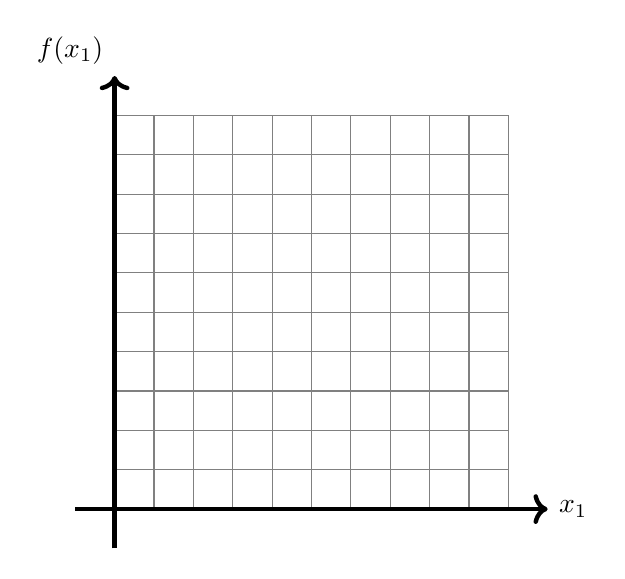
\begin{tikzpicture}
    \draw[gray] (0,0) grid[step=0.5cm] (5,5);
    \draw[ultra thick,black,->] (-0.5,0) -- (5.5,0) node[right] {$x_1$};
    \draw[ultra thick,black,->] (0,-0.5) -- (0,5.5) node [above left] {$f(x_1)$};
  \end{tikzpicture}
  \caption{Visualisierung verschiedener Lernraten}
\end{figure}

\para{}
\cite{Nielsen}

\subsection{Stochastisches Gradientenverfahren fuer Machine Learning}
Wie oben erklaert, wird fuer das Trainieren eines Modells das Gradientenverfahren benutzt.
Konkret wird die Kostenfunktion $C(\vec{y},\vec{\hat{y}}\ |\ \param_0,\ldots,\param_n)$
($\param_i$ sind die Modellparameter, $\vec{y}$ die Vorhersagen und $\vec{\hat{y}}$
die Labels) minimiert, indem die Parameter angepasst werden. Dadurch macht das Modell immer bessere Vorhersagen.
Fuer nur eine Iteration des Gradientenverfahren, muesste man den Gradienten fuer den
\textit{gesamten} Trainingsdatensatz berechnen.
Dies waere zwar ein exakter Prozess, aber ein extrem langsamer zugleich.
Bei grossen Datensaetzen wuerde es eine Ewigkeit dauern, bis das Modell nur annahernd guete Vorhersagen machen wuerde.
\para{}
Aus diesem Grund verwendet man eine leicht abgeänderte Variante dieses
Verfahren, naemlich das \keyword{Stochastische Gradientenverfahren} (engl.:
Stochastic Gradient Descent) (SGD).
Hierfuer wird der ``echte'' Gradient des gesamten Datensatzes mit dem Gradienten einiger Trainingssamples approximiert.
Dazu wird der Trainingsdatensatz in sogennante \keyword{Mini-Batches} eingeteilt und der Gradient jeweils pro Mini-Batch berechnet.
Als Konsequenz finden deutlich mehr Iterationen in \textit{einer}
Durchkaemmung der Trainingsdaten statt. Eine solche Durchkaemmung bezeichnet man als
\keyword{Epoche}. Oft wird mehrere Epochen lang trainiert.
Der Gradient eines genug grossen Mini-Batches ist zwar nicht ganz exakt, aber approximiert den Gradieten des gesamten Datensatzen genuegend gut.
Sowohl die Mini-Batch Groesse, wie auch die Anzahl Epochen sind weitere Hyperparameter.
\para{}
Die partiellen Ableitungen der gesamten Trainingsdaten wird mit dem
arithmetischen Mittel der partiellen Ableitungen eines Mini-Batches der Groesse $q$ approximiert.
\\
\begin{equation}\label{eq:minibatch_deriv}
  \partderiv{\bar{C}}{\param_k} \approx \frac{1}{q}\sum_{i=1}^{q} \partderiv{C_i}{\param_k}
\end{equation}
\\
Eine Iteration des Stochastischen Gradientenverfahren wird analog zu Gleichung (\ref{eq:gradientdescent}) folgendermassen durchgefuehrt.
\\
\begin{equation}\label{eq:sgd}
  \param_{k,t+1} = \param_{k,t} - \frac{\eta}{q} \sum_{i=1}^{q} \partderiv{C_i}{\param_{k,t}}
\end{equation}

\cite{Nielsen}

\subsection{Adam Optimizer?}

\section{Trainingsphaenomene}

\subsection{Konvergenz und Divergenz}
\subsection{Underfitting und Overfitting}

% ------------------------------------------------------------

\chapter{Deep Learning und Künstliche Neuronale Netze}
Nun betrachten wir ein spezifisches Modell, welches die wohl besten Resultate
fuer die meisten Problemstellungen des Maschinellen Lernens (Bilderkennung,
Spracherkennung, etc.) liefert. Es handelt sich um das \keyword{Kuenstliche Neuronale Netz} (eng.: Neural Network) kurz KNN.
Der Bereich des Maschinellen Lernens, welcher sich mit Neuronalen Netzen
beschaeftigt, bezeichnet man als \keyword{Deep Learning}.
\para{}
Kuenstliche Neuronale Netze sind zum Teil biologisch von Nervensystemen vieler
Lebewesen inspiriert.
Sie sind aber lediglich eine Abstraktion ihrer Informationverarbeitung und versuchen nicht eine moeglichst genaue biologische Abbildung darzustellen.
Es gibt nicht nur eine Art von Neuronalem Netz, sondern es exisitieren die
verschiedensten Architekturen, welche je nach Problemstellung ausgewaehlt werden
muessen. Diese Arbeit wird vorallem von zwei solchen Architekturen gebrauch machen:
Convolutional Neural Networks und sogenannte Autoencodern.

\para{}
\cite{wiki:kuenstliches_neuronales_netz}

\section{Perzeptron}
Um den Aufbau und die Funktion eines Kuenstlichen Neuronalen Netzes besser zu
verstehen, wird im folgenden ein Vorgaenger des KNN erklaert: das \keyword{Perzeptron}.
\para{}
Das einlagige Perzeptron wurde erstmals 1958 von Frank Rosenblatt vorgestellt. Dieses
besteht aus einem einzigen Kuenstlichen Neuron. Dieses Kuenstliche Neuron
hat mehrere binaere Inputs und einen einzigen binaeren Output. Binaer
bedeutet, dass der Wert nur entweder 0 (\textit{aus}) oder 1 (\textit{ein}) sein
kann. Des weiteren besitzt es mehrere sogenannte \keyword{Gewichte} $w_1, \ldots,
w_m \in \set{R}$, fuer jeden Input $x_i$ ein Gewicht $w_i$.
Diese sind reelle Zahlen, welche das Verhalten des Perzeptron bestimmen.
Die \keyword{gewichtete Summe}, also die Summe aller Produkte der Inputs mit
ihrem Gewicht, wird mit $\tilde{z}$ bezeichnet.
Sie ist das gleiche wie das Skalarprodukt des Gewichtevektors
$\vec{w} = \trans{\begin{pmatrix} w_1 & \cdots & w_n \end{pmatrix}}$ mit dem
Inputvektor $\vec{x}$. \\
\begin{equation*}
  \tilde{z} = \sum_{i=1}^{m} w_i x_i = \vec{w} \cdot \vec{x}
\end{equation*} \\
Zusaetzlich besitzt das Perzeptron einen \keyword{Schwellenwert} $\tilde{b}$.
Zusammen mit den Gewichten, bilden sie die Modellparameter.
Das Perzeptron verhaelt sich so, dass falls die gewichtete Summe $\tilde{z}$ groesser als der
Schwellenwert $\tilde{b}$ ist, das Neuron feuert, d.h.\ der Output 1 betraegt.
Andernfalls ist er 0 (siehe erster Teil der Hypothesenfunktion $h$ in Gleichung (\ref{eq:perzeptron_1})).
Es ist gaengig die Ungleichung der Bedingung in die Nullstellenform zu bringen
und $\tilde{b}$ durch die \keyword{Neigung} (engl.: bias)
$b = -\tilde{b}$ zu ersetzten. Somit lautet die Ungleichung: $\tilde{z} + b
> 0$. Der neue Term $\tilde{z} + b$ wird mit $z$ bezeichnet (siehe Rest der Gl. (\ref{eq:perzeptron_1})).
Die Neigung gibt an wie stark das Neuron dazu neigt zu feuern. Eine grosse
Neigung laesst ein Neuron auch dann noch feuern, wenn nur wenige Inputs
eingeschaltet sind. SCHLECHT \\
\begin{equation}\label{eq:perzeptron_1}
  h(\vec{x}) =
  \begin{cases}
    1 & \quad \text{falls } \tilde{z} > \tilde{b}\\
    0 & \quad \text{ansonsten}
  \end{cases}
  \quad =
  \begin{cases}
    1 & \quad \text{falls } \tilde{z} + b > 0\\
    0 & \quad \text{ansonsten}
  \end{cases}
  \quad =
  \begin{cases}
    1 & \quad\text{falls } \vec{w} \cdot \vec{x} + b > 0\\
    0 & \quad\text{ansonsten}
  \end{cases}
\end{equation}
\para{}
\begin{figure}[h!]
  \centering
  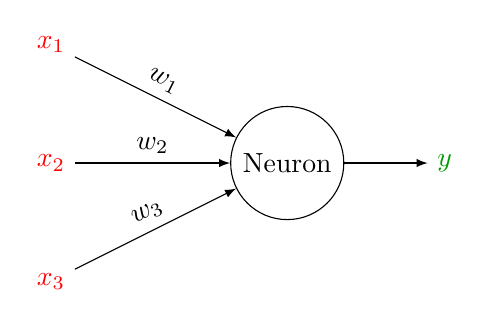
\begin{tikzpicture}[>=latex]
    \path (3,0) node [circle,draw](neuron){Neuron};
    \path[red] (0,1.5) node(x1){$x_1$} (0,0) node(x2){$x_2$} (0,-1.5) node(x3){$x_3$};
    \path[black!40!green] (5,0) node(y1){$y$};
    \draw[->] (x1) -- node[above,sloped]{$w_1$} (neuron);
    \draw[->] (x2) -- node[above,sloped]{$w_2$} (neuron);
    \draw[->] (x3) -- node[above,sloped]{$w_3$} (neuron);
    \draw[->] (neuron) -- (y1);
  \end{tikzpicture}
  \caption{Perzeptron mit drei Inputs}
  \label{fi:perzeptron}
\end{figure}
\para{}
Fuer das Trainieren des Perzeptrons existieren spezielle Verfahren, welche hier
aber nicht relevant sind. Das Gradientenverfahren kann naemlich nicht verwendet
werden. Der Grund dafuer sollte spaeter in Sektion (\ref{sec:kuenstlicheNeuronen}) einleuchtend werden.

\para{}
\cite{wiki:perzeptron}
\cite{Nielsen}

\subsection{Was kann ein Perzeptron erlernen?}
Nun stellt sich die Frage, was ein Perzeptron erlernen kann und wofuer es genutzt werden kann.
Das Perzeptron ist lediglich ein \keyword{linearer Klassifikator} der Form
$y = w_1x_1 + \cdots + w_m x_m$. Es ist also ein Klassifizierungsmodell, kein Regressionsmodell.
Es kann die Features in zwei Klassen 0 oder 1 einordnen, wobei der Output der
Hypothesenfunktion, diese Klassifizierung angibt.
Ueberschreitet $y$ den Schwellenwert, werden die Features der Klasse 1 zugeordnet, sonst
der Klasse 0.
Jedoch muessen diese Klassen linear separierbar sein.
\para{}
Lineare Separierbarkeit bedeutet, dass alle Featurevektoren $\vec{x}_1,\ldots,\vec{x}_p \in \set{R}^m$
innerhalb ihres Vektorraums $\set{R}^m$ durch eine Hyperebene in ihre Klassen aufteilbar sein muessen.
Falls das Perzeptron zwei Inputs hat, bedeutet dies, dass die Ortsvektoren
einfach durch eine Gerade voneinander trennenbar sein muessen (siehe Abb.
(\ref{fig:linearer_Klassifikator})). \\
Falls die Features nicht linear separierbar sind, bedeutet dies, dass das
Perzeptron die Klassifizierung nicht erlernen kann.
BEISPIEL
\\
\begin{figure}[h!]
  \caption{erfolgreiche lineare Separierung (links) und das Versagen bei XOR (rechts)}
  \label{fig:linearer_Klassifikator}
\end{figure}
\para{}
\cite{wiki:perzeptron}
\cite{wiki:linear_separability}

\section{Erweiterung der Kuenstlichen Neuronen}\label{sec:kuenstlicheNeuronen}
Ein Perzeptron ist, wie vorhin erklaert, nur in der Lage, lineare Klassifikationen
durchzufuehren. Um nun auch kompliziertere Probleme zu loesen, muss das Prinzip
ausgebaut werden. Ausserdem brauchen wir ein Kuenstliches Neuron, welches sich
besonders gut als Baustein fuer KNNs eignet.


\subsection{Kuenstliche Neuronen im Allgemeinen}
Kuenstliche Neuronen sind immer so aufgebaut, dass sie einen oder mehrere Inputs
haben und einen einzigen Output. Zu jedem Input $x_i$ ist ein Gewicht
$w_{i}$ assoziert. Zuerst wird die gewichtete Summe der Inputs $\tilde{z}$ gebildet.
Die Neigung $b$ wird ebenfalls draufaddiert, um $z$ zu erhalten. Nun muss
die sogenannte \keyword{Aktivierung} $a$ gebildet werden. Sie ist der Output des Neurons.
Die Aktivierung $a = \varphi(z)$ ist das Resultat der
\keyword{Aktivierungsfunktion} $\varphi: \set{R} \to \set{R}$ angewendet
auf $z$. Die verschiedenen Kuenstlichen Neuronen unterscheiden
sich fast nur in ihrer Aktivierungsfunktion.
\\
\begin{figure}[h!]

  \caption{ein kuenstliches Neuron und seine Bestandteile}
\end{figure}
\\

\para{}
\cite{Nielsen}
\cite{wiki:kuenstliches_neuron}

\subsection{Perzeptronen als Kuenstliche Neuronen}
Zuerst noch einmal ein Blick auf das Perzeptron im Angesicht der Aktivierungsfunktion.
Ein wesentlicher Unterschied des Perzeptron gegenueber sonstigen Kuenstlichen
Neuronen, besteht darin, dass seine Inputs und Outputs nur binaere Werte
annehmen koennen. Um dieses Verhalten des Perzeptrons zu erhalten,
muss eine Stufenfunktion als Aktivierungfunktion verwendet werden: die Heaviside-Funktion $\Theta$.
Sie hat einen einzigen Stufensprung bei $x=0$ vom Wert 0 auf 1 (siehe Abb. (\ref{fig:heaviside})).
\\
\begin{figure}[h!]
  \begin{minipage}[h!]{0.5\textwidth}
    \begin{equation*}
      \varphi^{\text{hlim}}(z) = \Theta(z) =
      \begin{cases}
        1 & \quad \text{falls } z \geq 0\\
        0 & \quad \text{falls } z < 0
      \end{cases}
    \end{equation*}
  \end{minipage}
  \begin{minipage}[h!]{0.5\textwidth}
    \centering
    \begin{tikzpicture}[scale=2.5]
      \draw[->] (-1.5,0) -- (1.5,0) node[right] {$x$}; % x-axes
      \draw[->] (0,-0.2) -- (0,1.2) node [above] {$y$}; % y-axes
      \draw[style=help lines,step=0.5] (-1.4,0) grid (1.4, 1.1);

      \foreach \x in {-1,-0.5,0.5,1}
      \draw[shift={(\x,0)}] (0pt,2pt) -- (0pt,-2pt) node[below,fill=pagecolor] {$\x$};

      \foreach \y in {0.5,1}
      \draw[shift={(0,\y)}] (2pt,0pt) -- (-2pt,0pt) node[left,fill=pagecolor] {$\y$};

      \draw[shift={(0,0)}] (0pt,0pt) node[below left,fill=pagecolor] {$O$};

      \draw[red,ultra thick] (-1.5,0) -- (0,0); % 0-red
      \draw[red,ultra thick] (0,1) -- (1.5,1); % 1-red
      \draw[red,ultra thick,dashed] (0,0) -- (0,1); % y-red
      \draw[draw=red,fill=white] (0,0) circle (0.05);
      \draw[draw=red,fill=red] (0,1) circle (0.05);
    \end{tikzpicture}
  \end{minipage}
  \caption{Definition und Graph der Heaviside-Funktion $\Theta$}
  \label{fig:heaviside}
\end{figure}

\cite{wiki:kuenstliches_neuron}
\cite{wiki:perzeptron}


\subsection{ReLU Neuronen}\label{sec:ReLU}
Der naechste Schritt nach einer Stufenfunktion als Aktivierungsfunktion, waren
lineare Aktivierungsfunktionen. Fuer diese koennen die Inputs nun belibige reelle
Zahlen sein.
Jedoch sind solche lineare Neuronen in einem KNN von keinem Nutzen.
Das hat den Grund, dass eine Verkettung von linearen Neuronen,
immer auf eine einzige lineare Funktion reduziert werden kann. Somit hat
die Verkettung keinen Mehrwert.
\para{}
Stattdessen verwendet man sogennante ReLU Neuornen. Sie benutzen die
\keyword{Rectified Linear Unit} (\keyword{ReLU}) Aktivierungsfunktion.
Diese ist
eine nur teilweise lineare Aktiverungsfunktion. Die Werte groesser als 0 werden
auf sich selber linear abbgebildet und die Werte kleiner als 0 werden auf 0
abbgebildet (siehe Abb. (\ref{fig:relu})).
Eine sehr wichtige Eigenschaft von ihr ist, dass sie - im Gegensatz zu den vorhin
genannten Aktivierungsfunktionen - fast ueberall differenzierbar%
\footnote{%
  Eigentlich ist die ReLU-Funktion in $x=0$ wegen des Knicks nicht
  differenzierbar. Fuer die Gradientenberechnung definiert man jedoch einfach
  die Ableitung $\varphi^{\text{ReLU}}'(0) \coloneqq 0$. Dies ist mathematisch zwar nicht
  korrekt, loest aber das Problem.
}%
und strikt monoton
steigend ist. Erst fuer diese Aktivierungsfunktion, kann das Gradientenverfahren
angewendet werden und somit das KNN trainiert werden.
\para{}
Da sie nur teilweise linear ist, gehoert sie genaugenommen den
Nicht-linearen-Aktiverungsfunktionen an. Diese Nicht-Linearitaet erlaubt es dem
Neuronen deutlich komplexere Systeme zu modellieren und so deutlich komplexere
Probleme zu loesen. Wir werden in Sektion (\ref{sec:UAT}) sogar erfahren, dass
eine Kompostion von nicht-linearen Neuroen jede beliebige Funktion approximieren kann.
\para{}
Wir werden diese Art von Neuron vorerst zur Seite legen und erst wieder in
Kapitel (\ref{sec:CNN}) im Zusammenhang mit KNNs zur Bilderkennung betrachten.
\para{}
\begin{figure}[h!]
  \begin{minipage}[h!]{0.5\textwidth}
    \begin{equation}
      \varphi^{\text{ReLU}}(z) =
      \begin{cases}
        z & \quad \text{falls } z > 0\\
        0 & \quad \text{falls } z \leq 0
      \end{cases}
      = \max(z,0)
    \end{equation}
  \end{minipage}
  \begin{minipage}[h!]{0.5\textwidth}
    \centering
    \begin{tikzpicture}[scale=2.5]
      \draw[->] (-1.5,0) -- (1.5,0) node[right] {$x$}; % x-axes
      \draw[->] (0,-0.2) -- (0,1.2) node [above] {$y$}; % y-axes
      \draw[style=help lines,step=0.5] (-1.4,0) grid (1.4, 1.1);

      \foreach \x in {-1,-0.5,0.5,1}
      \draw[shift={(\x,0)}] (0pt,2pt) -- (0pt,-2pt) node[below,fill=pagecolor] {$\x$};

      \foreach \y in {0.5,1}
      \draw[shift={(0,\y)}] (2pt,0pt) -- (-2pt,0pt) node[left,fill=pagecolor] {$\y$};

      \draw[shift={(0,0)}] (0pt,0pt) node[below left,fill=pagecolor] {$O$};

      \draw[red,ultra thick] (-1.5,0) -- (0,0);
      \draw[red,ultra thick] (0,0) -- (1,1);
      \draw[red,ultra thick,dashed] (1,1) -- (1.2,1.2);

      \draw[draw=red,fill=red] (0,0) circle (0.03);
    \end{tikzpicture}
  \end{minipage}
  \caption{Formel und Graph der ReLU-Funktion}
  \label{fig:relu}
\end{figure}

\para{}
\cite{wiki:kuenstliches_neuron}
\cite{Nielsen}

\subsection{Sigmoid Neuronen}
Ein weiteres nicht-lineares Neuron, sind sogennante Sigmoid-Neuronen.
Den Namen haben sie von ihrer Aktivierungsfunktion: der Sigmoidfunktion $\sigma$.
\para{}
Auch sie kann aufgrund ihrer Nicht-linearitaet zur Approximation jeder Funktion
in einem KNN verwendet werden. Sie ist die Aktivierungsfunktion, welche am
meisten in KNNs eigesetzt wird. Da sie wirklich sehr stark von Lineartiaet
abweicht und so am schnellsten komplexe Sachverhalte modellieren kann.
\para{}
Die Sigmoid-Funktion besitzt eine einzige Wendestelle $\sigma''(x=0)=0$ und hat
zwei Asymptoten, eine $\ds\lim_{x \to -\infty} \sigma(x)=0$
und eine zweite $\ds\lim_{x \to \infty} \sigma(x)=1$ (siehe Abb.
(\ref{fig:sigmoid})). Desweiteren zeichnet sie sich durch ihre simple Ableitung aus.
\\
\begin{figure}[h!]
  \begin{minipage}[h!]{0.5\textwidth}
    \begin{align*}
      \varphi^{\text{sig}}(z) &= \sigma(z) = \frac{1}{1 + e^{-z}}\\
      \sigma'(z)&=\sigma(z)(1-\sigma(z))
    \end{align*}
  \end{minipage}
  \begin{minipage}[h!]{0.5\textwidth}
    \centering
    \begin{tikzpicture}[scale=2.5]
      \draw[->] (-1.5,0) -- (1.5,0) node[right] {$x$}; % x-axes
      \draw[->] (0,-0.2) -- (0,1.2) node [above] {$y$}; % y-axes
      \draw[style=help lines,ystep=0.5,xstep=0.25] (-1.4,0) grid (1.4, 1.1);

      \foreach \x/\xtext in {-1/-4,-0.5/-2,0.5/2,1/4}
      \draw[shift={(\x,0)}] (0pt,2pt) -- (0pt,-2pt) node[below,fill=pagecolor] {$\xtext$};

      \foreach \y in {0.5,1}
      \draw[shift={(0,\y)}] (2pt,0pt) -- (-2pt,0pt) node[left,fill=pagecolor] {$\y$};

      \draw[shift={(0,0)}] (0pt,0pt) node[below left,fill=pagecolor] {$O$};

      \draw[red,ultra thick,x=0.25cm] plot[domain=-6.0:6.0] (\x,{1/(1+exp(-\x)) });
    \end{tikzpicture}
  \end{minipage}
  \caption{Definition, Ableitung und Graph der Sigmoid-Funktion $\sigma$}
  \label{fig:sigmoid}
\end{figure}

\para{}
\cite{wiki:kuenstliches_neuron}
\cite{wiki:sigmoidfunktion}


\section{Topologie der Kuenstlichen Neuronalen Netzen}
Nun sollten diese Sigmoiden Neuronen als Bausteine verwendet werden, um ein Kuenstliches
Neuronales Netz zu bilden. Dazu werden sie miteinander verbunden und bilden so ein Netz,
aehnlich wie ein Nervensystem.
\para{}
Diese Neuronen sind in verschieden Schichten (engl.: Layers)
arangiert. Die erste ist die \keyword{Inputschicht}. Sie beinhaltet die
Inputneuronen. Diese sind eigentlich keine richtigen
Neuronen sondern eher Platzhalter fuer ihr jeweiliges Feature $x_i$. Als letztes kommt die
\keyword{Outputschicht} mit den Outputneuronen, welche jeweils einen Outputwert $y_i$
besitzen. Dazwischen liegen die \keyword{Zwischenschichten} (engl.: hiddenlayers). Von ihnen kann es
beliebig viele geben und in ihnen beliebig viele Neuronen.
Falls viele Zwischenschichten verwendet werden, bezeichnet man das Netzwerk als
``deep''. Daher ruert auch der Name des Deep Learnings.
Der Aufbau eines KNN bezeichnet man als \keyword{Topologie} des Netzes. Die
Topologie umfasst viele Hyperparameter. Darunter sind zum Beispiel die Anzahl Zwischenschichten, wie auch
die Anzahl Neuronen pro Schicht.
\para{}
Jedes Neuron aus einer Schicht ist mit jedem Neuron aus der naechsten Schicht ueber
Verbindungen gekoppelt. Alle Verbindungen besitzten ein Gewicht analog zu den Inputs des
Perzeptrons. Die Aktivierung, also der Output, eines Neurons wandert entlang den jeweiligen
Verbindung zu allen Neuronen der naechsten Schicht und dient als deren Input.
Die soeben beschriebe Art von KNN nennt man \keyword{Feedforward-Netz}, da alle Werte
ausschliesslich nach vorne propagiert werden.
\para{}
In Abbildung (\ref{fig:nn_layers}) ist ein Beispiel eines Neuronalen Netzes
abgebildet. In diesem Fall besitzt es sowohl 4 Inputs, als auch 4 Outputs. Es hat
ausserdem 3 Zwischenschichten. Die erste und die dritte haben jeweils 3 Neuronen
und die zweite besitzt 4 Neuronen. \\

\begin{figure}[h!]
  \centering
  \begin{tikzpicture}[>=latex]

    \tikzstyle{netstyle} = [matrix of nodes,nodes={draw,circle,inner sep=0, minimum size=1cm},column sep=0.5cm,row sep=-9pt]
    \tikzstyle{cl} = [draw=none,fill=none]
    \tikzstyle{heading} = [clear,text width=15mm,text centered]
    \tikzstyle{inp} = [fill=red!70!pagecolor]
    \tikzstyle{hid} = [fill=blue!70!pagecolor]
    \tikzstyle{ou} = [fill=green!70!pagecolor]

    \matrix[netstyle] (mat)
    {
      |[inp]| $x_1$     & |[cl]| & |[cl]| & |[hid]|$h_1^2$ & |[cl]| & |[cl]| & |[ou]|$y_1$ \\
      |[cl]| & |[cl]| & |[hid]|$h_1^1$   & |[cl]| & |[hid]|$h_1^3$ & |[cl]| & |[cl]| \\
      |[inp]| $x_2$     & |[cl]| & |[cl]| & |[hid]|$h_2^2$ & |[cl]| & |[cl]| & |[ou]|$y_2$ \\
      |[cl]| & |[cl]| & |[hid]|$h_2^1$   & |[cl]| & |[hid]|$h_2^3$ & |[cl]| & |[cl]| \\
      |[inp]| $x_3$     & |[cl]| & |[cl]| & |[hid]|$h_3^2$ & |[cl]| & |[cl]| & |[ou]|$y_3$ \\
      |[cl]| & |[cl]| & |[hid]|$h_3^1$   & |[cl]| & |[hid]|$h_3^3$ & |[cl]| & |[cl]| \\
      |[inp]| $x_4$     & |[cl]| & |[cl]| & |[hid]|$h_4^2$ & |[cl]| & |[cl]| & |[ou]|$y_4$ \\
    };

    % titels
    \node [yshift=1cm] at (mat-1-1) {Inputschicht};
    \node [yshift=1cm] at (mat-1-4) {Zwischenschichten};
    \node [yshift=1cm] at (mat-1-7) {Outputschicht};

    % dots
    % \node [yshift=-1cm,scale=2] at (mat-7-1) {$\vdots$}; % for inputs
    % \node [yshift=-1cm,scale=2] at (mat-6-3) {$\vdots$};
    % \node [yshift=-1cm,scale=2] at (mat-7-4) {$\vdots$};
    % \node [yshift=-1cm,scale=2] at (mat-6-5) {$\vdots$};
    % \node [yshift=-1cm,scale=2] at (mat-7-7) {$\vdots$}; % for outputs

    % input -> hidden1
    \foreach \ai in {1,3,...,7} {
      \foreach \aii in {2,4,6}
      \draw[->] (mat-\ai-1) -- (mat-\aii-3);
    }

    % hidden1 -> hidden2
    \foreach \ai in {2,4,...,6} {
      \foreach \aii in {1,3,...,7}
      \draw[->] (mat-\ai-3) -- (mat-\aii-4);
    }

    % hidden2 -> hidden3
    \foreach \ai in {1,3,...,7} {
      \foreach \aii in {2,4,6}
      \draw[->] (mat-\ai-4) -- (mat-\aii-5);
    }

    % hidden3 -> output
    \foreach \ai in {2,4,...,6} {
      \foreach \aii in {1,3,...,7}
      \draw[->] (mat-\ai-5) -- (mat-\aii-7);
    }


  \end{tikzpicture}
  \caption{Schichten eines KNNs}
  \label{fig:nn_layers}
\end{figure}

\cite{wiki:kuenstliches_neuronales_netz}
\cite{Nielsen}

\section{Lernverhalten}
Die Hoffnung beim Trainieren von KNNs besteht darin, dass das Modell fuer jede
weiter Schicht eine hoeheres Abstraktionsniveau erreicht. Wuerde man zum
Beispiel ein Netzwerk zur Gesichtserkennung trainieren, koennte man sich den
Erkennungsprozess folgendermassen vorstellen: Die erste Zwischenschicht erkennt
Kanten und Konturen. Die zweite vereint diese Merkmale zu Ecken und primitiven
geometrischen Formen. Die dritte Schicht sollte dann schon komplexere
geometrische Formen erkennen, welche gewissen Gesichtmerkmalen, wie der Nase, aehneln. Die letzten Schichten soll dann alle diese
Merkmale zusammensetzen und so ein Gesicht erkennen.
WEITERFUEHREN

\section{Vorwaertspropagierung}
Jetzt, da der Aufbau eines KNNs erklaert wurde, sollte nun die mathematische Funktionsweise
des Modells erklaert werden. Hierfuer muessen einige Konventionen zur
Bezeichnung der Teile eines KNNs getroffen werden. Es sollten vorallem noch
Abbildungen (\ref{fig:nomenklatur1}) und (\ref{fig:nomenklatur2}) zum
Verstaentnis der Nomenklatur studiert werden.
\begin{itemize}
\item{$l$ ist der Index einer Schicht. Die Indexierung beginnt bei 0.}
\item{$L$ ist der letzte Schichtindex und somit auch die gesamte Anzahl an
    Schichten (ohne die Inputschicht).}
\item{$|l|$ ist die Anzahl Neuronen in der $l$-ten Schicht.
    \footnote{
      Diese Schreibweise hat nichts mit dem Betrag zu tun, sondern wird einfach
      gewaehlt, da sie sehr platzsparend ist.
    }
  }
\item{$n_j^l$ bezeichnet das $j$-te Neuron in der $l$-ten Schicht.}
\item{$z_j^l$ ist die gewichtete Summe der Inputs des $j$-ten Neuron in der $l$-ten Schicht.}
\item{$a_j^l$ ist die Aktivierung/Output des $j$-ten Neurons in der $l$-ten Schicht.}
\item{$b_j^l$ ist die Neigung fuer das $j$-te Neuron in der ($l+1$)-ten Schicht.
    \footnote{
      Diese Konvention wurde gewaehlt, damit die folgenden Gleichungen simpler sind.
    }
  }
\item{$w_{j,k}^l$ ist das Gewicht der Verbindung vom $k$-ten Neuron
    in der $l$-ten Schicht zum $j$-ten Neuron in der ($l+1$)-ten Schicht.
    \footnote{
      Man beachte die Reihenfolge!\\
      Diese Konvention scheint zwar auf den ersten Blick unintuitiv, macht jedoch
      Sinn fuer die Matrixindezierung.
      (\ref{sec:backpropagation}).
    }
  }
\item{$\varphi$ ist die gewaehlte Aktivierungsfunktion (diese ist immer eine
    nicht-lineare Aktivierungsfunktion)}
\end{itemize}

\begin{figure}[h!]
  \centering
  \begin{tikzpicture}[>=latex]
    \tikzstyle{netstyle} = [matrix of nodes,nodes={draw,circle,inner sep=0, minimum size=1.25cm},column sep=0.5cm,row sep=-9pt]
    \tikzstyle{cl} = [draw=none,fill=none]
    \tikzstyle{sy} = [cl,font=\LARGE]
    \tikzstyle{heading} = [clear,text width=15mm,text centered]
    \tikzstyle{inp} = [fill=red!70!pagecolor]
    \tikzstyle{hid} = [fill=blue!70!pagecolor]
    \tikzstyle{ou} = [fill=green!70!pagecolor]

    \matrix[netstyle] (mat)
    {
      |[inp]|$n_1^0$     & |[cl]| & |[cl]| & |[cl]| & |[cl]| & |[cl]| & |[ou]|$n_1^L$ \\
      |[cl]| & |[cl]| & |[hid]|$n_1^1$   & |[sy]| $\cdots$ & |[hid]|$n_1^{L-1}$ & |[cl]| & |[cl]| \\
      |[inp]|$n_2^0$     & |[cl]| & |[cl]| & |[cl]| & |[cl]| & |[cl]| & |[ou]|$n_2^L$ \\
      |[cl]| & |[cl]| & |[hid]|$n_2^1$   & |[sy]| $\cdots$ & |[hid]|$n_2^{L-1}$ & |[cl]| & |[cl]| \\
      |[inp]|$n_3^0$     & |[cl]| & |[sy]| $\vdots$ & |[cl]| & |[sy]| $\vdots$ & |[cl]| & |[ou]|$n_3^L$ \\
      |[sy]| $\vdots$ & |[cl]| & |[hid]|$n_{|1|}^1$ & |[sy]|$\cdots$ & |[hid]|$n_{|L-1|}^{L-1}$ & |[cl]| & |[sy]| $\vdots$ \\
      |[inp]|$n_{|0|}^0$ & |[cl]| & |[cl]| & |[cl]| & |[cl]| & |[cl]| & |[ou]|$n_{|L|}^L$ \\
    };

    % titels
    \node [yshift=1.5cm] at (mat-1-1) {Inputschicht};
    \node [yshift=1.5cm] at (mat-2-4) {Zwischenschichten};
    \node [yshift=1.5cm] at (mat-1-7) {Outputschicht};

    % input -> hidden1
    \foreach \ai in {1,3,...,7} {
      \foreach \aii in {2,4,...,6}
      \draw[->] (mat-\ai-1) -- node[above,sloped]{} (mat-\aii-3);
    }

    % hidden1 ->...
    \foreach \ai in {2,4,...,6} {
      \foreach \aii in {2,4,...,6} {
        \node (A) at (mat-\ai-3) {};
        \node (B) at (mat-\aii-5) {};
        \draw[left color=black,right color=white] (mat-\ai-3) -- ($(A)!0.3!(B)$);
      }
    }

    % ...-> hidden2
    \foreach \ai in {2,4,...,6} {
      \foreach \aii in {2,4,...,6} {
        \node (A) at (mat-\ai-3) {};
        \node (B) at (mat-\aii-5) {};
        \draw[left color=black,right color=white] ($(A)!0.7!(B)$) -- (mat-\aii-5);
      }
    }

    % hidden3 -> output
    \foreach \ai in {2,4,...,6} {
      \foreach \aii in {1,3,...,7}
      \draw[->] (mat-\ai-5) -- node[above,sloped]{} (mat-\aii-7);
    }

    \node[below=2mm of mat-7-1.south] {$l=0$};
    \node[below=2mm of mat-6-3.south] {$l=1$};
    \node[below=2mm of mat-6-5.south] {$l=L-1$};
    \node[below=2mm of mat-7-7.south] {$l=L$};
  \end{tikzpicture}
  \label{fig:nomenklatur1}
  \caption{zum Verstaentniss der Nomenklatur}
\end{figure}
\para{}
\begin{figure}[h!]
  \centering
  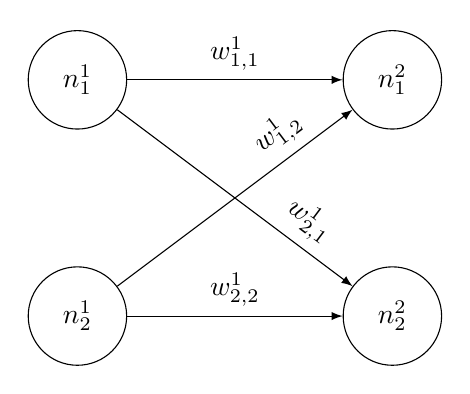
\begin{tikzpicture}[>=latex]
    \path (-2,1.5) node [draw,circle,inner sep=0,minimum size=1.25cm](n11){$n^1_1$};
    \path (-2,-1.5) node [draw,circle,inner sep=0,minimum size=1.25cm](n12){$n^1_2$};
    \path (2,1.5) node [draw,circle,inner sep=0,minimum size=1.25cm](n21){$n^2_1$};
    \path (2,-1.5) node [draw,circle,inner sep=0,minimum size=1.25cm](n22){$n^2_2$};
    \draw[->] (n11) -- node[above,sloped]{$w^1_{1,1}$} (n21);
    \draw[->] (n11) -- node[above,pos=0.75,sloped]{$w^1_{2,1}$} (n22);
    \draw[->] (n12) -- node[above,pos=0.75,sloped]{$w^1_{1,2}$} (n21);
    \draw[->] (n12) -- node[above,sloped]{$w^1_{2,2}$} (n22);
  \end{tikzpicture}
  \label{fig:nomenklatur2}
  \caption{zum Verstaentnis der Gewichtebeschriftungen}
\end{figure}
\para{}
Die Vorwaertspropagierung beginnt bei den Inputneuronen, welche jeweils
einen Inputwert in sich tragen. Diese Werte werden, um fuer eine kohaerente Nomenklatur zu sorgen,
analog zu den Aktivierungen der anderen Neuronen mit $a_j^0$ bezeichnet, wobei
$j$ der Index des Neurons ist. \\
Nun muessen die restlichen Aktivierungen der Neuronen bis und mit den Ouputneuronen berechnet werden. Dies geschieht rekursiv, anhand der
Aktivierungen der voherigen Schicht und zwar folgendermassen (ersichtlich in
Gleichung (\ref{eq:gewichtete_summe_normal})).
\para{}
Zuerst laeuft eine Summe ueber alle Neuronen $n_k^{l}$ der jetztigen Schicht
$l$. Dabei wird die gewichtete Summe der Aktivierungen $a_k^{l}$ mit den
assozierten Gewichten $w_{j,k}^l$ gebildet. ZU KOMPLIZIERT RELEVANT?: Hierbei ist das Gewicht jenes, welches das
$k$-te Neuron der $l$-ten Schicht mit dem $j$-ten Neuron der ($l+1$)-ten Schicht verbindet.
Zusaetzlich gehoert zu der gewichteten Summe auch die jeweilige Neigung $b_j^l$, welche
dazuaddiert wird. Diese gewichtete Summe wird mit $z_j^{l+1}$ bezeichnet.
\\
\begin{equation}\tag{FP1}\label{eq:gewichtete_summe_normal}
  z_j^{l+1} = \sum_{k=1}^{|l|} w_{j,k}^l a_k^l + b_j^l
\end{equation}
\\
Auf diese Summe wird dann die Aktivierungsfunktion $\varphi$ angewandt.
Das ist dann die Aktivierung $a_j^{l+1}$ des $j$-ten Neurons in der ($l+1$)-ten Schicht.
\\
\begin{equation}\tag{FP2}\label{eq:aktivierung_normal}
  a_j^{l+1} = \varphi\left(\sum_{k=1}^{|l|} w_{j,k}^l a_k^{l} + b_j^l \right) = \varphi \left( z_j^{l+1} \right)
\end{equation}
\par\bigskip
Fuer Deep Learning braucht man vorallem sogenannte Deep Neural Networks. Diese
zeichnen sich dadurch aus, dass sie sehr viele Zwischenschichten besitzen.
Deshalb bezeichnet man sie auch als ``deep''.
Bei solchen Netzwerken ist es nicht unueblich,
dass diese sehr viele Neuronen und Verbindungen (ueber 100'000) besitzen.
Um hierbei nicht den Ueberblick zu verlieren und um nicht in den Indizes zu
ertrinken, macht man Gebrauch von \keyword{Linearer Algebra}. Man verwendet
Matrizen und Vektoren um die vielen Variabeln zusammenzufassen.
Ausserdem besteht ein weiterer Vorteil darin, dass Computer mithilfe von Vektor-
und Matrixoperationen die Berechnungen paralellisieren koennen und in kuerzerer
Zeit und mit weniger Ressourcen viele Berechnungen gleichzeitig ausfuehren koennen.
Dies beschleunigt das Training der Modelle um
ein Vielfaches. Dies wird spaeter in Sektion
(\ref{sec:tensorflow}) noch weiter thematisiert.
\para{}
Die Inputs $\vec{x}$, Vorhersagen $\vec{y}$ und Labels $\vec{\hat{y}}$ haben wir schon von Anfang an als Vektoren geschrieben.
Nun sollen noch die Modellparameter und die restlichen Komponenten eines KNNs als Vektoren und Matrizen zusammengefasst werden.
Sowohl alle gewichteten Summen $z_j^l$, wie auch alle Aktivierungen $a_j^l$
einer Schicht $l$, werden in Vektoren $\vec{z}^l \in \set{R}^{|l|}$ und
$\vec{a}^l \in \set{R}^{|l|}$ zusammengefasst.
Auch alle Neigung $b_j^l$ fuer eine Schicht ($l+1$) bilden einen Vektor
$\vec{b}^l \in \set{R}^{|l+1|}$.
\para{}
Zu guter letzt, wird noch eine \keyword{Gewichtsmatrix} $\mat{W}^l \in
\set{R}^{|l+1| \times |l|}$
definiert. Sie enthaelt alle Gewichte welche die $l$-te
Schicht \textit{zu} der ($l+1$)-ten Schicht verbindet.
Das heisst der Eintrag in der $j$-ten Zeile und in
der $k$-ten Spalte ist $w_{j,k}^l$ und verbindet so das Neuron $n_k^{l}$ zu
dem Neuron $n_j^{l+1}$.
\\
\begin{align*}
  \vec{z}^l &=  \trans{\begin{pmatrix} z_1^l & z_2^l & \cdots & z_{|l|}^l \end{pmatrix}} \\
  \vec{a}^l &=  \trans{\begin{pmatrix} a_1^l & a_2^l & \cdots & a_{|l|}^l \end{pmatrix}} \\
  \vec{b}^l &=  \trans{\begin{pmatrix} b_1^l & b_2^l & \cdots & b_{|l+1|}^l \end{pmatrix}} \\
\end{align*}
\begin{equation*}
  \mat{W}^l =
  \begin{pmatrix}
    w_{1,1}^l & w_{1,2}^l & \cdots & w_{1,|l|}^l \\[0.3em]
    w_{2,1}^l & w_{2,2}^l & \cdots & w_{2,|l|}^l \\[0.3em]
    \vdots & \vdots & \ddots & \vdots \\[0.3em]
    w_{|l+1|,1}^l & w_{|l+1|,2}^l & \cdots & w_{|l+1|,|l|}^l
  \end{pmatrix}
\end{equation*}
\\
Mit diesen Definitionen kann nun fast Gleichung (\ref{eq:gewichtete_summe_normal}) in
Matrixform geschrieben werden, denn die Matrixmultiplikation von $\mat{W}^l$ mit
$\vec{a}^{l}$ ergibt einen Vektor $\vec{\tilde{z}}^{l+1}$, welcher alle gewichteten
Summen $\tilde{z}_j^{l+1}$ ohne die jeweilige Neigung enthaelt.
\\
\begin{equation*}
  \mat{W}^l \vec{a}^{l} = \trans{\begin{pmatrix}\ds \sum_{j=1}^{|l|} w_{1,j}^l a_j^l &\ds \sum_{j=1}^{|l|} w_{2,j}^l a_j^l & \cdots &\ds \sum_{j=1}^{|l|} w_{|l+1|,j} a_j^l \end{pmatrix}} = \vec{\tilde{z}}^{l+1}
\end{equation*}
\\
Nun muessen wir noch den Neigungsvektor $\vec{b}^l$ draufaddieren und wir
erhalten Gleichung (\ref{eq:gewichtete_summe_matrix}), mithilfe der wir den
Vektor der gewichteten Summen $\vec{z}^{l+1}$ bilden koennen.
\\
\begin{equation}\tag{FP1a}\label{eq:gewichtete_summe_matrix}
  \vec{z}^{l+1} = \mathbf{W}^{l} \vec{a}^{l} + \vec{b}^{l}
\end{equation}
\\
Der letzte Schritt besteht noch darin die Aktivierungsfunktion auf $\vec{z}^{l+1}$
anzuwenden um den Aktivierungsvektor $\vec{a}^{l+1}$ zu bilden.
Hierfuer muss aber noch ein neues mathematisches
Konzept eingefuehrt werden: die Vektorisierung einer Funktion.
\para{}

\begin{defbox}{Vektorisierung einer Funktion}
  Die Vektorisierung einer skalaren Funktion $f$, geschrieben als
  $\vecf{f}[\vec{v}]$ hat als Argument einen Vektor $\vec{v}$, auf dessen
  Komponenten jeweils \textit{einzeln} die Funktion $f$ angewandt wird. Dieser neue
  Vektor ist der Rueckgabewert der Funktion. Er besitzt die gleichen Dimensionen
  wie der Argumentvektor.
  \\
  \begin{equation*}
    \vecf{f}[\vec{v}]=
    \begin{pmatrix}
      f(v_1)\\
      \vdots \\
      f(v_n)\\
    \end{pmatrix}
  \end{equation*}
\end{defbox}

Nun kann ganz einfach die vektorisierte Aktivierungsfunktion $\vecf{\varphi}$ auf
$\vec{z}^{l+1}$ angewandt werden.

\begin{equation}\tag{FP2a}\label{eq:aktivierung_matrix}
  \vec{a}^{l+1} = \vecf{\varphi} \left[\mat{W}^{l} \vec{a}^{l} + \vec{b}^{l} \right] = \vecf{\varphi} \left[ \vec{z}^{l+1} \right]
\end{equation}

\para{}
\cite{Nielsen}

\subsection{Modellparameter initialisieren}\label{sec:parameter_initalisieren}
Ein Schritt der getan werden muss, bevor das Training beginnt, ist das
Initialisieren aller Modellparameter, in diesem Fall die Gewichte und Neigungen.
Dies ist ein sehr essentieller Schritt, denn diese Startwerte entscheiden
erheblich ueber die Leistungsfaehigkeit des Modells.
\para{}
Wie in Sektion (\ref{sec:gradientenverfahren}) gezeigt, muss am Anfang des
Gradientenverfahrens ein Startpunkt $\vec{p}_0$ innerhalb des Gradientenfeldes
$\vecf{\nabla}C$ gewaehlt werden, von welchem aus der Gradientenabstieg beginnt.
Da wir das Gradientenverfahren zur Optimierung der Modellparameter verwenden,
ist unser Startpunkt der Vektor aller Hyperparameter
$\vec{\param} = \trans{\begin{pmatrix} \param_1 & \cdots & \param_k \end{pmatrix}}$.
Dieser Startpunkt entscheidet darueber, in welches lokale Minimum konvergiert
wird und bestimmt somit auch die bestmoegliche Exaktheit der Vorhersagen. Falls
schlechte Initialwerte gewaehlt werden, konvergiert der Punkt in ein hohes lokales
Minimum, was grosse Kostenfunktionswerte und schlechte Vorhersagen verursacht.
\para{}
Es ist nicht moeglich im Vorhinein zu wissen, welche Initialwerte gute Resultate
liefern. Man muss ausprobieren, deshalb initialisert man gaengierweise die
Hyperparameter mit Zufallswerten. Dafuer nimmt man aber nicht irgendwelche
Zufallsvariabeln sondern man benutzt die Gauss'sche Normalverteilung
$\mathcal{N}(\mu,\sigma^2)$ bzw. ihre Dichtefunktion.
\[\ds \phi(x\ |\ \mu,\sigma^2) = \frac{1}{\sqrt{2\pi\sigma^2}} \text{exp} \left\{-\frac{{(x-\mu)}^2}{2\sigma^2}\right\} \]
\para{}

\ifcp
\pgfplotsset{compat=1.15}
\pgfmathdeclarefunction{gauss}{2}{%
  \pgfmathparse{1/(#2*sqrt(2*pi))*exp(-((x-#1)^2)/(2*#2^2))}%
}
\pgfmathdeclarefunction{gausseval}{3}{%
  \pgfmathparse{1/(#2*sqrt(2*pi))*exp(-((#3-#1)^2)/(2*#2^2))}%
}
\usetikzlibrary{arrows.meta}    % <--- added

\begin{figure}[h!]
  \centering
  \begin{tikzpicture}[
    every pin/.style = {pin edge={Latex-,thin,black}},>=latex
    ]
    \begin{axis}[
      width=15cm,height=6cm,
      scale only axis,
      axis lines=middle,
      ymin=0,ymax=0.45,
      axis line style = thick,
      xtick={-3,-2,-1,1,2,3},
      x label style={anchor=west},
      y label style={anchor=south},
      extra x ticks={0},
      extra x tick style={%
        grid=major,
        ticklabel pos=top,
      },
      extra x tick labels={$\mu$},
      xlabel={$x$},
      ylabel={$\phi(x)$},
      axis on top,
      samples=50]
      \addplot[pattern=north west lines,pattern color=blue!25,domain=-3.5:3.5] {gauss(0,1)} \closedcycle;
      \addplot[domain=-3.5:3.5,red,thick] {gauss(0,1)};
      \node[fill=red,circle,minimum size=0.15cm,inner sep=0] (wp1) at (-1,{gausseval(0,1,-1)}) {};
      \node[fill=red,circle,minimum size=0.15cm,inner sep=0] (wp2) at (1,{gausseval(0,1,1)}) {};
      \coordinate (zero) at (0,0);
      \newcommand{\equal}{=}
      % \path [fill=black] (wp1) circle (2pt);
      % \path [fill=black] (wp2) circle (2pt);
      \path [draw=black,<->,very thick] (wp1) -- node[above]{$\sigma^2$} (wp1 -| zero);
      \path [draw=black,<->,very thick] (wp2) -- node[above]{$\sigma^2$} (wp2 -| zero);
      \node [pin=120:$\phi(x_{WS1})'' \equal 0$] at (wp1) {};
      \node [pin=60:$\phi(x_{WS2})'' \equal 0$] at (wp2) {};

      \node [pin=60:$\ds A \equal \int_{-\infty}^{\infty} \phi(x) \text{d}x \equal 1$] at (1.4,0.05) {};
    \end{axis}
  \end{tikzpicture}
  \caption{Graph der Dichtefunktion $\phi(x\ |\ \mu=0,\sigma^2=1)$ mit ihren
    wichtigsten Eigenschaften}%
\end{figure}
\fi


Um die Neigungen $b_{t=0}$ zu initialisieren benutzt man eine Normalverteilung
$\mathcal{N}(0,1)$ mit Erwartungswert $\mu = 0$ und Varianz $\sigma^2 =
1$. Um die Gewichte $w_{t=0}$ zu initialisieren benutzt man ebenfalls eine
Normalverteilung mit Erwartungswert $\mu = 0$, jedoch wird die Varianz
$\sigma^2$ so skaliert, dass die Summe aller Zufallesvariabeln der Gewichte
einer Schicht eine Varianz von $\sigma^2_{tot} = 1$ hat. ERKLAEREN
\begin{align}
  w_{t=0}^l &\sim \mathcal{N}(\mu = 0, \sigma^2 = \frac{1}{|l|}) \\
  b_{t=0}^l &\sim \mathcal{N}(\mu = 0, \sigma^2 = 1)
\end{align}


\para{}
\cite{wiki:normal_distribution}
\cite{Nielsen}

\section{Rueckwaertspropagierung}\label{sec:backpropagation}
Die wahre Herausforderung besteht beim Gradientenverfahren darin,
die partiellen Ableitungen der Modellparameter,
also die Komponenten des Gradienten, zu bestimmen.
Anders gesagt muessen alle Terme
$\ds\partderiv{C}{w_{j,k}^l}$, wie auch alle Terme $\ds\partderiv{C}{b_k^l}$
berechnet werden.
Das Verfahren zum bestimmen dieser Ausdruecke ist so spezifisch und aufwendig,
dass das Gradientenverfahren fuer KNNs einen eigenen Namen hat: die
\keyword{Rueckwaertspropagierung} (engl.: backpropagation) (auch Fehlerrueckfuehrung).
Im Verlauf der Arbeit ist es nicht notwendig die Rueckwaertspropagierung bis ins
Detail zu verstehen. Man sollte lediglich ein Gespuer dafuer entwickeln, wie
der Gradient berechnet wird.
\para{}
Da ein KNN, wie der Name es schon sagt, vernetzt ist, koennen die partiellen
Ableitungen einer Schicht bezueglich seiner Nachbarsschichten berechnet werden.
Dies ist auch der namensgebende Grundgedanke der Rueckwaertsprogagierung: Man
beginnt in der letzten Schicht die partiellen Ableitungen zu bestimmen und
berechnet dann im Rueckwaertsgang Schicht fuer Schicht die vorherigen
partiellen Ableitungen, bis zur Inputsschicht. \\
Dies macht man mithilfe der Kettenregel der Ableitungen.
Es ist sinnvoll fuer das Aufstellen dieser Gleichungen das Netzwerk als
\keyword{Computation Graph} zu betrachten.
\para{}
Ein Computation Graph ist eine Darstellung einer Verkettung von Funktionen als Netzwerk von Operationen.
Die Knoten im Graph stellen Variabeln dar und die Pfade, welche die Knoten
verbinden, sind die Funktionen, welche die Variabeln aufeinander abbilden. Die
Funktion wird auf die Variable angewandet, von der der Pfad ausgeht. Der Knoten
in welchem der Pfad endet, nimmt dann den Funktionswert an. Falls
mehrere Pfade in einem Knoten enden, werden die einzelnen Werte der Pfade
zusammenaddiert, um die Variable zu bilden. KETTENREGEL NOCHMALS ERWAEHNEN ODER
IN ABBILDUNG (LEIBNIZ-SCHREIBWEISE!)\\
In Abbildung (\ref{fig:computation_graph}) ist ein Beispiel eines Computation
Graphs zusammen mit der Herleitung der partiellen Ableitungen dargestellt.
\para{}
\begin{figure}[h!]
  \begin{minipage}[h!]{0.5\textwidth}
    \centering
    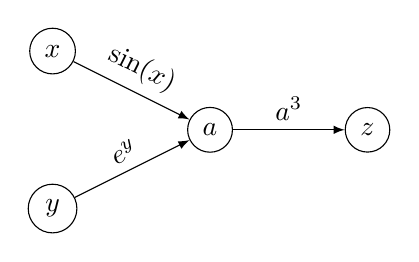
\begin{tikzpicture}[>=latex]

      \path (0,1) node [circle,draw](var_x){$x$};
      \path (0,-1) node [circle,draw](var_y){$y$};
      \path (2,0) node [circle,draw](var_a){$a$};
      \path (4,0) node [circle,draw](var_z){$z$};
      % \path[red] (0,1.5) node(x1){$x_1$} (0,0) node(x2){$x_2$} (0,-1.5) node(x3){$x_3$};
      \draw[->] (var_x) -- node[above,sloped]{$\sin(x)$} (var_a);
      \draw[->] (var_y) -- node[above,sloped]{$e^y$} (var_a);
      \draw[->] (var_a) -- node[above,sloped]{$a^3$} (var_z);

    \end{tikzpicture}

  \end{minipage}
  \begin{minipage}[h!]{0.5\textwidth}
    \begin{align*} % or align*
      a(x,y) &= \sin(x) + e^y \\
      z(a(x,y)) &= a^3(x,y) = \left(\sin(x) + e^y\right)^3 \\[3ex]
      \partderiv{z}{x} &= \partderiv{a}{x} \cdot  \partderiv{z}{a} = \cos(x) \cdot 3a^2 \\[0.5ex]
      \partderiv{z}{y} &= \partderiv{a}{y} \cdot \partderiv{z}{a} = e^y \cdot 3a^2
    \end{align*}
  \end{minipage}

  \caption{Computation Graph einer exemplarischen Verkettung von Funktionen}
  \label{fig:computation_graph}
\end{figure}
\para{}
Der erste Schritt der Rueckwaertsprogagierung besteht darin, dass man die partiellen Ableitungen $\ds\partderiv{C}{z_j^l}$
der Kostenfunktion $C$ bezueglich den gewichteten Summen $z_j^l$ aller Schichten
berechnet. Daraus laesst sich dann spaeter sehr einfach die partiellen Ableitungen
bezueglich den Gewichten $\ds\partderiv{C}{w_{j,k}^l}$ und bezueglich den Neigung
$\ds\partderiv{C}{b_j^l}$ berechnen.
\para{}
Zur Uebersichtlichkeit definiert man einen \keyword{Fehler} $\delta_j^L$ fuer
jedes $j$-te Neuron in jeder $l$-ten Schicht, welcher die partielle Ableitung bezueglich der
gewichteten Summe dieses Neurons ist (siehe Gl. (\ref{eq:BP0)}). Ebenfalls definiert man analog einen Fehlervektor
$\vec{\delta}^l$, welcher alle Fehler $\delta_j^l$ einer Schicht $l$
zusammenfasst (siehe Gl. (\ref{eq:BP0a})). Nun heisst es diesen fuer jedes Neuron jeder Schicht zu
berechnen.
\\
\begin{gather}
  \tag{BP0}\label{eq:BP0} \delta_j^l \coloneqq \partderiv{C}{z_j^l} \\
  \tag{BP0a}\label{eq:BP0a} \vec{\delta}^l \coloneqq \trans{\begin{pmatrix} \ds\partderiv{C}{z_1^l} & \ds\partderiv{C}{z_2^l} & \cdots & \ds\partderiv{C}{z_{|l|}^l} \end{pmatrix}}
\end{gather}
\\
Da die Kostenfunktion unmittelbar auf die letzte Schicht $L$ angewandt wird, beginnt
man auch dort mit der Berechnung des Fehlers $\vec{\delta}^L$.
Wir stellen nun einen Computation Graph auf, um die partiellen Ableitungen zu bilden.
\para{}
\begin{figure}[h!]
  \centering
  \begin{tikzpicture}[>=latex]
    % \colorlet{sumcolor}{red!70!textcolor}
    % \colorlet{actcolor}{green!70!textcolor}
    % \tikzstyle{act} = [fill=actcolor]
    % \tikzstyle{sum} = [fill=sumcolor]

    \path (0,2) node [circle,draw](z1){$z_1^L$};
    \path (0,0) node [circle,draw](z2){$z_2^L$};
    \path (0,-2) node [circle,draw](z3){$z_3^L$};
    \path (3,2) node [circle,draw](a1){$a_1^L$};
    \path (3,0) node [circle,draw](a2){$a_2^L$};
    \path (3,-2) node [circle,draw](a3){$a_3^L$};
    \path (6,0) node [circle,draw](C){$C$};

    \draw[->] (z1) -- node[above,sloped]{$\varphi(z_1^L)$} (a1);
    \draw[->] (z2) -- node[above,sloped]{$\varphi(z_2^L)$} (a2);
    \draw[->] (z3) -- node[above,sloped]{$\varphi(z_3^L)$} (a3);

    \draw[->] (a1) -- node[above,sloped]{$c(a_1^L,\hat{y}_1$)} (C);
    \draw[->] (a2) -- node[above,sloped,pos=0.4]{$c(a_2^L,\hat{y}_2$)} (C);
    \draw[->] (a3) -- node[above,sloped]{$c(a_3^L,\hat{y}_3$)} (C);

    % endings
    \node (beg1) at (-3,2) {};
    \node (beg2) at (-3,0) {};
    \node (beg3) at (-3,-2) {};

    \draw[dashed] ($(beg1)!0.6!(z1)$) -- (z1);
    \draw[dashed] ($(beg1)!0.6!(z2)$) -- (z2);
    \draw[dashed] ($(beg1)!0.6!(z3)$) -- (z3);
    \draw[dashed] ($(beg2)!0.6!(z1)$) -- (z1);
    \draw[dashed] ($(beg2)!0.6!(z2)$) -- (z2);
    \draw[dashed] ($(beg2)!0.6!(z3)$) -- (z3);
    \draw[dashed] ($(beg3)!0.6!(z1)$) -- (z1);
    \draw[dashed] ($(beg3)!0.6!(z2)$) -- (z2);
    \draw[dashed] ($(beg3)!0.6!(z3)$) -- (z3);
  \end{tikzpicture}
  \caption{Computation Graph zur Berechnung von $\vec{\delta}^L$}
  \label{fig:cg_L}
\end{figure}
\para{}
Wir koennen dem Computation Graph aus Abbildung (\ref{fig:cg_L}) entnehmen, dass die Kosten $C$ eine Funktion
in Abhaengigkeit von den letzten Aktivierungen $a_j^L$ ist, welche wiederum in
Abhaengigkeit von der jeweiligen gewichteten Summe $z_j^L$ berechnet werden.
Somit koennen wir mithilfe der Kettenregel die Beziehung (\ref{eq:BPh1}) aufstellen.
\\
\begin{equation}\label{eq:BPh1}
  \delta_j^L = \partderiv{C}{z_j^L} = \partderiv{C}{a_j^L} \cdot \partderiv{a_j^L}{z_j^L}
\end{equation}
\\
Da $a_j^L$ durch die Anwendung der Aktivierungsfunktion $\varphi$ auf $z_j^L$
gebildet wird, ist $\ds\partderiv{a_j^L}{z_j^L}$ einfach die Ableitung der Aktivierungsfunktion
$\varphi'(z_j^L)$. Somit erhalten wir die erste (\ref{eq:BP1}) von vier
wichtigen Gleichungen fuer die Rueckwaertsprogagierung.
\\
\begin{equation}\tag{BP1}\label{eq:BP1}
  \delta_j^L = \partderiv{C}{a_j^L} \cdot \varphi'(z_j^L)
\end{equation}
\\
Nun moechten wir diese Ausdruecke wieder in Matrixschreibweise realisieren,
welche die ganze Schicht $L$ zusammenfasst. Dazu
muss eine neue Operation eingefuehrt werden: das Hadamard-Produkt.

\begin{defbox}{Hadamard-Produkt}
  Das Hadamard-Produkt (auch elementweises Produkt) ist ein spezielles Produkt zweier gleichgrossen Matrizen
  $\mat{A} \in \set{R}^{m \times n}$ und $\mat{B} \in \set{R}^{m \times n}$.
  Die resultierende Matrix ergibt sich aus der elementweisen Multiplikation der Ausgangsmatrizen.

  \begin{minipage}{0.5\textwidth}
    \begin{equation*}
      \mat{A} \odot \mat{B} =
      \begin{pmatrix}
        \matelem{A}_{1,1} \matelem{B}_{1,1} & \cdots & \matelem{A}_{1,n} \matelem{B}_{1,n} \\[0.3em]
        \vdots & \ddots & \vdots \\[0.3em]
        \matelem{A}_{m,1} \matelem{B}_{m,1} & \cdots & \matelem{A}_{m,n} \matelem{B}_{m,n} \\[0.3em]
      \end{pmatrix}
      \in \set{R}^{m \times n}
    \end{equation*}
  \end{minipage}
  %
  \begin{minipage}{0.5\textwidth}
    \begin{equation*}
      \vec{v} \odot \vec{w} =
      \begin{pmatrix}
        v_1 w_1 \\
        \vdots \\
        v_n w_n
      \end{pmatrix}
    \end{equation*}

  \end{minipage}
\end{defbox}
\para{}

Mit $\vecf{\varphi}'$ als die vektorisierte Ableitung der Aktivierungsfunktion,
koenne wir den Fehlervektor der letzten Schicht nach Gleichung (\ref{eq:BPh0}) berechnen.

\begin{equation}\label{eq:BPh0}
  \vec{\delta}^L = \trans{\begin{pmatrix} \ds\partderiv{C}{a_1^L} & \ds\partderiv{C}{a_2^L} & \cdots & \ds\partderiv{C}{a_{|L|}^L}\end{pmatrix}} \odot \vecf{\varphi}'[\vec{z}^L]
\end{equation}

Dabei ist der erste Operand des Hadamard-Produkts nichts anderes als
der Gradient $\vecf{\nabla}_{\vec{a}^L} C$ der Kostenfunktion $C$ bezueglich dem Aktivierungsvektor
$\vec{a}^L$ der letzten Schicht. Dieser Gradient kann einfach berechnet werden, indem man die
vektorisierte Ableitungsfunktion fuer die gewaehlte Kostenfunktion bildet. Wuerde man die
Mittlere quadratischen Abweichung $C = \frac{1}{2|L|}(\vec{\hat{y}} - \vec{a}^L)^2$ als Kostenfunktion waehlen, haetten wir
$\vecf{\nabla}_{\vec{a}^L} C = (\vec{a}^L - \vec{\hat{y}}) \cdot \frac{1}{|L|}$.
\para{}
Daraus folgt die kompakte matrix-version (\ref{eq:BP1a}) der Gleichung
(\ref{eq:BP1}), welche den Fehlervektor fuer die letzte Schicht berechnet.
\\
\begin{equation}\tag{BP1a}\label{eq:BP1a}
  \vec{\delta}^L = \vecf{\nabla}_{\vec{a}^L}C \odot \vecf{\varphi}'(\vec{z}^L)
\end{equation}
\\
Nun muessen wir eine rekursive Berechnungsmethode des Fehlers $\delta_j^{l-1}$
der vorherigen Schicht anhand des Fehlers $\delta_j^l$ der jetzigen Schicht
erarbeiten. Dafuer stellen wir zuallererst wieder einen Computation Graph auf
(siehe Abb. (\ref{fig:cg_L-1})).
\para{}
\begin{figure}[h!]
  \centering
  \begin{tikzpicture}[>=latex]
    \path (0,1) node [circle,draw](z1-){$z_1^{l-1}$};
    \path (0,-1) node [circle,draw](z2-){$z_2^{l-1}$};
    \path (3,1) node [circle,draw](a1-){$a_1^{l-1}$};
    \path (3,-1) node [circle,draw](a2-){$a_2^{l-1}$};
    \path (7,2) node [circle,draw](z1){$z_1^l$};
    \path (7,0) node [circle,draw](z2){$z_2^l$};
    \path (7,-2) node [circle,draw](z3){$z_3^l$};

    \draw[->] (z1-) -- node[above,sloped]{$\varphi(z_1^L)$} (a1-);
    \draw[->] (z2-) -- node[above,sloped]{$\varphi(z_2^L)$} (a2-);

    \draw[->] (a1-) -- node[sloped,above]{$\times w_{1,1}$} (z1);
    \draw[->] (a1-) -- node[sloped,above,pos=0.8]{$\times w_{2,1}$} (z2);
    \draw[->] (a1-) -- node[sloped,below,pos=0.65]{$\times w_{3,1}$} (z3);
    \draw[->] (a2-) -- node[sloped,above,pos=0.65]{$\times w_{1,2}$} (z1);
    \draw[->] (a2-) -- node[sloped,above,pos=0.65]{$\times w_{2,2}$} (z2);
    \draw[->] (a2-) -- node[sloped,below]{$\times w_{3,2}$} (z3);

    % endings
    \node (beg1) at (-3,1) {};
    \node (beg2) at (-3,-1) {};
    \draw[dashed] ($(beg1)!0.6!(z1-)$) -- (z1-);
    \draw[dashed] ($(beg1)!0.6!(z2-)$) -- (z2-);
    \draw[dashed] ($(beg2)!0.6!(z1-)$) -- (z1-);
    \draw[dashed] ($(beg2)!0.6!(z2-)$) -- (z2-);

    \draw[dashed] (z1) -- ++(1.5,0);
    \draw[dashed] (z2) -- ++(1.5,0);
    \draw[dashed] (z3) -- ++(1.5,0);

  \end{tikzpicture}
  \caption{Computation Graph zur Berechnung von $\delta_j^{l-1}$}
  \label{fig:cg_L-1}
\end{figure}
\para{}
Es gilt erneut die Gleichung (\ref{eq:BPh1}) fuer die Berechnung des Fehlers $\delta_j^{l-1}$.
\\
\begin{equation}\tag{\ref{eq:BPh1}}
  \delta_j^{l-1} = \partderiv{C}{z_j^{l-1}} = \partderiv{a_j^{l-1}}{z_j^{l-1}} \cdot \partderiv{C}{a_j^{l-1}}
\end{equation}
\\
Zuerst einmal ist der erste Faktor wieder die Ableitung $\varphi'(z_j^{l-1})$ der Aktiverungsfunktion.
Desweiteren beeinflusst beim Uebergang der Schicht ($l-1$) zur Schicht $l$ eine Aktivierungen
$a_j^{l-1}$ alle gewichteten Summen $z_k^l$. Mit der Kettenregel folgt daher,
dass die partielle Ableitung $\ds\partderiv{C}{a_j^{l-1}}$ die Summe aller
$\ds\partderiv{C}{z_k^l} \cdot \ds\partderiv{z_k^l}{a_j^{l-1}}$ sein muss. Wir
erhalten Gleichung (\ref{eq:BPh2}).
\\
\begin{equation}\label{eq:BPh2}
  \delta_j^{l-1} = \varphi'(z_j^{l-1}) \cdot \sum_{k=1}^{|l|} \left( \partderiv{C}{z_k^l} \cdot \partderiv{z_k^l}{a_j^{l-1}} \right)
\end{equation}
\\
Um die gewichtete Summe $z_k^l$ zu bilden, multipliziert man einfach die
Aktivierung $a_j^{l-1}$ der vorherigen Schicht mit den entsprechenden Gewichten $w_{k,j}^{l-1}$.
Dadurch ist diese partielle Ableitung $\ds\partderiv{z_k^l}{a_j^{l-1}}$ gerade das
Gewicht selbst. Desweiteren ist $\ds\partderiv{C}{z_k^l}$ per Definition der
Fehler $\delta_k^l$. Mit dieser Erkenntnis erhalten wir die zweite essentielle
Gleichung (\ref{eq:BP2}) fuer die Rueckwaertsprogagierung.
\\
\begin{equation}\tag{BP2}\label{eq:BP2}
  \delta_j^{l-1} = \varphi'(z_j^{l-1}) \cdot \sum_{k=1}^{|l|} \left( \delta_k^l \cdot w_{k,j}^{l-1} \right)
\end{equation}
\\
Auch diese Gleichung haetten wir gerne in der Matrixschreibweise. Wir beginnen
mit der Erweiterung auf alle gewichteten Summen.
\\
\begin{equation*}
  \vec{\delta}^{l-1} = \vecf{\varphi}'[\vec{z}^{l-1}] \odot \trans{\begin{pmatrix} \ds\sum_{k=1}^{|l|} w_{k,1}^{l-1} \cdot \delta_k^l & \cdots & \ds\sum_{k=1}^{|l|} w_{k,|l-1|}^{l-1} \cdot \delta_k^l \end{pmatrix}}
\end{equation*}
\\
Der zweite Operant des Hadamard-Produkts ist hierbei gerade das Produkt der
Matrixmultiplikation zwischen
der transponierten Gewichtsmatrix $\trans{(\mat{W}^{l-1})}$ der Schicht ($l-1$)
und dem Fehlervektor $\vec{\delta}^l$ der Schicht $l$ (ersichtlich in folgender Gleichung).

\begin{gather*}
  \trans{\begin{pmatrix} \ds\sum_{k=1}^{|l|} w_{k,1}^{l-1} \cdot \delta_k^l & \cdots & \ds\sum_{k=1}^{|l|} w_{k,|l-1|} \cdot \delta_k^l \end{pmatrix}} =
  \begin{pmatrix}
    w_{1,1}^{l-1} & w_{2,1}^{l-1} & \cdots & w_{|l|,1}^{l-1} \\
    w_{1,2}^{l-1} & w_{2,2}^{l-1} & \cdots & w_{|l|,2}^{l-1} \\
    \vdots & \vdots & \ddots & \vdots \\
    w_{1,|l-1|}^{l-1} & w_{2,|l-1|}^{l-1} & \cdots & w_{|l|,|l-1|}^{l-1}
  \end{pmatrix}
  \trans{\begin{pmatrix} \delta_1^l & \cdots & \delta_{|l|}^l \end{pmatrix}} \\=
  \trans{\begin{pmatrix}
      w_{1,1}^{l-1} & w_{1,2}^{l-1} & \cdots & w_{1,|l-1|}^{l-1} \\
      w_{2,1}^{l-1} & w_{2,2}^{l-1} & \cdots & w_{2,|l-1|}^{l-1} \\
      \vdots & \vdots & \ddots & \vdots \\
      w_{|l|,1}^{l-1} & w_{|l|,2}^{l-1} & \cdots & w_{|l|,|l-1|}^{l-1}
    \end{pmatrix}}
  \vec{\delta}^l = \trans{(\mat{W}^{l-1})} \vec{\delta}^l
\end{gather*}

Nun haben wir unsere rekursive Fehlerdefinition in Matrixschreibweise und somit
die kompakte Version (\ref{eq:BP2a}) der zweiten wichtigen Formel (\ref{eq:BP2}).
\\
\begin{equation}\tag{BP2a}\label{eq:BP2a}
  \vec{\delta}^{l-1} = (\trans{(\mat{W}^{l-1})} \vec{\delta}^l) \odot \vecf{\varphi}'[\vec{z}^{l-1}]
\end{equation}
\\
In einem letzten Schritt muessen wir jetzt noch Formeln herleiten, mit welchen
man anhand des Fehlers $\delta_j^l$ die partiellen Ableitungen der Gewichte und
der Neigungen berechnen kann.
\para{}
Eine Neigung $b_j^l$ ist Funktionsbestandteil der entsprechenden gewichteten
Summe $z_j^{l+1}$. Somit gilt fuer die Neigung Formel (\ref{eq:BPh3}).
\\
\begin{equation}\label{eq:BPh3}
  \partderiv{C}{b_j^l} = \partderiv{C}{z_j^{l+1}} \cdot \partderiv{z_j^{l+1}}{b_k^l}
\end{equation}
\\
Der erste Term ist hierbei per Definition unser Fehler $\delta_j^{l+1}$ und der
zweite Term laesst sich zu 1 evaluieren, da die Summe $z_k^{l+1}$ nur aus
$b_k^l$ besteht und aus Summanden, welche fuer die partielle Ableitung als konstant gelten.
Somit ist die Ableitung der Neigung gerade unser Fehler und wir erhalten die
dritte (\ref{eq:BP3}) von vier essentielen Gleichungen.
\\
\begin{equation}\tag{BP3}\label{eq:BP3}
  \partderiv{C}{b_j^l} = \delta_j^{l+1}
\end{equation}
\\
Somit ist der Kostengradient bezueglich der Neigung gerade der Fehlervektor
(siehe Gl. (\ref{eq:BP3a})).
\\
\begin{equation}\tag{BP3a}\label{eq:BP3a}
  \vecf{\nabla}_{\vec{b^l}} C =  \vec{\delta}^{l+1}
\end{equation}
\\
Ein Gewicht $w_{j,k}^l$ ist ebenfalls ein Funktionsbestandteil der assozierten
gewichteten Summe $z_j^{l+1}$. Dadurch gilt fuer die partiellen Ableitungen der
Kosten nach dem Gewicht Gleichung (\ref{eq:BPh4}).
\\
\begin{equation}\label{eq:BPh4}
  \partderiv{C}{w_{j,k}^l} = \partderiv{C}{z_j^{l+1}} \cdot \partderiv{z_j^{l+1}}{w_{j,k}^l}
\end{equation}
\\
Dabei laesst sich der erste Teil wieder zum Fehler $\delta_j^{l+1}$ evaluieren.
Die zweite partielle Ableitung ist gerade die Aktivierung $a_k^l$, da sich die
gewichtete Summe aus der Multiplikation des Gewichtes mit der Aktivierung ergibt.
Somit erhalten wir die letzte der vier essentiellen Gleichungen (\ref{eq:BP4}).
\begin{equation}\tag{BP4}\label{eq:BP4}
  \partderiv{C}{w_{j,k}^l} = \delta_j^{l+1} \cdot a_k^l
\end{equation}
\\
Die Matrix-version davon ist Gleichung (\ref{eq:BP4a}).
\begin{equation}\tag{BP4a}\label{eq:BP4a}
  \vecf{\nabla}_{\mat{W}^l} C = \vec{\delta}^{l+1} \trans{(\vec{a^l})}
\end{equation}

ALLES ZUSAMMENFASSEN

\cite{Nielsen}


\section{Universal Approximation Theorem?}\label{sec:UAT}
Es stellt sich nun die Frage, was ein Neuronales Netz alles erlernen kann.
Diese Frage kann man mit dem \keyword{Universal Approximation Theorem} (UAT)
beantworten. Dieser Satz ist ein mathematischer Beweis dafuer, dass ein KNN
grundsaetzlich in der LAge ist jede kontinuerliche Funktion beliebig gut zu
approximieren. Er wurde von Kurt Hornik in 1991 beweisen.

Etwas genauer besagt der UAT, dass ein Feed-Forward Netzwerk mit einer einzigen
Zwischenschicht, welche eine endliche Anzahl Neuron hat, jede Kontinuierliche
Funktion approximieren kann. Voraussetzung dafuer ist, dass es sich bei den
Neuronen und Nicht-lineare-Neuronen handelt. Dies ist nur eine theoretische
Ausage ueber das Lernpotenzial eines KNNs. Jedoch macht es keinerlei Aussage
darueber, ob ein KNN wirklich die Funtkionen erlernen wird.

IAN GOODFELLOW:
A feedworward network with a single layer is sufficient to represent any
function, but the layer may be infeasibly large and may fail to lean and
generalize correctly.

Die meisten Klassen von Probleme koennen einfach als eine Funktion formuliert
werden. Somit bedeutet der UAT, dass ein KNN theoretisch jedes Problem loesen kann.

Der eigentliche Beweis ist mathematisch ziemlich anspruchsvoll, deshalb werden
wir diesen nicht behandeln.

AUF ANDERE RESOURCE (QR-CODE) VERWEISEN FUER ILLUSTRIEVEN BEWEIS ODER ANHANG VON
MIR GESCHRIEBEN

\cite{wiki:uat}


\pagebreak
\chapter{Convolutional Neural Networks}
Viele Anwendungen von Machine Learning sind verbunden mit Bild- oder
Audioverarbeitung, wie z.B Bildklassifizierung, Gesichtserkennung oder
Spracherkennung.
Vorallem aber fuer hochaufloesende Bilder sind die KNNs, die wir soeben
kennengelernt haben, nicht geeignet. Sie sind zum Teil gar nicht in der
Lage eine Korrelation zwischen den Inputs und Outputs zu erlernen.
Um diesen Umstand zu erklaeren, wird nun ein kleines Beispielmodell erlauetert:
\para{}
\label{sec:CNN_parameter_problem}
Es soll ein KNN designed werden, welches eine Photographie klassifizieren
soll, ob darauf ein Hund sichtbar ist oder nicht. Wir nehmen fuer dieses
Gedankenexperiment bereits ein relativ niedrig aufgeloestes Bild mit $256 \times 256$
Pixel, dies entspricht weniger als $0.07$ Megapixel (ein iPhone XS hat eine Kamera mit
12 Megapixel). Um die verschiedenen Farben zu codieren besitzt jeder Pixel drei Komponten: R, G
und B. Somit hat dieses Bild insgesamt $256 \times 256 \times 3 = 196'608$
Komponenten. Jede Komponente ist ein Feature welches das KNN zu verrechnen hat. Somit bestuende
die erste Schicht des Netzwerkes aus fast $200'000$ Neuronen. Um diese Schicht
nun mit seiner Nachbarsschicht, welche gleiche Dimensionen besitzt, zu verbinden, braucht
es $196'608 \times 196'608 = 38'654'705'664$ Verbindungen und damit gleich so
viele Gewichte! Fuer ein Netwerk ohne eine einzige Zwischenschichten gaebe es
also ueber 38 Milliarden Modellparameter zu erlernen! Dass dies nicht realistisch ist,
sollte auf der Hand liegen.
\para{}
Nicht nur die Anzahl Modellparameter sind ein Problem fuer KNNs in der
Bildverarbeitung, sondern es bestehen noch weiter Probleme.
Trotzdem sollte nun klar sein, dass eine andere Modellarchitektur noetig ist, um Machine
Learning auf Bilder anzuwenden. Fuer genau solche Anwendungen wurde eine modifizierte
Version eines KNNs entwickelt: das \keyword{Convolutional Neural Network} (CNN).
Im Allgemeinen sind CNNs immer dann geeignet, wenn es Daten zu verarbeiten gibt, welche eine
rasterartige Form haben, wie eben z.B Bilder.
Diese Art von Netzwerk macht Gebrauch von Konzepten aus der klassischen
Bildverarbeitung, wie sie mit beispielsweise Photoshop gemacht werden kann.
Wie beim Perzeptron und bei den klassischen KNNs auch, ist die Architektur
biologisch inspiriert.
Der folgende Abschnitt wird die Funktionsweise eines solchen CNNs erklaeren.
\para{}
\cite{Goodfellow-et-al-2016}
\cite{deeplearning.ai:cnn}
\cite{wiki:cnn}


\section{Bilder als Tensoren}\label{sec:tensor}
CNNs operieren an Bildern. Diese Bilder stellen den Input fuer die Modelle dar.
Um mit diesen Bildern rechnen zu koennen, ist es sinnvoll, sie als sogenannte
\keyword{Tensoren} vom Rang 3 zu untersuchen, anstatt sie als Anordnungen von
Pixeln zu betrachten. \\
Um zu verstehen, was ein Tensor dritten Ranges ist, muessen wir zuerst verstehen, was ein Tensor im Allgemeinen ist.

\begin{defbox}{Tensor}
  Ein Tensor $\ten{T}$ ist eine Verallgemeinerung von Skalaren, Vektoren und Matrizen auf
  $n$ Dimensionen. Es handelt sich wie bei Matrizen um
  eine Zahlenanordnung. Dabei wird die Anzahl Dimensionen, innerhalb welchen die
  Zahlen liegen als Rang oder Stufe $n$ des Tensors bezeichnet. Vorstellen kann man sich einen Tensor
  als ein Hyperrechteck mit $n$ Dimensionen, innerhalb dessen die Zahlen in
  einem Raster angeordnet sind. Diese Zahlen sind die Elemente des Tensors.
  Ein Tensor nullten Ranges ist ein Skalar, einer erster Stufe ein Vektor und
  einer mit Rang 2 ist eine normale Matrix.
  \begin{gather*}
    1 \in \set{R} \text{ (Skalar)} \quad \begin{pmatrix} 1 \\ 2 \\ 3 \end{pmatrix}
    \in \set{R}^3 \text{ (Vektor)} \quad
    \begin{pmatrix}
      1 & 2 & 3 \\
      4 & 5 & 6 \\
    \end{pmatrix} \in \set{R}^{2 \times 3} \text{ (Matrix)}
  \end{gather*}
\end{defbox}

\begin{defbox}{Tensor 3. Ranges}
  Ein Tensor $\ten{T} \in \set{R}^{h \times w \times d}$ mit Rang 3 ist eine 3-dimensionale Zahlenanordnung. Man kann sich
  diesen Tensor einfach als eine 3D-Matrix vorstellen; ein Volumen innerhalb
  dessen Zahlen in einem Raster angeordet sind.
  Analog zum Volumen bezeichnet man die Form des Tensors mit Hoehe, Breite und
  Tiefe. \\
  Ein Tensor von der Form $\set{R}^{3 \times 3 \times 3}$ koennte folgendermassen
  aussehen:
  \para{}



  % \begin{tikzpicture}[x=(15:.5cm), y=(90:.5cm), z=(330:.5cm), >=stealth]
  %   \draw (0, 0, 0) -- (0, 0, 10) (4, 0, 0) -- (4, 0, 10);
  %   \foreach \z in {0, 5, 10} \foreach \x in {0,...,3}
  %   \foreach \y [evaluate={\b=random(0, 1);}] in {0,...,3}
  %   \filldraw [fill=white] (\x, \y, \z) -- (\x+1, \y, \z) -- (\x+1, \y+1, \z) --
  %   (\x, \y+1, \z) -- cycle (\x+.5, \y+.5, \z) node [yslant=tan(15)] {\b};
  %   \draw [dashed] (0, 4, 0) -- (0, 4, 10) (4, 4, 0) -- (4, 4, 10);
  %   \draw [->] (0, 4.5, 0)  -- (4, 4.5, 0)   node [near end, above left] {Column};
  %   \draw [->] (-.5, 4, 0)  -- (-.5, 0, 0)   node [midway, left] {Row};
  %   \draw [->] (4, 4.5, 10) -- (4, 4.5, 2.5) node [near end, above right] {Channel};
  % \end{tikzpicture}

\end{defbox}
\newcommand{\arrayfilling}[2]{
  \fill[#2!30, opacity=.5] ([shift={(1mm,1mm)}]#1.north west) coordinate(#1auxnw)--([shift={(1mm,1mm)}]#1.north east)coordinate(#1auxne) to[out=-75, in=75] ([shift={(1mm,-1mm)}]#1.south east)coordinate(#1auxse)--([shift={(1mm,-1mm)}]#1.south west)coordinate(#1auxsw) to[out=105, in=-105] cycle;
  \fill[#2!80!black, opacity=1] (#1auxne) to[out=-75, in=75] (#1auxse) to[out=78, in=-78] cycle;
  \fill[#2!80!black, opacity=1] (#1auxnw) to[out=-105, in=105] (#1auxsw) to[out=102, in=-102] cycle;
}

\begin{tikzpicture}[font=\ttfamily,
  mymatrix/.style={
    matrix of math nodes, inner sep=0pt, color=#1,
    column sep=-\pgflinewidth, row sep=-\pgflinewidth, anchor=south west,
    nodes={anchor=center, minimum width=5mm,
      minimum height=3mm, outer sep=0pt, inner sep=0pt,
      text width=5mm, align=right,
      draw=none, font=\small},
  }
  ]

  \matrix (C) [mymatrix=green] at (6mm,5mm)
  {0 & 1 & 0 \\ -1 & 0 & 0\\ 0 & 0 & 0\\};
  \arrayfilling{C}{green}

  \matrix (B) [mymatrix=red] at (3mm,2.5mm)
  {0 & 0 & -1 \\ 0 & 0 & 0\\ 1 & 0 & 0\\};
  \arrayfilling{B}{red}

  \matrix (A) [mymatrix=purple] at (0,0)
  {0 & 0 & 0 \\ 0 & 0 & 1\\ 0 & -1 & 0\\};
  \arrayfilling{A}{purple}

  \foreach \i in {auxnw, auxne, auxse, auxsw}
  \draw[brown, ultra thin] (A\i)--(C\i);

  \node[left=1mm of B.west] {$\ten{T} =$};
  \node[right=3mm of B.east] {$\in \set{R}^{3 \times 2 \times 3}$};
\end{tikzpicture}
\para{}
Ein Bild kann somit einfach als Tensor dritten Ranges $\ten{B} \in \set{R}^{h
  \times w \times c}$, der Form $(\text{Bildhoehe} \times \text{Bildbreite}
\times \text{Anzahl Farbkomponenten})$ betrachtet werden.
Elemente der Matrix nehmen dann einfach die Werte der Pixelkomponenten an.
Ein schwarzweiss Bild hat nur eine Komponente, welche die Helligkeit angibt.
Somit waere es eine normale 2D-Matrix $\mat{B} \in \set{R}^{h \times w}$ (siehe
Abb. (\ref{fig:bildmatrix})).
\para{}
\begin{figure}[h!]
  \begin{tikzpicture}

  \end{tikzpicture}
  \caption{Beispiel einer Bildmatrix}
  \label{fig:bildmatrix}
\end{figure}

\cite{deeplearning.ai:cnn}
\cite{wiki:tensor}

\section{Topologie von CNNs}
Ein CNN besteht, wie auch ein KNN, aus Schichten. Jede dieser Schichten erhaelt
als Input ein Bild und hat auch wieder eines als Output. \\
Ein wichtiger Unterschied eines CNNs ist, dass es aus unterschiedlichen Typen von
Schichten besteht. Man unterscheiden zwischen vier Arten von Schichten:
\begin{itemize}
\item{\keyword{Fully-connected-Schichten},}
\item{\keyword{Convolutional-Schichten},}
\item{\keyword{Pooling-Schichten}, und}
\item{\keyword{Upsampling-Schichten}.}
\end{itemize}
Die Fully-Connected-Schicht ist altbekannt und ist einfach die klassische Schicht
eines KNNs, bestehend aus Neuronen. Aus diese werden wir nicht weiter eingehen,
da wir sie schon im vorherigen Kapitel kennengelernt haben. \\
Die Convolutional-Schicht ist eine neuartige Schicht, welche es im KNN nicht
gibt. Sie ist die Schicht, welche fuer das Training relevant ist,
da sie die Modellparameter beinhaltet. Sie extrahiert die relevanten Features
aus den Inputbildern und lernt so die Bilder zu verstehen. \\
Die Pooling-Schicht, wie auch die Upsampling-Schicht, beinhaltet keine
Modellparameter und sind deshalb fuer das Training nicht direkt relevant.
Diese Schichten werden lediglich gebraucht, um die verarbeiteten Bilder neu zu
skalieren. Dies ist sinnvoll, da durch die Extraktion gewisser Features, die
restlichen Features wegfallen. Somit muss weniger Information pro Bild gehalten
werden und die Bilder sollten schrumpfen, um Overfitting vorzubeugen. Die Pooling-
Schichten reduzieren die Bilder und die Upsampling-Schichten erweitern die
Bilder um mehr Pixel. Dies wird in Sektion (\ref{sec:autoencoder}) fuer die Autoencoder
hilfreich werden. \\
Grundsaetzlich folgt auf eine Convolutional-Schicht immer entweder eine Pooling-
oder eine Upsampling-Schicht. Somit bilden sie gewissermassen eine Einheit.
\para{}
In Abbildung (\ref{fig:cnn_topology}) ist ein Schema eines CNNs abbgebildet.
\begin{figure}[h!]

  \caption{Schichtung eines CNNs}
  \label{fig:cnn_topology}
\end{figure}

\para{}
\cite{Goodfellow-et-al-2016}
\cite{deeplearning.ai:cnn}
\cite{wiki:cnn}


\section{Convolutional-Schichten und Filter}
Zuerst betrachten wir die Convolutional Schicht. Diese Schicht macht ausgiebig
Gebrauch von sogenannten Filtern. Diese werden in diesem Abschnitt behandelt.

\subsection{Filter in der Bildverarbeitung}
\keyword{Filter} (auch Kerne) sind in der Bildverarbeitung sehr verbreitet. Jeder kennt sie entweder
von Photoshop, von Instagram oder sonstigen Bildbearbeitungsprogrammen.
Auch CNNs machen Gebrauch von solchen Filtern, in diesem Fall um die Features eines Bildes zu
erlernen.
\begin{figure}[h!]

  \caption{der Instagramfilter: Blablabla}
\end{figure}

\para{}
Ein Filter ist einfach eine Region, deutlich kleiner als das verarbeitete Bild
$\ten{B}$, welche
ueber alle Pixel wandert, diese manipuliert und so wieder ein neues Bild
$\tilde{\ten{B}}$ liefert.
Mathematisch gesehen handelt es sich bei einem Filter einfach um einen Tensor,
den sogennanten \keyword{Filtertensor} $\ten{F}$ oder Faltungstensor (siehe Abb.
(\ref{fig:filtermatrix})). Solche Filter sind immer quadratisch, wobei ihre
Zeilen- und Spaltenlaenge mit $f$ bezeichnet wird. Dabei ist $f$ immer eine ungerade Zahl, damit ein
Element, der sogennante \keyword{Zentralelement} (engl.: Center element), bezeichnet mit $(\ten{F})_C$,
immer im Zentrum des Filters liegt. \\

\begin{figure}[h!]
  % Sourcepixel kennzeichnen
  \caption{eine 2D-Filtermatrix}
  \label{fig:filtermatrix}
\end{figure}
\para{}
Das Verhalten des Filters wird durch seine Matrixeintraege bestimmt.
Die Elemente koennen also so gewaehlt werden, dass wenn der Filter auf ein Bild
angewandt wird, er bestimmte Features aus dem Bild hervorhebt. Solche Features
koennten zum Beispiel Raender oder Kanten sein, welche betont werden.
\para{}
Ein gutes Beispiel ist der Sobel-Filter. Er ist ein typischer 2D-Kantendetektions-Filter mit einer
Groesse von $f = 3$. Wir betrachten nun den Sobelfilter $\mat{G}_x$, welcher
horizontale Kanten akzentuiert. Die Eintraege dieses Filters lauten wie folgt:
\begin{equation*}
  \mat{G}_x =
  \begin{pmatrix}
    -1 & 0 & +1 \\
    -2 & 0 & +2 \\
    -1 & 0 & +1 \\
  \end{pmatrix}
\end{equation*}

Angewandt auf ein schwarz-weisses Bild, erhaelt man ein neues Bild, bei welchem alle erkannten
Kanten weiss eingefaerbt sind und die restlichen Bereiche schwarz sind.
Der Filter erkennt dabei jede Stelle als Kante, welche zwei Regionen mit
genug grossem Kontrast voneinander trennt.
In Abbildung (\ref{fig:sobel_filter}) wurde der horizontale Sobelfilter auf ein
Beispielbild angewandt. Links ist das Ursprungsbild und rechts ist das
prozessierte Bild.


\begin{figure}[h!]

  \caption{Sobel-Filter angewandt auf Beispielsbild}
  \label{fig:sobel_filter}
\end{figure}

\para{}
\cite{wiki:sobel_operator}
\cite{deeplearning.ai:cnn}
\cite{wiki:kernel}


\subsection{Filter in CNNs}
Aus didaktischen Gruenden betrachten wir nun zuerst
nur 2D-Filter, welche sich fuer graustufige Bilder
$\mat{B} \in \set{R}^{h \times w}$ eignen. Somit ist der hierfuer geeignete
Filter einfach eine 2D-Matrix, bezeichnet mit $\mat{F} \in \set{R}^{f \times
  f}$. Man bedenke bei jeder Filtermatrix einfach immer, dass es sich
eigentlich im allgemeinen Fall um einen 3D-Tensor handelt.
\para{}
Wie wir vorhin erfahren haben, koennen Filter genutzt werden um gewisse
Features eines Bildes hervorzuheben und andere Features zu ignorieren. Dabei
bestimmen die Filtereintraege, welche Features extrahiert werden. Somit besteht
die Aufgabe darin, die richtigen Filtereintraege zu bestimmen, damit die
gewuenschten Features erkannt werden und auf die gewuenschten Outputs abgebildet
werden. Naheliegend sollte jetzt der Gedanke sein, die Filtereintreage als die
Modellparameter eines CNNs zu definieren.
Mithilfe des Gradietenverfahrens sollten erneut diese Parameter
erlernt werden. \\
Da die Filter die gleiche Funktion haben, wie die Gewichte in einem KNN,
bezeichnet man die Filter in einem CNN mit $\mat{W}$. Die Groesse des Filters
stellt dabei einen Hyperparameter dar.

\begin{equation*}
  \mat{W} = \begin{pmatrix}
    w_{1,1} & \cdots & w_{1,f} \\
    \vdots & \ddots & \vdots \\
    w_{f,1} & \cdots & w_{f,f}
  \end{pmatrix}
\end{equation*}


\subsection{Filteroperation intutitiv}\label{sec:filteroperation_intuitiv}
Wie wendet man nun einen solchen Filter auf ein Bild an? Um das Prozedere einer
Filteroperation leichter verstaendlich zu machen, wird es erneut fuer ein
graustufiges Bild $\mat{B} \in \set{R}^{h \times w}$ erlauetert. Spaeter werden auch noch farbige
Bilder erklaert.
\para{}
Bei einer Filteroperation, wendet man einen Filter $\ten{W}$ auf einen Bildtensor
$\ten{B}$ an und erhaelt so ein neues Bild $\tilde{\ten{B}}$. Man schreibt dafuer:
$\tilde{\ten{B}} = \ten{W} * \ten{B}$.
\para{}
Um nun diese Operation zu erklaeren, verwenden wir als Beispiel eine
2D-Filtermatrix $\mat{W} \in \set{R}^{3 \times 3}$, bei welcher
$f = 3$ gewaehlt wurde.
Wie bereits oben erwaehnt, wandert der Filter ueber das Bild. Dabei befindet
sich der Filter immer ueber einer Region des Bilder, welche gleich gross ist,
wie der Filter selber (in diesem Fall ($3 \times 3$)), sodass den Filtermatrixeintraegen immer eindeutig
Bildmatrixeintraege entsprechen. Diese Region des Bildes bezeichnet man als das
\keyword{rezeptives Feld} des Filters (siehe Abb. (\ref{fig:receptive_field})).
Das Rezeptive Feld, bezeichnet mit $\hat{\mat{B}} \in \set{R}^{3 \times 3}$ ist also einfach eine
Untermatrix der Obermatrix $\mat{B}$.
\para{}
Jedem Element des Filters entspricht ein Element des rezeptiven Feldes. Dem
Zentralelement $(\mat{W})_c$ entspricht dabei gerade dem sogenannten Quellenpixel
(engl.: source pixel) $(\ten{B})_s$ des Bildes. Ihn verwenden wir fuer eine
Namenskonvention fuer das rezeptive Feld. Wir bezeichnen das rezeptive Feld mit
$\hat{\mat{B}}^{(y,x)}$, wobei die hochgestellten Indizes $(y,x)$ die Position
des Quellenpixel $(\mat{B})_S$ im Bild $\mat{B}$ angibt.

\begin{figure}[h!]

  % Zentralelement einzeichnen mit Beschriftung
  \caption{ein Filter und sein rezeptives Feld}
  \label{fig:receptive_field}
\end{figure}

\para{}
Der Filter beginnt nun oben links ueber das Bild zu wandern. Somit
hat der Filter zu beginn das rezeptive Feld $\hat{\mat{B}}^{(2,2)}$, denn der
Filter darf nicht ueber die Raender des Bildes hinausragen.
Nun werden die Elemente der Filters mit den Elementen des rezeptiven Feldes
verrechnet, welche die gleichen Dimensionen besitzen. Dabei wird einfach das
Hadamard-Produkt (das elementweise Produkt) des beiden Matrizen miteinander
gebildet. Nun erhalten wir eine neue Matrix $\mat{W} \odot
\hat{\mat{B}}^{(2,2)} = \mat{P} \in \set{R}^{3 \times 3}$.
Nun werden noch alle Elemente der neuen Matrix $\mat{P}$
aufsummiert. Diese Zahl ist dann der Grauwert des ersten Pixels $(\tilde{\mat{B}})_{1,1}$ des bearbeiteten
Bildes (siehe Gl. (\ref{eq:filter1})). In diesem Sinne stellt der Filter eine Gewichtung der Nachbarspixel dar, welche
bestimmt, wie die neuen Pixel aussehen.
\\
\begin{equation}\label{eq:filter1}
  (\tilde{\mat{B}})_{1,1} = \sum_{y=1}^3 \sum_{x=1}^3 (\mat{P})_{y,x}
\end{equation}
\\
Nun wird der Filter um ein Element nach rechts verschoben und die gleiche
Prozedur angewandt, um den zweiten Pixel zu berechnen. Dies
wird durchgezogen, bis eine ganze Zeile der Bildmatrix durchstreift wurde.
Danach wird der Filter wieder nach ganz links verschoben und er bewegt sich ein
Element nach unten. Das geschieht, bis das ganze Bild verrechnet wurde.
Dabei werden die Elemente des urspruenglichen Bildes durchaus mehrmals
verrechnet, da es zu einer Ueberlappung des vorherigen Filters und des
verschobenen Filters kommt.
\para{}

\ifcp
\begin{figure}[h!]
  \centering
  % 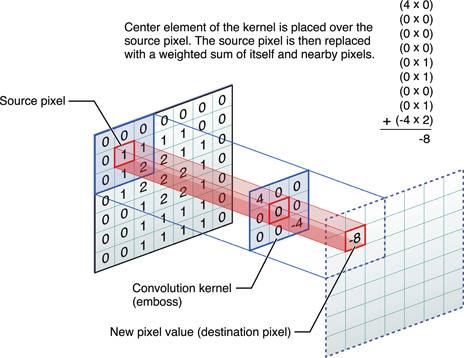
\includegraphics[width=0.5\textwidth]{conv.jpg}

  \makeatletter
  \tikzoption{canvas is xy plane at z}[]{%
    \def\tikz@plane@origin{\pgfpointxyz{0}{0}{#1}}%
    \def\tikz@plane@x{\pgfpointxyz{1}{0}{#1}}%
    \def\tikz@plane@y{\pgfpointxyz{0}{1}{#1}}%
    \tikz@canvas@is@plane
  }
  \makeatother

  \begin{tikzpicture}[x={(0.866cm,0.5cm)}, y={(-0.866cm,0.5cm)}, z={(0cm,1cm)}, scale=0.7,every pin/.style = {pin edge={Latex-,thin,black}}]


    \begin{scope}[canvas is xz plane at y=0,transform shape]
      % \draw[blue] (0,0) -- (10,0)--(10,10)--(0,10)--cycle;
      \foreach \ii [count = \xi] in {-3,-2,...,3}{
        \foreach \jj  [count = \yi] in {-3,-2,...,3}{
          \pgfmathsetmacro{\num}{int(abs(\ii)+abs(\jj))}
          \node[draw=blue!20!pagecolor,fill=blue!2!pagecolor,text=textcolor,minimum size=1cm] (n-1-\xi-\yi) at (\xi,-\yi) {\LARGE \num};
        }
      }
      \foreach \ii [count = \xi] in {-3,-2,-1}{
        \foreach \jj [count = \yi] in {-3,-2,-1}{
          \pgfmathsetmacro{\num}{int(abs(min(\ii,\jj))}
          \node[draw=blue!20!pagecolor,fill=blue!10!pagecolor,minimum size=1cm] (n-1-\xi-\yi) at (\xi,-\yi) {\LARGE \num}; % rename nodes
        }
      }

      \path[draw=textcolor] (n-1-1-1.north west) -- (n-1-7-1.north east) -- (n-1-7-7.south east) -- (n-1-1-7.south west) -- cycle;
      \path[draw=blue] (n-1-1-1.north west) -- (n-1-3-1.north east) -- (n-1-3-3.south east) -- (n-1-1-3.south west) -- cycle;


    \end{scope}

    \begin{scope}[canvas is xz plane at y=-7.3,transform shape]
      \foreach \ii [count = \xi] in {-1,0,1}{
        \foreach \jj  [count = \yi]in {-1,0,1}{
          \pgfmathsetmacro{\num}{int(\ii)}
          \node[draw=blue!20!pagecolor,fill=blue!10!pagecolor,text=textcolor,minimum size=1cm] (n-2-\xi-\yi) at (\xi,-\yi) {\LARGE \num};
        }
      }

      \path[draw=blue] (n-2-1-1.north west) -- (n-2-3-1.north east) -- (n-2-3-3.south east) -- (n-2-1-3.south west) -- cycle;
    \end{scope}

    \begin{scope}[canvas is xz plane at y=-11.2,transform shape]
      \foreach \ii [count = \xi] in {1,2,3,...,7}{
        \foreach \jj  [count = \yi]in {1,2,3,...,7}{
          \node[draw=blue!20!pagecolor,fill=blue!2!pagecolor,text=textcolor,minimum size=1cm] (n-3-\xi-\yi) at (\xi,-\yi) {};
        }
      }

      \foreach \ii [count = \xi] in {-3,-2,-1}{
        \foreach \jj [count = \yi] in {-3,-2,-1}{
          \pgfmathsetmacro{\num}{int(abs(min(\ii,\jj))}
          \node[draw=blue!20!pagecolor,fill=blue!10!pagecolor,minimum size=1cm] (n-3-\xi-\yi) at (\xi,-\yi) {}; % rename nodes
        }
      }

      \path[draw=blue,dashed] (n-3-1-1.north west) -- (n-3-3-1.north east) -- (n-3-3-3.south east) -- (n-3-1-3.south west) -- cycle;
      \path[draw=textcolor] (n-3-2-2.north west) -- (n-3-6-2.north east) -- (n-3-6-6.south east) -- (n-3-2-6.south west) -- cycle;
    \end{scope}

    % red box
    \path[draw=red,fill=red!50,opacity=0.3] (n-1-2-2.north east) -- (n-2-2-2.north east) -- (n-3-2-2.north east) -- (n-3-2-2.north west) -- (n-2-2-2.north west) -- (n-1-2-2.north west); % top
    \path[draw=red,fill=red!50,opacity=0.3] (n-1-2-2.south east) -- (n-2-2-2.south east) -- (n-3-2-2.south east) -- (n-3-2-2.south west) -- (n-2-2-2.south west) -- (n-1-2-2.south west); % bottom
    \path[draw=red,fill=red!50,opacity=0.3] (n-1-2-2.north east) -- (n-2-2-2.north east) -- (n-3-2-2.north east) -- (n-3-2-2.south east) -- (n-2-2-2.south east) -- (n-1-2-2.south east); % right
    \path[draw=red,fill=red!50,opacity=0.3] (n-1-2-2.north west) -- (n-2-2-2.north west) -- (n-3-2-2.north west) -- (n-3-2-2.south west) -- (n-2-2-2.south west) -- (n-1-2-2.south west); % left


    % blue lines connecting
    \path[draw=blue!40!pagecolor] (n-1-1-3.south west) -- (n-2-1-3.south west) -- (n-3-1-3.south west);
    \path[draw=blue!40!pagecolor] (n-1-3-1.north east) -- (n-2-3-1.north east) -- (n-3-3-1.north east);

    \node [pin=120:Rezeptives Feld $\hat{\mat{B}}^{(2,2)}$] at (n1-1-1.north west) {};
    \node [pin=180:Quellenpixel $(\mat{B})_S$] at (n1-2-2.east) {};
    \begin{scope}[canvas is xz plane at y=0,transform shape]
      \node[draw=red,minimum size=1cm] (marked1) at (2,-2) {\LARGE 2};
      % \node[] (sp-tag) at (n-1-2-2.north) {Quellenpixel $(\mat{B})_S$};
    \end{scope}

    \node [pin=180:Filter $\mat{F}$] at (n2-1-3.east) {};
    \begin{scope}[canvas is xz plane at y=-7.3,transform shape]
      \node[draw=red,text=textcolor,minimum size=1cm] (marked2) at (2,-2) {\LARGE 0};
      \node[] (rf-tag) at (n-2-2-1.north) {Filter $\mat{F}$};
      \node[] (ze-tag) at (n-2-2-2.north) {Zentralelement $(\mat{F})_C$};
    \end{scope}

    \begin{scope}[canvas is xz plane at y=-11.2,transform shape]
      \node[draw=red,fill=blue!10!white,text=textcolor,minimum size=1cm] (marked3) at (2,-2) {\LARGE -3};
    \end{scope}

  \end{tikzpicture}

  \caption{Schema, wie ein Filter ueber ein Bild laueft}
\end{figure}
\fi

Es ist zu bemerken, dass das neue Bild $\tilde{\mat{B}} \in \set{R}^{(h-2) \times (w-2)}$ nicht mehr die gleichen Masse
hat, wie das Ursprungsbild $\mat{B} \in \set{R}^{h \times w}$. Das liegt daran, dass pro
Lage des Filters jeweils nur ein Pixel des neuen Bildes berechnet wird. Man kann
sich vorstellen, dass an der Position des Quellenpixel jeweils ein neuer
Pixel entsteht. Dabei muss der Filter immer eine vollstaendige Region als
rezeptives Feld haben. Dadurch kommt das Zentralelement nie auf die Raender des
Bildes zu liegen. Somit fallen diese weg.
\para{}
\cite{deeplearning.ai:cnn}
\cite{wiki:convolution}

\subsection{Filteroperationen als diskrete Faltungen}
Eigentlich handelt es sich bei einer Anwendung eines Filters auf ein Bild um
eine spezifische mathematische Operation: eine \keyword{diskrete Faltung} (engl.:
\keyword{convolution}).
\footnote{
  Streng genommen wird in CNNs nicht eine diskrete Faltung durchgefuehrt, sondern
  eine sogenannte \keyword{Kreuzkorrelation}. Der Unterschied dabei ist, dass bei einer
  Kreuzkorrelation die Faltungsmatrix nicht zuerst horizontal, wie auch vertikal
  gespiegelt wird, im Gegensatz zu der eigentlichen Faltung. Jedoch verwendet man
  begrifflich das Wort Faltung fuer beide Operationen. Im Verlauf dieser Arbeit
  wird mit dem Wort Faltung immer die Kreuzkorrelation gemeint sein.
}
Daher ruehrt auch der Name des Convolutional Neural Networks.
Wir werden die Faltung als mathematische Operation nicht im vollen Umfang
betrachten, da sie relativ kompliziert ist. Wir werden uns lediglich auf die
Bedeutung der Faltung fuer Filter beschraenken.
\para{}
\begin{defbox}{Diskrete Faltung}
  Definintion Faltung
  \begin{equation}
    (f * g)(x) = \int_{-\infty}^{\infty} f(\tau) g(x-\tau) \text{d}\tau
  \end{equation}
\end{defbox}
\para{}
Mithilfe der Faltungsoperation koennen wir die Schritte welche in Sektion
(\ref{sec:filteroperation_intuitiv}) erklaert wurden zusammenfassen.
Bei der Filteroperation handelt es sich lediglich um eine diskrete Faltung des
Filtertensors $\ten{W}$ ueber den Bildtensor $\ten{B}$. Somit koennen wir
folgende Formel verwenden, um einen Pixel $\tilde{\mat{B}}(x,y)$ des neuen Bildes zu berechnen.
\\
\begin{equation}
  (\tilde{\mat{B}})_{y,x} = (\mat{W} * \mat{B})_{y,x} = \sum_{v=1}^{f} \sum_{u=1}^{f} (\mat{W})_{v,u}(\mat{B})_{y+v-1,x+u-1}
\end{equation}
\para{}
\begin{examplebox}{Faltung Beispielrechnung}
  \begin{equation*}
    \mat{B} =
    \begin{pmatrix}
      10 & 10 & 10 & 0 & 0 & 0 \\
      10 & 10 & 10 & 0 & 0 & 0 \\
      10 & 10 & 10 & 0 & 0 & 0 \\
      10 & 10 & 10 & 0 & 0 & 0 \\
      10 & 10 & 10 & 0 & 0 & 0 \\
      10 & 10 & 10 & 0 & 0 & 0 \\
    \end{pmatrix}
    \text{ und } \mat{W} =
    \begin{pmatrix}
      1 & 0 & -1 \\
      1 & 0 & -1 \\
      1 & 0 & -1 \\
    \end{pmatrix}
  \end{equation*}

  Fuer die Berechnung des ersten Pixels $(\tilde{\mat{B}})_{1,1}$ fuehren wir
  folgende Rechnung aus.
  \begin{align*}
    (\tilde{\mat{B}})_{1,1} &= (\mat{W} * \mat{B})_{1,1} = \sum_{v=1}^{f} \sum_{u=1}^{f} (\mat{W})_{u,v} (\mat{B})_{u,v} \\
    &= 10 \cdot 1 + 10 \cdot 0 + 10 \cdot -1 + 10 \cdot 1 + 10 \cdot 0 + 10 \cdot -1 + 10 \cdot 1 + 10 \cdot 0 + 10 \cdot -1 \\
    &= 0
  \end{align*}

  Das Gesamtergebniss lautet dann:
  \begin{equation*}
    \tilde{\mat{B}} = \mat{W} * \mat{B} =
    \begin{pmatrix}
      0 & 30 & 30 & 0 \\
      0 & 30 & 30 & 0 \\
      0 & 30 & 30 & 0 \\
      0 & 30 & 30 & 0 \\
    \end{pmatrix}
  \end{equation*}
\end{examplebox}
\para{}
Fuer farbige Bilder ist das Vorgehen praktisch das Selbe. Es werden nun
lediglich 3D-Tensoren anstatt 2D-Tensoren verwendet. Wir betrachten den
allgemeinen Bildtensor $\ten{B}_{h \times w \times c}$, wobei $c$ die Anzahl
Farbkomponenten (engl.: channels) ist.
Nun benutzt man einen Filter $\ten{W}_{f \times f \times c}$ mit beliebiger Groesse
$f$ aber mit der gleicher Tiefe $c$ wie das Ursprungsbild $\ten{B}$.
Dadurch muss der Filter nicht entlang der Tiefe des Bildes wandern, da er
gerade gleich tief ist wie das Bild. Das hat zur Folge, dass das verarbeitete
Bild $\tilde{\mat{B}}$ immer eine 2D-Matrix ist.
Die allgemeine Filtergleichung lautet:
\\
\begin{equation}\tag{FO}
  (\tilde{\mat{B}})_{y,x} = (\ten{W} * \ten{B})_{y,x} = \sum_{v=1}^{f} \sum_{u=1}^{f} \sum_{w=1}^c (\ten{W})_{v,u,w} (\ten{B})_{x+u-1,y+v-1,w}
\end{equation}

\para{}
\cite{Goodfellow-et-al-2016}
\cite{deeplearning.ai:cnn}
\cite{wiki:cnn}

\subsection{Mehrere Filter}
Eine Filteroperation ist nicht auf einen einzigen Filter beschraenkt. Es koennen
mehrere Filter auf das gleiche Ausgangsbild angewandt werden und zusammen ein
Endbild erzeugen.
\para{}
Die Anzahl Filter bezeichnen wir mit $c$.
Nun macht man pro Filter $\ten{W}_i$ eine Faltung ueber das Ursprungsbild $\ten{W}$, wobei
jede Faltung einen neue Matrix $\tilde{\mat{B}}_i = \ten{W}_i * \ten{B}$ liefert, wobei $i$ der Index des
Filters ist. All diese gefalteten Bilder $\tilde{\mat{B}}_i$ sind zweidimensionale Matrizen, unabhaengig davon, wieviele
Komponenten das Ursprungsbild hatte. Aus diesem Grund koennen die einzelnen
Matrizen $\tilde{\mat{B}}_i$ aufeinander gelegt werden und somit einen grossen 3D-Endtensor
$\tilde{\ten{B}}$ bilden.
Hierfuer muessen alle Filter $\ten{W}_i$ gleich gross sein.
\begin{figure}[h!]
  \caption{aufeinander gelegte gefaltene Bilder}

\end{figure}
Die Tiefe des neuen Bildes $\tilde{\ten{B}}$ ist jetzt gerade die Anzahl Filter $c$.
Wir haben bereits frueher immer die Tiefe des Bildes (bzw. die Anzahl
Farbkomponenten) mit $c$ bezeichnet. Somit ist $c$ sowohl die Anzahl Filter
einer Schicht, wie auch die Tiefe des verarbeiteten Bildes.

\para{}
\cite{Goodfellow-et-al-2016}
\cite{deeplearning.ai:cnn}

\subsection{Padding}
Wie bereits erwaehnt schrumpfen die Bilder (an den Raendern), wenn man einen Filter auf sie anwendet.
Zur Erinnerung: Dies liegt daran, dass pro Lage des Zentralelements nur ein Pixel
des neuen Bildes entsteht und das Zentralelement nunmal nicht auf allen
Ursprungspixeln zu liegen kommt. Die Raender fallen so weg. Diese Groesse des
Wegfalls haengt von der Filtergroesse $f$ ab. Hierbei gilt folgende Formel fuer die
neue Groesse $n_1$ des Bildes, anhand der alten Groesse $n_0$. $n$ bezeichnet
eine der zwei Seitenlaengen.
\begin{equation}
  n_1 = n_0 - f + 1
\end{equation}

Das Problem hierbei ist, dass nach einigen Faltungen das Bild extrem geschrumpft
ist und im Grenzfall kleiner als der Filter wird. Das darf natuerlich nicht
passieren. Ausserdem kommt es dabei zu einem relativen Informationverlust an den Raender, da es im
Innern des Bildes zu viel Ueberlappungen der Filterlagen kommt und es bei den
Raendern nur seltener zur Ueberlappung kommt.
\para{}
Diese Probleme werden mit sogenanntem \keyword{Padding} behoben. Padding ist ein
Schritt, welcher vor der eigentlichen Faltung stattfindet. Dabei werden einfach
zusaetzliche Raender (Zeilen und Spalten) an das Ursprungsbild angebracht. Der
Tensor wird der Laenge und der Breite nach (nicht der Tiefe entlang!) an den Enden erweitert. Die neuen Elemente werden dabei auf den Wert
$0$ gesetzt.

\begin{figure}[h!]

  \caption{Padding}
\end{figure}

Das Padding $p$ ist eine Zahl, welche angibt wieviele Elemente an allen Raendern
hinzugefuegt werden. Padding $p = 1$ bedeutet, dass an allen Kanten jeweils eine
Reihe bzw. Spalte hinzugefuegt wird.
Begrifflich unterscheidet man zwischen zwei Arten von Padding:
\begin{itemize}
\item{\keyword{Valid-Padding}: Es werden keine zuesaezlichen Elemente angebracht. $p$ ist also 0.}
\item{\keyword{Same-Padding}: Es werden so viele Reihen und Spalten angebracht, dass
    die Groesse des Bildes nach der Faltung unveraendert bleibt.}
\end{itemize}
\para{}
Um Same-Padding durchzufuehren, muss man $p$ so waehlen, dass es den Wegfall durch
den Filter gerade kompensiert. Da durch das Padding das Bild der Laenge und
Breite nach jeweils um zwei $p$ laenger wird, erhaelt man den Ausdruck $n_1 =
n_0 - f + 1 + 2p$. Wenn man diese Formel jetzt nach $p$ aufloest,
erhaelt man folgende Formel fuer das Waehlen des Same-Paddings $p$.
\\
\begin{equation}
  p = \frac{f-1}{2}
\end{equation}

\cite{deeplearning.ai:cnn}

\subsection{Stride}
Bis jetzt haben wir bei den Filterfaltungen, den Filter pro Anwendung immer nur
um einen Pixel verschoben. Das muss aber nicht so sein. Man kann den Filter
auch mit einer anderen Schrittgroesse verschieben. Diese Eigenschaft bezeichnet
man als \keyword{Stride} $s$. Falls $s = 2$ gewaehlt wird, bedeutet das, dass der
Filter sich pro Matrixmultiplikation um zwei Elemente bewegt. Somit wurde eine
Position uebersprungen. Zur Folge hat dies, dass das neue Bild
deutlich kleiner geworden ist, denn das Zentralelement ueberspringt somit auch
diese Felder und bildet so deutlich weniger Pixel.
\para{}
Folgende Formel beschreibt die Dimensionen des neuen Bildes unter
Beruecksichtigung der Filtergroesse $f$, dem Padding $p$ und dem Stride $s$.
\\
\begin{equation}
  n_1 = \frac{n_0 + 2p - f}{s} + 1
\end{equation}

\cite{deeplearning.ai:cnn}

\subsection{Vorzuege von Filtern}
Es stellt sich nun die Frage, weshalb sich Filter fuer Maschinelles
Lernen mit Bildern eignen.
Wie bereits erwaehnt besteht die Aufgabe von Filtern darin, bestimmte Features
eines Bildes hervorzuheben und die Restlichen auszublenden. Genau die gleiche
Aufgabe erfuellen die Neuronen in einem KNN. Auch sie sollen Features der
Inputdaten erlernen, wobei gewisse Neuronen auf gewisse Features reagieren.
Weshalb verwendet man also nicht einfach KNNs? (abgesehen
von dem Problem mit der Ueberzahl an Modellparametern, siehe Sektion \ref{sec:CNN_parameter_problem})
\para{}
Man muss erkennen, dass Bilddaten sich deutlich von sonstigen Daten unterscheiden.
Bildfeatures bzw. Pixel sind nur im Kontext von ihren Nachbarn relevant. Denn
ein Pixel ist erst dann eine Kante oder eine Ecke, wenn er zwei verschiedene
Farbregionen voneinander trennt. Oder ein Gegenstand wird erst durch eine ganzen Haufen
von Pixeln und deren relative Position zueinander ausgezeichnet.
Man bezeichnet diesen Umstand als \keyword{lokalisierte Features}.
\para{}
Desweiteren sind Bildausschnitte nicht immer gleich
orientiert. Wenn man ein Gesicht auf einem Bild erkennen moechte, sollte es aber
keine Rolle spielen, wo auf dem Bild es sich befindet, welche Groesse es
hat und was fuer eine Lage es hat. Um diese Eigenschaften irrelevant fuer das
Modell zu machen, muss dieses gewisse \keyword{Invarianzen} erfuellen.
\para{}
Die Eigenschaft, welche CNNs geeignet macht fuer lokalisierte Features und
solche Invarianzen, bezeichnet man als \keyword{Parameter-Sharing}.
Es bezeichnet den Umstand, dass auf
mehrere oder alle Features die gleichen Modellparameter wirken. Bei CNNs wird
dies durch die Bewegung des Filters bzw. seiner Eintraege ueber (fast) alle
Pixel bewerkstelligt. Somit ist
es egal, wo und wie sich die lokalisierten Features befinden. Dies fuehrt dann eben zu
den gewuenschten Invarianzen: Translations-, Rotations- und
Helligkeitsinvarianz. \\
Eine weiterer Vorteil durch dieses Parameter-Sharing ist, dass die Inputbilder
beliebige Dimensionen besitzen koennen, da die Filter ihre Bewegung lediglich an
die Groesse des Bildes anpassen muessen.

\cite{deeplearning.ai:cnn}

\subsection{Die Convolutional-Schicht}
Nun moechten wir alles zusammentragen, was wir ueber Filter gelernt
haben, um nun die Convolutional-Schicht zu definieren.
\para{}
Beginnen tut eine Convolutional-Schicht $l$ mit seinem Input, also den
Aktivierungen $\ten{A}^{l-1} \in \set{R}^{h^l \times w^l \times c^l}$, welche die vorherige Schicht ($l-1$) produziert hat,
oder falls es die erste Schicht ist, erhaelt sie den Input $\ten{X}$ des Netzes,
welchen man auch mit $\ten{A}^0$ bezeichnet. \\
Die Schicht besitzt $c^l$ Varianten an Filtern $\ten{W}^l_i \in
\set{R}^{f^l \times f^l \times c^{l-1}}$. Diese Filter haben alle die gleichen
Eigenschaften, bezueglich: der Groesse $f^l$, der Tiefe $c^{l-1}$, dem Padding
$p^l$ und dem Stride $s^l$. Sie unterscheiden sich nur in den Modellparametern
$w^l_{i\,|\,\alpha,\beta,\gamma}$.
\\
\begin{equation*}
  \ten{W}^l_i =
  \begin{bmatrix}
    \begin{pmatrix}
      w_{i\,|\,1,1,1}^l & \cdots & w_{i\,|\,1,f,1}^l \\
      \vdots & \ddots & \vdots \\
      w_{i\,|\,f,1,1}^l & \cdots & w_{i\,|\,f,f,1}^l
    \end{pmatrix}
    & \stackrel{\mathclap{\normalfont\mbox{$\vv{\gamma}$}}}{\cdots} &
    \begin{pmatrix}
      w_{i\,|\,1,1,c^l}^l & \cdots & w_{i\,|\,1,f,c^l}^l \\
      \vdots & \ddots & \vdots \\
      w_{i\,|\,f,1,c^l}^l & \cdots & w_{i\,|\,f,f,c^l}^l
    \end{pmatrix}
  \end{bmatrix}
\end{equation*}
\\
Nun faltet man jeden Filter $\ten{W}_i^l$ einzeln ueber das Bilder
$\ten{A}^l$ und erhaelt so mehrere neue 2D-Bilder $\tilde{\mat{A}}_i^l$.
\\
\begin{equation}
  \tilde{\mat{A}}_i^l = \ten{W}_i^l * \ten{A}^l
\end{equation}
\\
Die Faltung berechnet man nach folgender Gleichung:
\\
\begin{equation}\tag{FO}
  (\tilde{\mat{A}}_i)_{y,x}^l = (\ten{W}_i^l * \ten{A}^l)_{y,x} = \sum_{v=1}^{f} \sum_{u=1}^{f} \sum_{w=1}^c (\ten{W}^l_i)_{v,u,w} (\ten{A}^l)_{x+v-1,y+u-1,w}
\end{equation}
\\
Jede dieser Matrizen ist ein Querschnitt $\tilde{\mat{A}}^l_{:,:,i}$ entlang der
Tiefe des neuen 3D-Tensors $\tilde{\ten{A}}^l \in \set{R}^{h^{l+1} \times w^{l+1} \times c^l}$.
Hierbei ist die Tiefe $c^l$ gerade die Anzahl Filter $c^l$ und die Hoehe
$h^{l+1}$ und die Breite $w^{l+1}$ werden jeweils nach der folgenden Formel
berechnet anhand der Hoehe $h^l$ und der Breite $w^l$ des Ausgangsbildes.
\\
\begin{equation}
  n^{l+1} = \frac{n^l + 2p^l - f^l}{s^l} + 1
\end{equation}
\\
Da die Faltungsoperation eine lineare Operation ist, braucht man wieder eine
nicht-lineare Aktivierungsfunktion um das Modell zu befaehigen nicht-lineare Probleme zu
loesen.
Deshalb wendet man in einem letzten Schritt die vektorisierte Aktivierungsfunktion
$\vecf{\varphi}$ auf den Tensor $\tilde{\mat{A}}^l$ an und erhaelt so die
neue Aktiverung der naechsten Schicht $\ten{A}^{l+1}$. Empirisch hat man
festgestellt, dass es fuer CNNs eine bessere Aktivierungsfunktion als die
Sigmoidfunktion gibt. Die ReLU-Aktivierungsfunktion $\vecf{\varphi}^{ReLU}$ aus Sektion (\ref{sec:ReLU})
erziehlt bessere Resultate als die Sigmoidfunktion. Deshalb verwendet man
eigentlich nur diese in CNNs.
\begin{equation}
  \ten{A}^{l+1} = \vecf{\varphi}[\tilde{\ten{A}}^l]
\end{equation}


\cite{wiki:cnn}
\cite{deeplearning.ai:cnn}
\cite{Goodfellow-et-al-2016}
\cite{Nielsen}

\section{Dimensionalitaetskontrolle}
Beim Anwenden einer Convolutional Schicht gehen Informationen verloren, da nur
die relevanten Features hervorgehoben werden und der Rest verworfen wird. Jedoch
schrumpft das Bild entweder gar nicht (bei Same-Padding) oder es schrumpft nur
sehr leicht (bei Valid-Padding). Dies ist ein Problem, da die Information in
deutlich weniger Pixeln bzw. Tensorelementen codiert werden koennte. Deshalb
haben wir einen unoetigen Ressourcenverbrauch und eine erhoehte Gefahr fuer
Overfitting. Um diesem Problem entgegenzuwirken, gibt es einerseits sogenannte
\keyword{Pooling-Schichten} und als Gegenstueck dazu
\keyword{Upsampling-Schichten}. Ersteres wird verwendet, um die Dimensionalitaet
der Bilder zu vermindern, und letzteres, um die Dimensionalitaet der Bilder zu
erweitern. Somit ermoeglichen diese Schichten eine kontrollierte Art (im Gegensatz zum
Padding) die Dimensionalitaet einzustellen.

\subsection{Die Pooling-Schicht}
Die Pooling-Schicht verringert die Dimensionalitaet durch das Zusammenfassen eines Feldes
von Tensorelementen zu einem einzigen Tensorelement der naechsten Schicht.
Dabei geht das Feld nur entlang der Laenge und Breite des Bildes und
nicht entlang der Tiefe. Dies bedeutet, das Pooling wird auf jeden Channel
einzeln angewandt, dadurch aendert sich die Tiefe des Bildes nicht.
\para{}
Fuer die Beschreibung einer Pooling-Schicht wird viel Begrifflichkeit der
Convolutional-Schicht und der Filter uebernommen.
Die Groesse des Elementfeldes, welches zusammengefasst wird, bezeichent man analog zur
Filtergroesse mit $f^l$. Das Stride $s^l$ bezeichnet auch beim Pooling wieder, wie
gross die Schrittgroesse beim Verschieben des Feldes ist. Meistens waehlt man den
Stride $s^l$ gerade gleich der Feldgroesse $f^l$, damit alle Pixel
zusammengefasst werden. Kleiner als $f^l$ kann $s^l$ nicht gewaehlt werden.
\para{}
Man unterscheidet zwischen zwei Arten von Pooling:
\begin{itemize}
\item{\keyword{Average-Pooling}: Das Elementenfeld wird zusammengefasst, indem
    man das arithmetische Mittel der Elemente bildet.}
\item{\keyword{Max-Pooling}: Das Elementenfeld wird zusammengefasst, indem das
    Element mit dem hoechsten Wert beibehalten wird und die anderen verworfen werden.}
\end{itemize}
In Praxis verwendet man eigentlich nur Max-Pooling, da es deutlich bessere
Resultate erzielt.
\begin{examplebox}{MaxPooling Beispiel}
  \begin{equation*}
    \begin{pmatrix}
      5 & 2 & 4 & 3 \\
      8 & 9 & 5 & 1 \\
      3 & 8 & 6 & 7 \\
      8 & 1 & 4 & 2 \\
    \end{pmatrix}
    \to_{\text{MaxPool}}
    \begin{pmatrix}
      9 & 5 \\
      8 & 7 \\
    \end{pmatrix}
    \end{equation*}
\end{examplebox}

\para{}
Es ist festzuhalten, dass eine Pooling-Schicht keinerlei Modellparameter
besitzt. Somit gibt es nichts zu trainieren. Sie besitzt lediglich einige
Hyperparameter, wie die Feldgroesse $f^l$ und den Stride $s^l$.
\para{}
Mit einer Pooling-Schicht, bei welcher $f^l = 2$ und $s^l = 2$ gewaehlt wurde, also
ein ($2 \times 2$)-Feld zusammengefasst wird, kommt es zu einer
Dimensionalitaetsreduktion von 75\%, da aus jeweils vier Elementen ein Element wird.
\para{}
Um zu berechnen, was die neuen Dimensionen nach dem Pooling sind, gelten die
gleichen Formeln wie fuer die Filteroperationen:
\\
\begin{equation}
  n_1 = \frac{n_0 - f}{s} + 1
\end{equation}
\\


\cite{deeplearning.ai:cnn}
\cite{Goodfellow-et-al-2016}

\subsection{Die Upsampling-Schicht}
Die Upsampling-Schicht bildet das Gegenstueck zur Pooling-Schicht, da sie die
Dimensionalitaet der Bilder erhoeht. Auf den ersten Blick erscheint unklar,
weshalb man die Dimensionalitaet erhoehen wollen koennte, da die eigentliche
Motivation dieser Schichten in der Verhinderung von Overfitting besteht. Jedoch
sollte in Kapitel (\ref{sec:autoencoder}) klar werden, weshalb solche Schichten
notwendig sind.
\para{}
Man verwendet auch hier wieder den Begriff der Feldgroesse $f^l$. Diesemal
beschreibt dieser Wert, wie stark das Bild hochskaliert wird. Beim Upsampling
wird ein Element zu einem $(f^l \times f^l)$-Feld hochgerechnet und erweitert so die
Dimensionalitaet.
\para{}
Es stellt sich natuerlich die Frage, was fuer Werte das neue Feld erhaelt.
Dafuer muss man eine Interpolationsart waehlen.
Zwei Arten sind besonders verbreitet:
\begin{itemize}
\item{\keyword{Bilineare Interpolation}}
\item{\keyword{Naechste-Nachbar-Interpolation} (engl.: nearest-neighbor-interpolation)}
\end{itemize}
Wir werden hier nur die Naechste-Nachbar-Interpolation betrachten. Sie ist
ziemlich trivial, denn alle neuen Feldelemente nehmen einfach den Wert des alten
Elements an. Der Wert wird also einfach vermehrt.


\cite{deeplearning.ai:cnn}
\cite{Goodfellow-et-al-2016}

\pagebreak
\chapter{Autoencoder}\label{sec:autoencoder}
Nun moechten wir uns vorerst von der Architektur des Convolutional Neural
Networks abwenden, um den Autoencoder zu betrachten. Wir werden uns erneut
mit der Funktionsweise und der Nuetzlichkeit dieser Architekur
auseinandersetzen. Danach werden wir den Autoencoder mit dem Convolutional
Neural Network fusionieren und so einen Convolutional-Autoencoder erhalten. Zu
guter letzt betrachten wir dann noch eine Anwendung eines solchen
Convolutional-Autoencoder, naemlich einen Denoiser.
\para{}
\bigskip
Ein \keyword{Autoencoder} ist eine weitere Architektur eines KNNs. Diese Architektur
beschreibt das Netzwerk jedoch nicht bezueglich der Schichtenarten, sondern beschreibt es
auf der Ebene der Netzform. \\
Die Aufgabe eines Autoencoders besteht darin eine neue Repraesentation einer Datenmenge
zu erlernen. Diese neuartige Repraesentation soll mit weniger Daten moeglichst die gleiche
Information codieren. Somit entwickelt das Modell eine \keyword{effiziente
  Daten-Codierung} fuer einen Datensatz. Dadurch kann er zur
\keyword{Dimensionalitaetsreduktion} verwendet werden. \\
Neben dieser neuen Repraesentation erlernt das Netzwerk noch, wie es
aus dieser Codierung wieder die Ursprungsdaten reproduzieren kann.
\para{}
Autoencoder gehoeren nicht dem klassischen ueberwachtem Lernen an. Strenggenommen gehoeren
sie dem unueberwachtem Lernen an, da in den Trainingsdaten keine Labels
enthalten sein muessen. Jedoch ist diese Begrifflichkeit etwas irrefuehrend,
weil nur deshalb keine Labels benoetigt werden, da die Labels gleich den Features sind!
Somit wird das Netzwerk trotzdem darauf trainiert gewisse gewuenschte Outputs
zu liefern.

\cite{book:autoencoder}

\section{Topologie}
Ein Autoencoder besteht wie das klassische KNN auch aus Neuronen.
Wie bereits erwaehnt sind die ``Labels'' eines Autoencoders gleich
den Features. Somit versucht ein Autoencoder einfach die Werte der Inputneuronen
moeglichst exakt in die Outputneuronen zu kopieren.
Diese Operation waere an sich ziemlich bedeutungslos und nutzlos, da mit den
Daten nichts passiert. Das Netzwerk wuerde einfach erlernen eine
Identitaetsfunktion zu imitieren.
Aus diesem Grund muss man gewisse Einschraenkungen einfuehren. Diese bringen das Netzwerk dazu,
interessante Methoden zu entwickeln um die Features \textit{approximativ} zu rekonstruieren.
\para{}
Die angesprochene Einschraenkung besteht darin, dass dem Autoencoder nicht
beliebig viel Kapatzitaet fuer die Codierung der Features gegeben wird.
Es stehen dem Netzwerk nur wenige Zahlenwerte zur Verfuegung um die Features
in der neuen Repraesentation zwischenzuspeichern, bevor sie wieder in die urspruenliche Form gebracht werden.
Diese Kapazitaetseinschraekung wird durch die Topologie des Autoencoders bezweckt.
\para{}
\bigskip
Der einfachste Autoencoder, besteht aus drei Schichten, welche sich wie folgt
eingliedern lassen:
\begin{itemize}
  \item{eine Inputschicht mit $d$ Neuronen}
  \item{eine Zwischenschicht mit $p$ Neuonen, bezeichnet als \keyword{Flaschenhals}}
  \item{eine Outputschicht mit $d$ Neuronen}
\end{itemize}
In Abbildung (\ref{fig:basic_autoencoder}) ist
ein beispielhafter Autoencoder abbgebildet, mit $d = 5$ Features und einem
Flaschenhals der Groesse $p = 2$.
\begin{figure}[h!]
  \centering
  \begin{tikzpicture}[>=latex]

    \tikzstyle{netstyle} = [matrix of nodes,nodes={draw,circle,inner sep=0, minimum size=1cm},column sep=1.0cm,row sep=-9pt]
    \tikzstyle{cl} = [draw=none,fill=none]
    \tikzstyle{heading} = [clear,text width=15mm,text centered]
    \tikzstyle{inp} = [fill=red!70!pagecolor]
    \tikzstyle{hid} = [fill=blue!70!pagecolor]
    \tikzstyle{ou} = [fill=green!70!pagecolor]

    \matrix[netstyle] (mat)
    {
      |[inp]| $x_1$  & |[cl]| & |[ou]|$\hat{x}_1$ \\
      |[cl]| & |[cl]| & |[cl]|  \\
      |[inp]| $x_2$ & |[hid]| $h_1^1$ & |[ou]|$\hat{x}_2$ \\
      |[cl]| & |[cl]| & |[cl]| \\
      |[inp]| $x_3$ & |[hid]|$h_2^1$ & |[ou]|$\hat{x}_3$ \\
      |[cl]| & |[cl]| & |[cl]| \\
      |[inp]| $x_4$ & |[cl]| & |[ou]|$\hat{x}_4$ \\
    };

    % titels
    \node [yshift=0.1cm] (text) at (mat-2-4) {Flaschenhals};

    % dots
    % \node [yshift=-1cm,scale=2] at (mat-7-1) {$\vdots$}; % for inputs
    % \node [yshift=-1cm,scale=2] at (mat-6-3) {$\vdots$};
    % \node [yshift=-1cm,scale=2] at (mat-7-4) {$\vdots$};
    % \node [yshift=-1cm,scale=2] at (mat-6-5) {$\vdots$};
    % \node [yshift=-1cm,scale=2] at (mat-7-7) {$\vdots$}; % for outputs

    % input -> hidden1
    \foreach \ai in {1,3,...,7} {
      \foreach \aii in {3,5}
      \draw[->] (mat-\ai-1) -- (mat-\aii-2);
    }

    % % hidden1 -> hidden2
    \foreach \ai in {3,5} {
      \foreach \aii in {1,3,5,7} {
        \draw[->] (mat-\ai-2) -- (mat-\aii-3);
      }
    }

  \end{tikzpicture}
  \label{fig:basic_autoencoder}
  \caption{Schichten eines kurzen Autoencoders}
\end{figure}
\para{}
Die Inputschicht enthaelt die Features $\vec{x} \in \set{R}^d$. Die Outputschicht dagegen
enthaelt die \keyword{Rekonstruktionen} der Features, welche wir mit $\vec{\hat{x}} \in \set{R}^d$
bezeichnen. Als logische Konsequenz muessen die beiden Schichten die gleiche
Anzahl $d$ an Neuronen besitzen.
Die Flaschenhalsschicht hingegen besitzt nur $p$ Neuronen, wobei $p \ll d$.
Somit ist die sie deutlich kleiner als die anderen beiden Schichten und bildet
so die Kapazitaetseinschraenkung.
\para{}
Wir haben nun einen Autoencoder nur mit einer Zwischenschicht betrachtet.
Gaengier ist es jedoch das Netz aus mehreren Zwischenschichten zu bauen. Dabei
werden die Schichten zum Flaschenhals hin immer schmaler und die Schichten nach
dem Flaschenhals wieder immer dicker. In Abbildung (\ref{fig:big_autoencoder})
ist dies gut ersichtlich. Wir werden nun aber weiterhin mit dem Autoencoder,
welcher nur eine Zwischtenschicht besitzt, die Funktionsweise herleiten.

\begin{figure}[h!]
  \centering
  \begin{tikzpicture}[>=latex]

    \tikzstyle{netstyle} = [matrix of nodes,nodes={draw,circle,inner sep=0, minimum size=1cm},column sep=0.5cm,row sep=-9pt]
    \tikzstyle{cl} = [draw=none,fill=none]
    \tikzstyle{heading} = [clear,text width=15mm,text centered]
    \tikzstyle{inp} = [fill=red!70!pagecolor]
    \tikzstyle{hid} = [fill=blue!70!pagecolor]
    \tikzstyle{ou} = [fill=green!70!pagecolor]

    \matrix[netstyle] (mat)
    {
      |[inp]| $x_1$  & |[cl]| & |[cl]| & |[cl]| & |[cl]| & |[cl]| & |[ou]|$\tilde{x}_1$ \\
      |[cl]| & |[hid]|$h_1^1$   & |[cl]| & |[cl]| & |[cl]| & |[hid]|$h_1^3$  & |[cl]|  \\
      |[inp]| $x_2$  & |[cl]| & |[hid]|$h_2^2$ & |[cl]| & |[hid]| $h_2^4$ & |[cl]| & |[ou]|$\tilde{x}_2$ \\
      |[cl]| & |[hid]|$h_2^1$   & |[cl]| & |[hid]| $h_2^3$ & |[cl]| & |[hid]|$h_2^3$ & |[cl]| \\
      |[inp]| $x_3$ & |[cl]| & |[hid]|$h_3^2$ & |[cl]| & |[hid]| $h_3^4$ & |[cl]| & |[ou]|$\tilde{x}_3$ \\
      |[cl]| & |[hid]|$h_3^1$   & |[cl]| & |[cl]| & |[cl]| & |[hid]|$h_3^3$ & |[cl]| \\
      |[inp]| $x_4$ & |[cl]| & |[cl]| & |[cl]| & |[cl]| & |[cl]| & |[ou]|$\tilde{x}_4$ \\
    };

    % titels
    \node [yshift=1cm] (text) at (mat-1-4) {Flaschenhals};
    \path [draw,ultra thick,->,>=stealth] (text) -- ($(text)!0.7!(mat-3-4)$);

    % dots
    % \node [yshift=-1cm,scale=2] at (mat-7-1) {$\vdots$}; % for inputs
    % \node [yshift=-1cm,scale=2] at (mat-6-3) {$\vdots$};
    % \node [yshift=-1cm,scale=2] at (mat-7-4) {$\vdots$};
    % \node [yshift=-1cm,scale=2] at (mat-6-5) {$\vdots$};
    % \node [yshift=-1cm,scale=2] at (mat-7-7) {$\vdots$}; % for outputs

    % input -> hidden1
    \foreach \ai in {1,3,...,7} {
      \foreach \aii in {2,4,6}
      \draw[->] (mat-\ai-1) -- (mat-\aii-2);


    }

    % hidden1 -> hidden2
    \foreach \ai in {2,4,...,6} {
      \foreach \aii in {3,5}
      \draw[->] (mat-\ai-2) -- (mat-\aii-3);
    }

    % hidden2 -> hidden3
    \foreach \ai in {3,5} {
      \foreach \aii in {4}
      \draw[->] (mat-\ai-3) -- (mat-\aii-4);
    }

    % hidden3 -> output
    \foreach \ai in {4} {
      \foreach \aii in {3,5}
      \draw[->] (mat-\ai-4) -- (mat-\aii-5);

    }

    % hidden3 -> output
    \foreach \ai in {3,5} {
      \foreach \aii in {2,4,6}
      \draw[->] (mat-\ai-5) -- (mat-\aii-6);
    }

    % hidden3 -> output
    \foreach \ai in {2,4,6} {
      \foreach \aii in {1,3,...,7}
      \draw[->] (mat-\ai-6) -- (mat-\aii-7);
    }

  \end{tikzpicture}
  \label{fig:big_autoencoder}
  \caption{Schichten eines tieferen Autoencoders}
\end{figure}

\section{Funktionsweise}
Ein Autoencoder moechte die Features $\vec{x}$ von der Inputschicht in die
Outputschicht kopieren. Jedoch zwingt der Flaschenhals den Autoencoder dazu eine
neue Repraesenation der Features zu erlernen. Dies hat den Grund, dass die
Features in ihrer jetzigen Form keinen Platz im Flaschenhals finden, da $p \ll d$.
Somit muss das Modell die Informationen, welche in den Features stecken
nur auf einige wenige Eigenschaften komprimieren. Es muss gewissermassen einen
Code entwickeln. Diese neue Repraesentation nennt man das \keyword{Encoding}. \\
In einem zweiten Schritt muss der Autoencoder aus diesem Encoding wieder
versuchen die urspruenlichen Features zu rekonstruieren. Diese Rekonstuktion
bezeichnet man als das \keyword{Decoding}.

\paragraph{Encoder und Decoder}
Man kann einen Autoencoder gewissermassen als zwei Teilmodelle betrachten. Das
einte Modell erzeugt das Encoding und das andere das Decoding. Wir spalten
dafuer die Hypothesenfunktion $h$ in ein Funktionpaar $(\phi,\psi)$ auf.
\begin{itemize}
  \item{$\phi: \fspace{X} \to \fspace{E}$ Encoder-Funktion}
  \item{$\psi: \fspace{E} \to \fspace{X}$ Decoder-Funktion}
\end{itemize}
Die erste Teilfunktion $\phi$ ist dafuer zustaendig das Encoding zu erzeugen. Sie
bildet den Inputraum $\fspace{X} \subseteq \set{R}^d$, welcher die Features $\vec{x}$ enthaelt, auf
den Encodingraum $\fspace{E} \subseteq \set{R}^p$, welcher die neuen
Repraesenation $\vec{x^*}$ enthaelt, ab. \\
Das Gegenstueck ist die Teilfunktion $\psi$. Sie bildet den Encodingraum
$\fspace{E}$ zurueck auf den Inputraum $\fspace{X}$ ab.
\para{}
Der Output des Autoencoders $\vec{\hat{x}}$ wird somit durch die aufeinander
folgende Anwendung der Teilfunktion auf die Features $\vec{x}$ gebildet:
\begin{equation}
  \vec{\hat{x}} = \psi(\phi(\vec{x})) = (\psi \circ \phi)(\vec{x})
\end{equation}

Wenn wir dieses Modell trainieren, minimieren wir die Kostenfunktion. Als
Beispiel koennen wir den Mittleren-quadratischen-Fehler $C_{MSE}$ nehmen.
Verwenden wir ihn als Kostenfunktion, minimieren wir folgenden Ausdruck:
\begin{equation}
  \min_{\phi,\psi} {|\vec{x} - \vec{\hat{x}}|}^2 = \min_{\phi,\psi} {|\vec{x} - (\psi \circ \phi)(\vec{x})|}^2
\end{equation}
Anderst ausgedrueckt versuchen wir Funktion $\phi$ und $\psi$ zu finden, welche
die Differenz der urspruenglichen Features $\vec{x}$ und den Rekonstruktionen
$\vec{\hat{x}}$ minimieren. Dabei muss der Autoencoder
Dimensionalitaetsreduktion betreiben. Er entwickelt einen Code um die Features
in der Flaschenhalsschicht komprimiert zu repraesentieren. Durch die
Kapazitaetseinschraekung $p \ll d$ muss $\fspace{E}$ eine niedrig-dimensionale
Codierung der Features darstellen. Dem Modell ist es nicht moeglich die Inputs
identisch wiederherzustellen, da bei der Abbildung $\phi$ Informationen verloren
gegangen sind. Dadurch sollte der Code im Optimalen Fall nur noch die Merkmale
der Features umfassen, welche fuer die groesste Information codieren.
Dieser Code kann extrahiert werden, um eine Repraesentation der Features zu
erhalten, welche nicht mehr mehrere Hundert Merkmale umfasst sonder nur noch ein
paar wenige. Jedliche natuerliche Schwankungen in den Werten der Features gehen
verloren, da sie nicht im COde enthalten sind. Sie koennen nicht verallgemeinert werden.

\paragraph{Der Code}
Bei der Suche dieser Funktionen muss der Autoencoder einen gewissen ``Code''
entwickeln, um die Features neu zu repraesentieren. Dies da der Falschenhals
nicht den noetigen Kapazitaet bietet, um die Features in der urspruenlichen Form
zu halten. Somit muss der Autoencoder Dimensionalitaetsreduktion betreiben, um
die Features komprimiert darzustellen.
\para{}
Durch diese Komprimierung ist es dem Modell unmoeglich die Rekonstruktionen
perfekt zu machen. Sie sind immer approximativ, da bei der Komprimierung
Informationen verloren gegangen sind. Am effektivsten wird die Kostenfunktion
minimiert, wenn das Modell einen Code entwickelt, welcher die Features mit dem
hoechsten Informationsgehalt abstrahiert. Die Features, welche unwichtig sind
oder nur durch zuefalliges Rauschen der Daten entsteht koennen verworfen werden,
da sie nicht verallgemeinert werden koennen.
\para{}
Es ist wichtig zu erkennen, das der Code welcher der Autoencoder entwickelt
\keyword{datenspezifisch} ist. Das heisst er kann nicht wie z.B ein
Bildkompressionalgorithmus auf beliebige Daten angewendet werden. Stattdessen
ist er nur sinnvoll fuer die Kompression von Daten, mit welchen er trainiert
wurde. Der Autoencoder erlernt die Eigenschaften eines Datensatz zu abstrahieren
und neu darzustellen.
BEISPIEL EINER ABSTRAKTION (a la Menschliches Gesicht beschreiben).

\section{Anwendungen}
Die Eigenschaft, welche einen Autoencoder sich fuer die verschiedensten
Anwendungen geeignet macht, ist die Dimensionalitaetsreduktion. \\
Wir werden nun einige Anwendungen grob betrachten.

\subsection{Kompression}
Es handlet sich um Verlustbehaftete Kompression.
Dimensionalitaetsreduktion. Falls lineare Neuronen, aehnlich zur Hauptkomponentenanalyse
$\frac{p}{d}$ des urspruenglichen Speicherbedarfs. Diese Komprimierung ist dabei Datenspezifisch.

Datenverkehr beschleunigen, weil weniger Daten.

\subsection{Neue Datenrepraesentation}
neues Datenformat

\subsection{Visualisierung von Daten}
Visualisierung von hochdimensionaler Daten in $\set{R}^2$ und $\set{R}^3$


Im uebernachsten Kapitel werden wir eine Anwendung noch genauer Betrachten die
des Denoisers.

\section{Convolutional-Autoencoder}
Ein Convolutional-Autoencoder ist wie der Name es schon sagt, ein Autoencoder,
welcher anstatt die normalen Fully-connected-Schichten eines KNNs die Schichten eines CNN verwendet. \\
Er ist interessant, weil er zur Kompession von Bildern verwendet werden kann.
Wie bereits erwaehnt ist auch hier die Kompression datenspezifisch.
Beispielsweise koennte man einen Convolutional-Autoencoder mit einem Datensatz
von menschlichen Gesichtern trainieren. Dieser wuerde dann einen
datenspezifischen Code fuer diese Gesichter entwickeln. Mann kann sich
vorstellen, dass das Modell nicht mehr die Farbwerte der Features im Encoding
speichert, sondern stattdessen diese Features abstrahiert. Somit koennten
Eigenschaften, wie die Augenfarbe, Breite der Nase, Mundposition und vieles mehr
im Flaschenhals gespeichert werden. Diese Informationen brauchen offenkundig
weniger Kapazitaet als alle Pixelwerte.
\para{}
Des weiteren sind Convolutional-Autoencoder interessant, da sie uns auf eine
weitere Anwendung eines Autoencoders bringen: den Denoising-Autoencoder.
Diesen betrachten wir im naechsten Abschnitt.

\begin{figure}[h!]
  \centering
  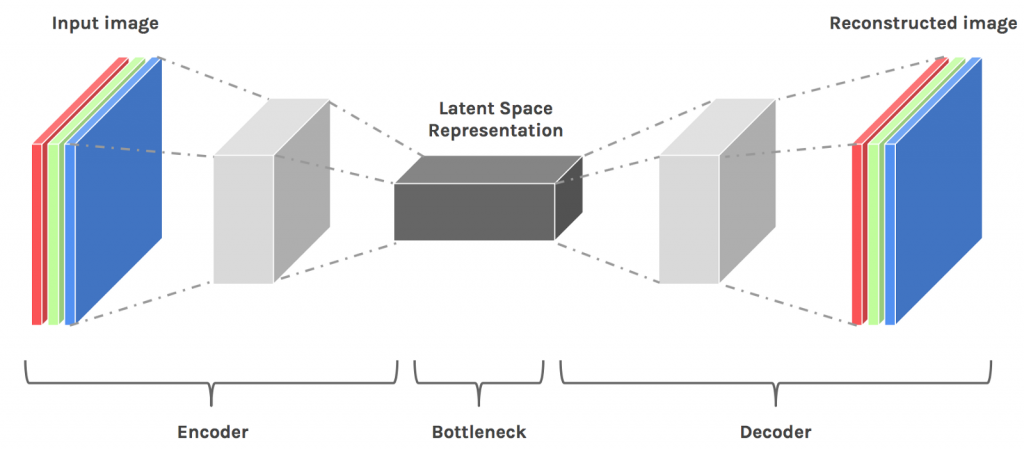
\includegraphics[width=0.8\textwidth]{conv-autoencoder.png}
  \caption{Darstellung eines Convolutional Autoencoders}
\end{figure}


\cite{yt:autoencoder_faces}

\section{Denoising-Autoencoder}
Ein Denoising-Autoencoder oder einfach Denoiser ist ein leicht abgeaenderter
Autoencoder. Er wird verwendet um ein Rauschen aus Bildern zu entfernen.
\para{}
Er unterscheidet sich insofern von dem klassischen Autoencodern, dass er
richtige Labels hat und nicht einfach die Features kopiert. Sein Input stellen
die verrauschten Bilder dar und die Labels sind die unverrauschten Bilder. Somit
wird er darauf trainiert das Rauschen zu entfernen. \\
Man mag sich nun die Frage stellen, weshalb man hierfuer einene Autoencoder und
kein normales CNN verwendet. Empirisch hat sich einfach gezeigt, dass sich
Denoiser dafuer besser eignen. Das hat nachvollziehbare Gruende. Bei der
Entwicklung des Code fuer Encoding-Repraesentation, kann das Rauschen nicht
codiert werden, da es voellig zufaellig ist. Es existieren keine Muster oder
Gesetzmaessigkeiten, welche anderst codiert werden koennten. Somit muss der
Autoencoder diese Rausch-Features verwerfen. Somit hat er leichteres Spiel
gegenueber sonstigen CNNs.
\subsection{Generierung der verrauschten Bilder}



% ------------------------------------

\chapter{Implementation fuer Maschinelles Lernen}
In diesem Kapitel werden wir einige Frameworks betrachten, welche eine
Implementation der ML-Algorithemen realisiert haben. Wir werden sie in ihrer
groben Funktionsweise untersuchen. Diese Tools werden wir im
naechsten Kapitel benutzten um dann ein konkretes Modell zu programmieren.

\section{TensorFlow}
\keyword{TensorFlow}, kurz TF, ist ein von Google entwickeltes \keyword{Framework} fuer
\keyword{datenstromorientriere Programmierung}. Es ist im Grunde genommen eine
Mathematik-Programmbibliothek fuer numerische Berechnungen, dessen Hauptanwendungsbereich im Maschinellen Lernen
liegt. Die Vorteile von TF bestehen vorallem darin, dass die praktische
Anwendung des Frameworks sehr
einfach ist und fast keine mathematische Vorkenntnisse voraussetzt. Somit kann
man sehr einfach ein ML-Modell definieren, trainieren und verwenden. Ausserdem
besitzt TF sehr performante Implementierungen, welche Algorithmen, wie die
Vorwaertspropagierung und die Rueckwaertspropagierung, sehr schnell ausfuehren
laesst. Somit geht das Training von ML-Modellen deutlich schneller als bei
selbstgeschriebenen Implementationen.
TF ist gratis und ein Open-Source-Projekt. Es kann auf Github gefunden werden
unter: https://github.com/tensorflow/tensorflow.
\para{}
In der Industrie ist TensorFlow sehr weit verbreitet. Es wird von den
verschiedensten Unternehmen fuer ihre Anwendungen gebraucht, darunter waren:
Google, Twitter, AirBnB, Intel, CocaCola, Snapchat und noch viele mehr.
\para{}
Grundsaetzlich wurde TF fuer Maschinelles Lernen entwickelt. Speziell eigenet es
sich fuer Deep Learning mit kuenstlichen neuronalen Netzen. Es ist ein
Interface, welches das definieren von Modellen erlaubt, welche dann mit den
eingebauten ML-Algorithmen trainiert werden koennen. \\
Trotz dieser eigentlichen Grundidee von TF, sollten die Abstraktionen eigentlich
fuer beliebige Anwendugen, welche mit numerischen Berechnungen zu tun haben,
sich eignen.
\para{}
Im folgenden werden die grobe Funktionsweise von Tensorflow untersuchen. Um
genau zu sein betrachten wir Tensorflow-Core Version r1.14.
\footnote{Momentan befindet sich TF 2.0 in der Beta. Es ist eine grosse
  Ueberarbeitung des Frameworks. Es ist zu empfehlen, sobald TF 2.0 offiziel
  veroeffentlich wurde, es zu verwenden.}
Wir werden TF nur sehr grob betrachten, da wir spaeter nicht direkt damit
arbeiten werden, sondern mit der High-Level-API Keras. Trotzdem ist er hilfreich
ein grobes Verstaentniss ueber TF zu besitzen.

\para{}
\cite{book:tensorflow}

\subsection{Client und Master}
Wie die meisten grossen Programmbibliotheken ist Tensorflow in Backend und
Fontend aufgeteilt. Das Frontend von Tensorflow bezeichnet man als
\keyword{Client} und das Backend als \keyword{Master}.
\para{}
\begin{infobox}{Fontend und Backend}
  Das \keyword{Frontend} ist der Teil eines Programmes, mit welchem der Benutzer
  interagiert. Es stellt eine Schnittstelle zu dem sogennanten Backend eines
  Programmes dar. Es exponiert so gewisse Funktionalitaeten des Programmes dem
  Benuzter gegenueber, ohne dass er dabei etwas von der zugrundeliegenden Logik mitbekommt.
  \para{}
  Das \keyword{Backend} ist das Gegenstueck zum Frontend. Es implementiert
  jedigliche Programmlogik, welche das gewuenschte Verhalten der Applikation
  hervorruft. Der Benutzer hat keinen direkten Zugriff auf diesen Teil des
  Programmes und bekommt somit nichts von dessen Existenz mit.
\end{infobox}
\para{}
Der Client - also das Frontend - von TF ist in \keyword{Python} geschrieben.
\footnote{
  Tensorflow besitzte mehrere Frontends, welche in den verschiedensten
  Programmiersprachen geschrieben sind. Wir werden jedoch nur das
  Python-Frontend betrachten, da es am besten von TF unterstuetzt ist.
}
Python ist allgemein als eine sehr einsteigerfreundliche Programmiersprache bekannt. Sie
ermoeglicht es dem Benutzer mit wenigen Zeilen Code und ziemlich intuitiv
TensorFlow zu verwenden. Wenn wir also mit TensorFlow programmieren, werden wir
mit Python-Code arbeiten.
\para{}
Der Master - also das Backend - von TF ist dagegen in \keyword{C++} (und CUDA)
geschrieben. Dies hat den Grund, dass C++ im Gegensatz zu Python sehr performant
ist. Also ist die Zeit zum Aufuehren eines Programmes sehr kurz. Dafuer ist der
Programmcode deutlich anspruchsvoller und verboser. Da der Benutzer jedoch keine
direkte Interaktion mit dem Master hat, bekommt er davon nichts mit.

\subsection{Verwendung - der Client}
Nun moechten wir betrachten wie man TensorFlow zu verwenden hat, damit wir
spaeter ein ML-Modell damit basteln koennen. Dafuer werden gewisse
Python-Kenntnisse vorausgesetzt. Wir betrachten nun also
den Client von TF. Man verwendet verschiedene Konzepte um
programmatisch mit TF zu arbeiten. Im folgenden Abschnitt werden wir diese
Konzepte behandeln.

\subsubsection{Graph}
TensorFlow ist datenstromorientiert. Das bedeutet, dass man eine Berechnung
(engl.: computation) durch einen gerichteten Graphen beschreibt. Zuerst stellt
man diesen Graph auf und fuegt ihn zusammen und erst nach der Definition fuehrt man
ihn aus.
Es handelt es sich dabei um einen \keyword{Computation Graph}, wie wir ihn schon in Sektion (\ref{sec:backpropagation}) kennengelernt
haben. In TensorFlow bezeichnet man diesen Graphen als einen \keycode{tf.Graph}.
\para{}
Er besteht aus einer Menge an Knoten, welche miteinander ueber Pfade
verbunden sind. Die Knoten halten Werte in sich, welche ueber die Pfade,
verrechnet werden und in den naechsten Knoten eingespeist werden. Die Pfade sind also die Operationen, welche auf die Werte
angewandt werden. So fuehrt der Graph eine Datenstrom-Berechnung aus.
Jeder Knoten hat null oder mehr Inputs und null oder mehr Outputs.
\para{}
Man muss einen Graph nicht explizit definieren (kann es aber, falls man mehrere
Graphen braucht), da beim defnieren der Operationen sie implizit dem
sogennanten \keyword{Default Graph} hinzugefuegt werden.

\subsubsection{Tensoren}
Die zentrale Dateneinheit in TensorFlow sind Tensoren, wie wir sie bereits in
Sektion (\ref{sec:tensor}) kennengelernt haben.
Auch die Knoten des Graphs reprasentieren Tensoren, welche aber keine feste Wert
enthalten, da sie erst beim Ausfuehren des Graphens, mit Werten befuellt werden.
Nach der Ausfuehrung der Graphs, kann man die Zahlenwerte auslesen.
\para{}
Man verwenet in TF deshalb Tensoren, weil so die Daten beliebige Dimensionalitaeten
und Formen annehmen koennen. Es koennen sowohl Listen von Zahlen (Vektoren),
wie auch Bilder (Tensoren dritter Ordnung) verrechnet werden. \\
Nun sollte auch klar sein, weshalb wir bei der Herleitung der Gleichungen, auch
immer eine Matrixschreibweise erarbeitet haben.
\para{}
In Tensorflow bezeichnet man einen Tensor mit \keycode{tf.Tensor}.
Er ist definiert durch seine Form (Stufe inbegriefen) und den Datentyp seiner
Elemente (z.B. tf.float32).
\para{}
Jeder tf.Tensor ist mit einer einzigen Graph-Ausfuehrung assoziert. Sie
besitzen ihren Wert nur fuer den jeweiligen Durchlauf, danach wird er verworfen.
Man sagt die Tensoren sind ``immutable'', da die Werte nicht erhalten bleiben
und so nicht modifiziert werden koennen.
\para{}
Die soeben beschriebene Tensoren agieren einfach als Durchflussstellen innerhalb
des Graphen. Sie muessen nicht explizit definiert werden, da sie automatisch
eingefuegt werden, wenn der Graph durch seine Operationen definiert wird.
\para{}

Neben dieser Art von Knoten, gibt es noch verschiedene Inputknoten.
stellen den Input in den Graphen dar und muessen explizit definiert werden. Von ihnen gibt es verschiedene Arten,
welche wir nun betrachten werden.

\paragraph{tf.constant}
Der \keycode{tf.Constant} Tensor ist ein Input-Knoten in den Graphen.
Er hat immer einen konstanten Wert als Output. Dieser wird beim Erstellen
angegeben.
\begin{minted}[frame=lines,framesep=2mm,baselinestretch=1.2,bgcolor=lightgray,fontsize=\footnotesize,linenos]{python}
  <Varname> = tf.constant(<Wert>)
\end{minted}
\para{}
Folgender Python-Code ist ein Beispiel, welcher drei konstante Tensoren mit unterschiedenlichen
Formen erstellt. Als Argument, gibt man die Elemente des Tensors, worueber auch
die Form ersichtlich an.
\begin{minted}[frame=lines,framesep=2mm,baselinestretch=1.2,bgcolor=lightgray,fontsize=\footnotesize,linenos]{python}
  skalar = tf.constant(1.0)
  vector2 = tf.constant([1.0, 2.0])
  matrix2x2 = tf.constant([[1.0, 2.0], [3.0, 4.0]])
\end{minted}
\[\text{skalar}=1 \quad \text{vector2}=\begin{pmatrix}1&2\end{pmatrix} \quad
  \text{matrix2x2}=\begin{pmatrix}1&2\\3&4\end{pmatrix}\]

\paragraph{tf.placeholder}
Um den Graphen fuer Maschinelles Lernen zu verwenden, braucht man eine
Moeglichkeit ihn mit Inputs fuer die Modelle zu befuettern. Um dies moeglichst
komfortabel zu machen, gibt es den sogennanten
\keycode{tf.Placeholder} Tensor. Wie der Name es schon sagt, ist er ein
Platzhalter fuer die Inputs, welcher beim Start der Graphausfuehrnug eingespeist
werden. Man muss einzig seine Dimensionen und seinen Datentyp (z.B. tf.float32) bei der Erstellung angeben.
\para{}
\begin{minted}[frame=lines,framesep=2mm,baselinestretch=1.2,bgcolor=lightgray,fontsize=\footnotesize,linenos]{python}
  <Varname> = tf.placeholder(dtype=<Datentyp>, shape=<Form>)
\end{minted}
Fuer den Datentyp waehlt man eigentlich immer
\mintinline{python}{dtype=tf.float32}. Somit kann man mit Gleitkommazahlen rechnen.
Die Form gibt man einfach als $n$-Tupel von Integern an, welche die Anzahl
Komponenten in der jeweiligen Dimension angeben. Somit bedeutet die Form
\mintinline{python}{shape=(4,2,3)} einen Tensor im Tensorraum $\set{R}^{4 \times
  2 \times 3}$.

\paragraph{tf.variable}
Ein weiteres Kriterium um Maschinelles Lernen mit dem tf.Graph durchzufuehren,
ist dass man Modellparameter einfuehren kann. Dafuer ist der
\keycode{tf.Variable} Tensor geeignet. Er ist im Gegensatz zu den anderen
Tensoren ``mutable''. Das bedeutet, dass seine Werte unabhaengig von einer
einzigen Graphenausfuehrung existieren und erhalten bleiben. Seine Elementen
koennen modifiziert werden. Somit sind sie geeignet, fuer Modellparameter.
Die Werte bleiben grundsaetzlich jede Ausfuehrung erhalten und koennen beim
Trainingsdurchlauf angepasst werden.
\para{}
Folgender Python-Code kreirt eine tf.Varaible mit einem Anfangswert und aendert ihren Wert danach.
\begin{minted}[frame=lines,framesep=2mm,baselinestretch=1.2,bgcolor=lightgray,fontsize=\footnotesize,linenos]{python}
  <Varname> = tf.Variable(<Initialwert>, name=<optionaler Name>)
  <Varname>.assign(<neuer Wert>)
\end{minted}
Bei der neuen Wertebesetzung kann auch der alte Wert des Tensors referenziert
werden, um den Wert zum Beispiel zu erhoehen:
\mintinline{python}{var.assign(var + 2.0)}.

\subsubsection{Operationen}
Die Knoten des tf.Graph - also die Tensoren - werden ueber die Pfade aufeinander
abbgebildet. Die Operationen, welche sie aufeinander abbildet, bezeichnet man
als \keycode{tf.Operation}. Eine tf.Operation besitzt jeweils einen Namen und repraesentiert eine
abstrakte Berechnung. Sie hat jeweils null oder mehr Tensor-Objekte als
Input, wie auch als Output.
\para{}
Man definiert meistens keine neuen Operationen, sondern verwendet einfach die vordefinierten.
Ein Beispiel dafuer waere die \keycode{tf.matmul(a,b)}, welche eine
Matrixmultiplikation zwischen \mintinline{python}{a} und \mintinline{python}{b}
ausfuehrt. Im folgenden Code wird das Resulat im neuen Tensor
\mintinline{python}{c} gespeichert.
``MatMul'' bezeichnet).
\begin{minted}[frame=lines,framesep=2mm,baselinestretch=1.2,bgcolor=lightgray,fontsize=\footnotesize,linenos]{python}
  c = tf.matmul(a, b)
\end{minted}
\para{}
Mit diesem Konzept koennen wir nun endlich den eigentlichen Graph definieren.
Dafuer muss man lediglich ein paar Inputtensoren erstellen, und diese mithilfe
von Operationen verrechnen. Natuerlich kann man die Resulate der Operationen
dann weiter verrechnen, bis man den gewuenschten Grapen hat.
\para{}
Hier ein Beispiel eines solchen Graphs.
\begin{minted}[frame=lines,framesep=2mm,baselinestretch=1.2,bgcolor=lightgray,fontsize=\footnotesize,linenos]{python}
  # Inputknoten
  a = tf.constant([[1.0, 2.0], [3.0, 4.0]])
  b = tf.constant([[1.0, 1.0], [0.0, 1.0]])
  # Operationen
  c = tf.matmul(a, b)
  d = tf.placeholder(dtype=tf.float32, shape(2,2))
  e = tf.add(c, e)
\end{minted}

\begin{figure}
  \caption{Visualisierung des beschriebenen \keycode{tf.graph}}
\end{figure}
\para{}


\subsubsection{Session}
Der Client kommuniziert mit dem Master ueber eine sogennante
\keycode{tf.Session}.
Sie ist die Schnittstelle zwischen Frontend und Backend und ermoeglicht es einen tf.Graph
zu erstellen und ihn auszufuehren.
Um die Session zu erstellen verwendet man die Funktion \keycode{tf.Session()}.
\begin{minted}[frame=lines,framesep=2mm,baselinestretch=1.2,bgcolor=lightgray,fontsize=\footnotesize,linenos]{python}
  sess = tf.Session()
\end{minted}
Es ist Best-Practise eine Session, wie eine Datei ueber das
\keycode{with}-Statment zu oeffen und zu schliessen.
\begin{minted}[frame=lines,framesep=2mm,baselinestretch=1.2,bgcolor=lightgray,fontsize=\footnotesize,linenos]{python}
  with tf.Session() as sess:
  # Code
\end{minted}
\para{}
Um den Graphen nun zu berechnen, muss man lediglich die Session ausfuehren, das
geschieht ueber die Methode \keycode{tf.Session.run()}.
Diese Funktion erwartet als Argument einerseits den Knotenpunkt, welchen man
berchnen moechte. Dessen Wert ist der Rueckgabewert der Funktion.
Andererseits erwartet die Funktion noch einen Python-Dictionary, den sogennanten
\keycode{feed\_dict}, welcher die \code{tf.placeholder} mit ihren Werten befuellt.
\begin{minted}[frame=lines,framesep=2mm,baselinestretch=1.2,bgcolor=lightgray,fontsize=\footnotesize,linenos]{python}
  result = sess.run(<Knotenpunkt>, feed_dict=<Placeholder-Dictionary>)
\end{minted}
Es folgt nun ein Codebeispiel, welches die Forwaertspropagierung eines
Sigmoide Neurons mit drei Inputs implementiert. Es wird es mit den Inputs $x = \trans{\begin{pmatrix}1&2&3\end{pmatrix}}$ ausgefuehrt.
\begin{minted}[frame=lines,framesep=2mm,baselinestretch=1.2,bgcolor=lightgray,fontsize=\footnotesize,linenos]{python}
  import tensorflow as tf

  # Inputs
  x = tf.placeholder(dtype=tf.float32, shape=(3))

  # Modellparameter
  w = tf.Variable(tf.random_uniform([3], -1, 1), name='weight')
  b = tf.Variable(tf.random_uniform(1, -1, 1), name='bias')

  # Forwaertspropagierung
  z = tf.add(tf.tensordot(x, w, 1), b)
  a = tf.sigmoid(z)
  y = a

  with tf.Session() as sess:
  res = sess.run(y, feed_dict = {x: [1, 2, 3]})
  print(res)
\end{minted}

\subsubsection{Optimizer}
Um ein ML-Modell in TF zu implementieren, muss man das ganze Modell mit
allen Operationen als Graphen definieren. Dies hoert sich im Moment noch sehr
aufwendig an, ist es jedoch nicht. Wir werden naemlich die High-Level-API Keras
zur Hilfe ziehen, bei der Graphen erstellt.
Keras stellt Implementationen von verschiedenen KNN-Schichten zu verfuegen, damit man sie nicht mehr selber
erstellen muss. Diese kann man dann einfach zu einem Graphen zusammenfuegen.
Aber dazu spaeter mehr.
\para{}
Die Ausfuehrung des erstellen Graphen stellt dann einfach eine
Vorwaertspropagierung dar. Bevor jedoch das Modell brachbare Resualte liert,
muss man es trainieren. Dafuer verwendet man einen \keycode{tf.train.Optimizer}.
\para{}
Der erste Schritt ist dafuer eine Kostenfunktion zu definieren. Es sthene dabei
Verschiedne aus \keycode{tf.losses} zur Verfuegung. Als Argument nimmt die
Kostenfunktion die Label-Tensoren \code{labels} und die Vorhersagen-Tensoren \code{predictions}.
Beispielsweise koennte man den Mittleren Quadratischen Fehler waehlen:
\begin{minted}[frame=lines,framesep=2mm,baselinestretch=1.2,bgcolor=lightgray,fontsize=\footnotesize,linenos]{python}
  cost = tf.losses.mean_squared_error(labels=y_hat, predictions=y)
\end{minted}
Nun erstellt man den Optimizer. Dabei stehen wieder mehrere zur Auswahl. Der
\keycode{tf.train.GraidentDescentOptimizer} ist eine Implementation des
Gradientenverfahren. Er nimmt als Arugment die Lernrate $\eta$.
\begin{minted}[frame=lines,framesep=2mm,baselinestretch=1.2,bgcolor=lightgray,fontsize=\footnotesize,linenos]{python}
  optimizer = tf.train.GradientDescentOptimizer(learning_rate=<>)
\end{minted}
Nun kann man den Optimizer damit beauftragen die Kostenfunktion \code{loss} zu
minimieren. Ausserdem muss man dem Optimizer eine List von \code{tf.Variable}s
geben, welche die zu optimierenden Modellparameter sind.
Man erhaelt so man eine Optimierungs-Operation, welche man dann
ausfuehren kann.
\begin{minted}[frame=lines,framesep=2mm,baselinestretch=1.2,bgcolor=lightgray,fontsize=\footnotesize,linenos]{python}
  opt_op = opt.minimize(cost, var_list=<Hyperparameter-Liste>)
  opt_op.run()
\end{minted}
\para{}
Nun folgt ein kleines Beispielmodell, welches trainiert wird.
\begin{minted}[frame=lines,framesep=2mm,baselinestretch=1.2,bgcolor=lightgray,fontsize=\footnotesize,linenos]{python}
  import tensorflow as tf

  # Inputs
  x = tf.placeholder(dtype=tf.float32, shape=(3))

  # Modellparameter
  w = tf.Variable(tf.random_uniform([3], -1, 1), name='weight')
  b = tf.Variable(tf.random_uniform(1, -1, 1), name='bias')

  # Forwaertspropagierung
  z = tf.add(tf.tensordot(x, w, 1), b)
  a = tf.sigmoid(z)
  y = a

  cost = tf.losses.mean_squared_error(labels=y_true, predictions=y_pred)


  with tf.Session() as sess:
  print(sess.run(cost)) # cost is just another node
  optimizer = tf.train.GradientDescentOptimizer(0.01)
  train = optimizer.minimize()
  res = sess.run(y, feed_dict = {x: [1, 2, 3]})
  print(res)

  # Daten
  x = tf.constant([[1], [2], [3], [4]], dtype=tf.float32)
  y_true = tf.constant([[0], [-1], [-2], [-3]], dtype=tf.float32)

  # Modell
  linear_model = tf.layers.Dense(units=1)
  y_pred = linear_model(x)

  # Evalutaion
  sess = tf.Session()
  init = tf.global_variables_initializer()
  sess.run(init)

  print(sess.run(y_pred))

  # Loss
  loss = tf.losses.mean_squared_error(labels=y_true, predictions=y_pred)

  print(sess.run(loss))


  # Training
  optimizer = tf.train.GradientDescentOptimizer(0.01)
  train = optimizer.minimize(loss)


  for i in range(100):
  _, loss_value = sess.run((train, loss))
  print(loss_value)

\end{minted}


\subsection{Implementation - der Master}
TF ist gerade deshalb sehr attraktiv fuer ML, da es sehr performant (schnell
ausfuehrbar) ist und dadurch die Trainingszeit fuer die Modelle relativ
kurz haltet. Dies wurde durch verschieden Designentscheidungen von TF erreicht.
\para{}
In diesem Abschnitt werden wir grob die zugrundeliegende Implementation von
TensorFlow betrachten - also den Master - und dabei herausfinden weshalb TF so performant ist.
Ausserdem werden wir herausfinden, wie TF ableiten kann.


\subsubsection{Devices}
Die Kernstuecke des Masters sind die verschiedenen \keyword{Devices}, auf
welchen die Berechnungen ausgefuehrt werden. Ein Device ist jedliche Art von
Computerprozessor, auf welchem die Graphen ausfuehrt werden koennen.
Zu diesen Prozessoren gehoeren die CPU (Hauptprozessor) und die GPU (Grafikprozessor).
\footnote{
  Die normale TensorFlow Version ist nicht in der Lage die GPU zu verwenden. Um
  sie verfuegbar zu machen, muss man die GPU Version installieren. Wir werden im folgenden
  von der GPU-Version ausgehen, da sie erhebliche Performance Vorteile gewaehrt.
}
\para{}

Der Master analysiert die verfuegbaren Devices und bewertete sie, bezueglich
ihren Faehigkeiten. Anhand dieser Bewertung entscheidet der Master dann, auf
welchem Device die Berechnugen ausgefuert werden.
\footnote{
  Es ist moeglich die Graphen auf mehreren Devices gleichzeitig auszufuehren und
  so noch schneller die Modelle zu trainieren. Dies ist jedoch erst fuer sehr
  aufwendige Projekte noetig und erfordert ein fortgeschritteneres Versteantniss.
}
Insofern GPUs zur Verfuegung stehen, waehlt TF grundsaetzlich immer diese, da
sie Tensoroperationen deutlich schneller als CPUs verarbeiten koennen.

\subsubsection{Why dataflow}
Reasons:
\begin{itemize}
\item{Parallelism. By using explicit edges to represent dependencies between operations, it is easy for the system to identify operations that can execute in parallel.}
\item{Compilation. TensorFlow's XLA compiler can use the information in your dataflow graph to generate faster code, for example, by fusing together adjacent operations.}
\item{Portability. The dataflow graph is a language-independent representation of the code in your model. You can build a dataflow graph in Python, store it in a SavedModel, and restore it in a C++ program for low-latency inference.}
\end{itemize}

\subsubsection{Performance und Hardwarebeschleunigung}
Nun moechten wir die Gruende fuer die beachtliche Performance von TF erschliessen.
Der erste wichtiger Faktor dabei ist, dass der Master hauptsaechlich in C++
geschrieben ist. C++ ist eine Programmiersprache die sehr nahe am Maschinen-Code
(engl.: low-level) ist. Somit ist der Code sehr hardwarenah und kann so
schneller ausgefuehrt werden. Der Nachteil besteht dafuer darin, dass die Programmiersprache
ziemlich verbos ist. Das bedeutet man braucht viel Code um eine relativ einfach Idee
auszudruecken. Deshalb wurde der Client von TF in Python geschrieben, was
Abhilfe verschafft und so ein relativ einfaches und unverboses Entwickeln ermoeglicht.
\para{}
\para{}
Der andere wichtige Aspekt fuer die Performance ist wohl die sogennante
\keyword{Hardwarebeschleuniging} (engl. Hardware Acceleration), von welcher TF
gebrauch macht. \\
Hardwarebeschleunigung bezeichnet eine Sammlung an Methoden,
bei welchen man spezialisierte Hardware verwendet um rechenintensive Aufgaben
schneller auszufuehren. Die Architektur einer CPU ist zwar so ausgelegt, dass
sie beliebige Aufgaben ausfuehren kann, jedoch meistens nicht besonders
effizient. Deshalb wurden einerseits neue externe Hardwarebausteine, wie die
GPU, welche sich fuer Grafikberechnungen besonders eignet, entwickelt.
Andererseits wurde auch die interne Architektur der CPU so angepasst, dass sie
auch spezielisierte Aufgaben besser meistert.
\para{}
Der Grossteil der Hardwarebeschleunigung wird durch die
\keyword{Parallelisierung} von Operationen erreicht. Dabei spaltet man eine
rechenintensive Aufgabe in viele Teilaufgaben auf, welche gleichzeitig in
gleicher Weise ausgefuehrt werden. Voraussetzung dafuer ist, dass die
Teilaufgaben unabhaengig voneinander bearbeitet werden koennen. \\
Ein typisches Beispiel fuer die Paralleliserbarkeit von Operationen ist die
Matrixmultiplikation. Moechte man eine Matrix $\mat{A} \in \set{R}^{n \times m}$ mit
einer zweiten Matrix $\mat{B} \in \set{R}^{m \times p}$ multiplizieren, muss man
praktisch $m$-mal die gleichen Schritte ausfuehren: Man berechnet jeweils das
Skalarprodukt zwischen der $i$-ten Zeile von $\mat{A}$ und der $i$-ten Spalte
von $\mat{B}$. Alle diese Skalarprodukte haben keinen Einfluss aufeindander und
koennen so unabhaenigig mit der gleichen Prozedur berchnet werden.
\para{}
Allgemein eignen sich Tensoroperatioen fuer Parallelisierung und damit zur Hardwarebeschleunigung.
Nun ist auch ersichtlich, weshalb TensorFlow als Hauptdatentyp Tensoren
verwendet; damit es gebrauch von der Hardwarebeschleunigung machen kann. wir fast alle Gleichungen des Maschinellen

\paragraph{CPU-Beschleunigung}
Die Hardwarebeschleunigung der CPU ist fuer TensorFlow nur von geringfuegiger
Relevanz, da TF sich vorallem fuer GPU-Hardwarebeschleunigung eignet
und dafuer optimiert ist. Ausserdem ist es praktisch unmoeglich die gleiche
Performance von TF mit einer CPU zu erreichen, welche mit einer GPU moeglich ist.
\para{}
Hauptsaechlich parallelisiert TensorFlow mithilfe von der \keyword{SIMD}. SIMD
ist ein Prinzip zur Paralleliserung einer Insturktion fuer mehrere
Dateneinheiten und steht deshalb fuer ``Single Instruction, Multiple Data''.
SIMD umfasst einerseits die spezifische CPU-Architektur und den dazugehoerigen
Befehlssatz, um die Operatioen zu parallelisieren.
Es gibt verschiedene

SSE4.1, SSE4.2, AVX, AVX2, FMA

\paragraph{GPU-Beschleunigung durch cuDNN und CUDA}
cuDNN ist die NVIDIA CUDA Deep Neural Network library. Sie ist eine
GPU-beschleunigte Bibliothek fuer deep neural networks. Sie stellt
implementation fuer standard routines wie Vorwaerts- und Rueckwaertspropagierung bereit.

\subparagraph{CUDA}
\subparagraph{cuDNN}


\subsubsection{Automatische Gradientenberechnung}
Als wir die Rueckwaertsprogagierung hergeleitet haben, haben wir mithilfe von
Computation Graphs die Kettenregel angewandt um die partiellen Ableitungen zu
bilden. Genau das gleiche macht TF, jedoch automatisiert. Aus diesem Grund ist
TF auch datenstromorient.


% Many optimization algorithms including common ml training algorithms like SGD
% compute the gradient of a cost function with respect to a set of inputs.
% Therefor TF has a built-in support for automatic gradient computation.
% It extends the TF Graph using following procedure:
% If TF needs to compute the gradient of a tensor $C$ with respect to some tensor
% $I$ it first finds the path in the computation graph from $I$ to $C$. It then
% backtracks from $C$ to $I$ and for each operation on the backward path it adds a
% node to the graph composing the partial gradients using the chain rule. The
% newely added node computes the gradient function for the corresponding operation
% in the forward path.
% Code: [db,dW,dx] = tf.gradients(C, [b,W,x])


\subsection{Tensorboard}
\subsubsection{Notizen}
TensorBoard is a companion visualitzayion yool for TensorFlow for understanding
the structure of the computation graphs as well as the overall behaviour of the
ML-Modell.

Muss im terminal als Programm gestartet werden: tensorboard --logdir .

\subsubsection{Visualizing computational graphs}
Due to the size and topology of these graphs with maybe over 10'000 nodes the
nodes are groupped and collapsed into high-level blocks. The visualtionsation is
interactive and can pan, zoom and expand.


\begin{minted}[frame=lines,framesep=2mm,baselinestretch=1.2,bgcolor=lightgray,fontsize=\footnotesize,linenos]{python}
  writer = tf.summary.FIleWriter('.')
  writer.add_graph(tf.get_default_graph())
  writer.flush()
\end{minted}

\subsubsection{Visualization of Summary Data/Training}
When training Ml-models users often want to examine the state of various aspect
of the model and how they change over time. In this way the can observe the
learning behaviour of the model, whetever or not it converges and how fast it
does this. With this informations the best hyper parameters can be chosen. The
operations used to compute these summarisations are then inserted into the
TF.graph. Interesting values to examine are value of the loss function or the
time taken to execute the graph, histogrambased summaries. The data for
TensorBoard is written by TensorFlow in a log file, which then can be read by
the TensorBoard program. The tensorboard starts a http server and shows the data
in a web browser.


\subsubsection{Visualization of Training}

\section{Keras}
\keyword{Keras} ist ein Open-Source Deep-Learning Framework geschrieben in
Python. Keras wurde entwickelt, um eine einheitliche Schnittstelle fuer
verschieden Backends, wie TensorFlow, Microsoft Cognitive Toolkit und Theano zu
bieten. Seit TF Version 1.4 ist Keras ein fester Bestandteil der TensorFlow-Core-API.

Keras ermoeglicht ein sehr simples und benutzerfreundliches defnieren von
Deep-Learning-Modeln welche dann sehr einfach trainiert werden koennen.
Wir werden also anstatt TF direkt zu verwenden, ueber Keras das Modell definieren.
Deshalb ist ein tiefgehendes Verstaetniss von TF ueberfluessig.

\subsection{Grundsaetliche Funktionsweise}
In Keras ist es sehr einfach ein Modell zu bauen. Man reiht lediglich
vordefinierte KNN-Schichten aneinander und baut so einen Graphen. Dafuer
verwendet man meistens den \code{tf.keras.Sequential} Modus.

\subsection{Schichten}
Keras ist hat verschiedene Schichten von Kuenstlichen Neuronalen Netzen
implementiert. Dies koennen also einfach in den tf.Graph eingefuegt werden.
Wir werden nun diese verschieden Schichten betrachten.

\paragraph{Sequential-Modell/Dense-Layer}
To build a simple, fully-connected network (i.e. multi-layer perceptron):
\begin{minted}[frame=lines,framesep=2mm,baselinestretch=1.2,bgcolor=lightgray,fontsize=\footnotesize,linenos]{python}
  model = tf.keras.Sequential()
  # Adds a densely-connected layer with 64 units to the model:
  model.add(layers.Dense(64, activation='relu'))
  # Add another:
  model.add(layers.Dense(64, activation='relu'))
  # Add a softmax layer with 10 output units:
  model.add(layers.Dense(10, activation='softmax'))
\end{minted}


\paragraph{Configure the layers}

There are many tf.keras.layers available with some common constructor parameters:

activation: Set the activation function for the layer. This parameter is specified by the name of a built-in function or as a callable object. By default, no activation is applied.
kernelinitializer and biasinitializer: The initialization schemes that create the layer's weights (kernel and bias). This parameter is a name or a callable object. This defaults to the "Glorot uniform" initializer.
kernelregularizer and biasregularizer: The regularization schemes that apply the layer's weights (kernel and bias), such as L1 or L2 regularization. By default, no regularization is applied.


\begin{minted}[frame=lines,framesep=2mm,baselinestretch=1.2,bgcolor=lightgray,fontsize=\footnotesize,linenos]{python}
  # Create a sigmoid layer:
  layers.Dense(64, activation='sigmoid')
  # Or:
  layers.Dense(64, activation=tf.sigmoid)

  # A linear layer with L1 regularization of factor 0.01 applied to the kernel matrix:
  layers.Dense(64, kernel_regularizer=tf.keras.regularizers.l1(0.01))

  # A linear layer with L2 regularization of factor 0.01 applied to the bias vector:
  layers.Dense(64, bias_regularizer=tf.keras.regularizers.l2(0.01))

  # A linear layer with a kernel initialized to a random orthogonal matrix:
  layers.Dense(64, kernel_initializer='orthogonal')

  # A linear layer with a bias vector initialized to 2.0s:
  layers.Dense(64, bias_initializer=tf.keras.initializers.constant(2.0))

\end{minted}


\paragraph{Conv2D}

\paragraph{MaxPooling2D}
\paragraph{UpSampling2D}

\subsection{Train and evaluate}

Train and evaluate
Set up training

After the model is constructed, configure its learning process by calling the compile method:

\begin{minted}[frame=lines,framesep=2mm,baselinestretch=1.2,bgcolor=lightgray,fontsize=\footnotesize,linenos]{python}
  model = tf.keras.Sequential([
  # Adds a densely-connected layer with 64 units to the model:
  layers.Dense(64, activation='relu', input_shape=(32,)),
  # Add another:
  layers.Dense(64, activation='relu'),
  # Add a softmax layer with 10 output units:
  layers.Dense(10, activation='softmax')])

  model.compile(optimizer=tf.train.AdamOptimizer(0.001),
  loss='categorical_crossentropy',
  metrics=['accuracy'])

\end{minted}

tf.keras.Model.compile takes three important arguments:

optimizer: This object specifies the training procedure. Pass it optimizer instances from the tf.train module, such as tf.train.AdamOptimizer, tf.train.RMSPropOptimizer, or tf.train.GradientDescentOptimizer.
loss: The function to minimize during optimization. Common choices include mean square error (mse), categorical crossentropy, and binary crossentropy. Loss functions are specified by name or by passing a callable object from the tf.keras.losses module.
metrics: Used to monitor training. These are string names or callables from the tf.keras.metrics module.
\para{}
The following shows a few examples of configuring a model for training:
\begin{minted}[frame=lines,framesep=2mm,baselinestretch=1.2,bgcolor=lightgray,fontsize=\footnotesize,linenos]{python}
  # Configure a model for mean-squared error regression.
  model.compile(optimizer=tf.train.AdamOptimizer(0.01),
  loss='mse',       # mean squared error
  metrics=['mae'])  # mean absolute error

  # Configure a model for categorical classification.
  model.compile(optimizer=tf.train.RMSPropOptimizer(0.01),
  loss=tf.keras.losses.categorical_crossentropy,
  metrics=[tf.keras.metrics.categorical_accuracy])

\end{minted}

\subsubsection{Fit}
Input NumPy data
For small datasets, use in-memory NumPy arrays to train and evaluate a model. The model is "fit" to the training data using the fit method:

\begin{minted}[frame=lines,framesep=2mm,baselinestretch=1.2,bgcolor=lightgray,fontsize=\footnotesize,linenos]{python}
  import numpy as np

  def random_one_hot_labels(shape):
  n, n_class = shape
  classes = np.random.randint(0, n_class, n)
  labels = np.zeros((n, n_class))
  labels[np.arange(n), classes] = 1
  return labels

  data = np.random.random((1000, 32))
  labels = random_one_hot_labels((1000, 10))

  model.fit(data, labels, epochs=10, batch_size=32)

\end{minted}

tf.keras.Model.fit takes three important arguments:

epochs: Training is structured into epochs. An epoch is one iteration over the entire input data (this is done in smaller batches).
batch size: When passed NumPy data, the model slices the data into smaller batches and iterates over these batches during training. This integer specifies the size of each batch. Be aware that the last batch may be smaller if the total number of samples is not divisible by the batch size.
validation data: When prototyping a model, you want to easily monitor its performance on some validation data. Passing this argument—a tuple of inputs and labels—allows the model to display the loss and metrics in inference mode for the passed data, at the end of each epoch.

\subsubsection{Predict}
The tf.keras.Model.evaluate and tf.keras.Model.predict methods can use NumPy data and a tf.data.Dataset.

To evaluate the inference-mode loss and metrics for the data provided:
\begin{minted}[frame=lines,framesep=2mm,baselinestretch=1.2,bgcolor=lightgray,fontsize=\footnotesize,linenos]{python}

  data = np.random.random((1000, 32))
  labels = random one hot labels((1000, 10))

  model.evaluate(data, labels, batch size=32)

  model.evaluate(dataset, steps=30)


  And to predict the output of the last layer in inference for the data provided, as a NumPy array:

  result = model.predict(data, batch size=32)
  print(result.shape)
\end{minted}

\subsection{Weiss nit}

\begin{minted}[frame=lines,framesep=2mm,baselinestretch=1.2,bgcolor=lightgray,fontsize=\footnotesize,linenos]{python}
  inputs = tf.keras.Input(shape=(32,))  # Returns a placeholder tensor

  # A layer instance is callable on a tensor, and returns a tensor.
  x = layers.Dense(64, activation='relu')(inputs)
  x = layers.Dense(64, activation='relu')(x)

  predictions = layers.Dense(10, activation='softmax')(x)

  Instantiate the model given inputs and outputs.

  model = tf.keras.Model(inputs=inputs, outputs=predictions)

  # The compile step specifies the training configuration.
  model.compile(optimizer=tf.train.RMSPropOptimizer(0.001),
  loss='categorical_crossentropy',
  metrics=['accuracy'])

  # Trains for 5 epochs
  model.fit(data, labels, batch_size=32, epochs=5)
\end{minted}


% ------------------------------------

\chapter{Entwicklung eines Denoising-Autoencoders}
Nun sind wir in dem Kapitel angelangt, in welchem das ganze erarbeitete Wissen
zusammenfliesst. Wir werden ein konkretes Machine-Learning-Modell in TensorFlow
zusammen mit Keras programmieren. Dabei wird darauf eingegangen, welche Schritte die
Entwicklung eines solchen Modells umfasst und wie dabei am besten vorgegangen
wird.

\section{Das konkrete Modell}
Als konkretes Modell werden wir einen Convolutional-Denoising-Autoencoder,
dessen Theorie wir bereits behandelt haben, programmieren.
Wir werden ihn verwenden um das Bildrauschen von Bildern wegzurechnen und sie so
wieder erkenntlich zu machen. Als
Bilder werden wir handgeschriebene Ziffern vom MNIST-Datenset verwenden.

\begin{figure}
  \caption{grobes Schema des Modells}
\end{figure}

\para{}
\subsection{Daten}
Als Trainingsdaten verwenden wir den \keyword{MNIST}-Datensatz. Er ist der wohl
bekannteste Datensatz fuer beispielhaftes Maschinelles Lernen.
Er besteht aus schwarz-weiss Bildern von handgeschrieben Ziffern.
Zuesaetzlich gaebe es auch noch Labels zu den Ziffern, da das Modell meistens
fuer Ziffernerkennung trainiert wird. Jedoch werden
wir diese nicht brauchen, da wir einen Autoencoder trainieren.
\para{}
Der Datensatz besteht aus einem Trainingsdatensatz von 60'000 Sampels und einem Testdatensatz
von 10'000 Sampels. Alle Ziffern wurden in soefern schon korrekt formatiert,
dass ihre Groesse auf $28 \times 28$ Pixel normalisiert wurde und sie im Bild
zentriert sind.

\begin{figure}
  \centering
  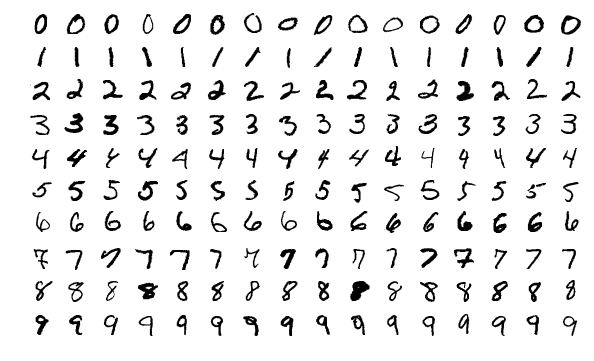
\includegraphics[width=0.7\textwidth]{mnist.png}
  \caption{ein Auszug an MNIST-Bildern \cite{res:mnist_images}}
\end{figure}

\para{}
\cite{net:mnist}

\section{Setup}
Zuallererst muessen wir unser Entwicklungsumfeld richtig konfigurieren. Das
bedeutet, dass wir Python zusammen mit den verschiedenen Programmbibliotheken
installieren muessen.
\para{}
Die Installationsschritte werden in dieser Arbeit fuer eine arch-basierte
Linuxdistribution, welche den \keyword{Pacman}-Package-Manager verwendet, erklaert.

\paragraph{Python3}
Um TensorFlow und Keras verwenden zu koennen, muss Python3 installiert sein.

Um Python3 mithilfe von Pacman zu installieren, muss man folgenden Befehl in
der Kommandozeile ausfuehren.
\begin{minted}[frame=lines,framesep=2mm,baselinestretch=1.2,bgcolor=lightgray,fontsize=\footnotesize]{bash}
  sudo pacman -S python
\end{minted}

\paragraph{Python-Module}
Wir werden fuer unser Python-Programm von zwei Packages Gebrauch machen, welche
nicht in der Standardbibliothek von Python enthalten sind:
\begin{itemize}
\item{NumPy: Ein Package welches verschiedene Mathematische Konzepte
    implementiert; vorallem Vektor- und Matrix-Arithmetik}
\item{Matplotlib: Ein Package zum erstellen von Plots und Grafiken}
\end{itemize}

Man installiert beide mit folgenden Kommandos.
\begin{minted}[frame=lines,framesep=2mm,baselinestretch=1.2,bgcolor=lightgray,fontsize=\footnotesize]{bash}
  sudo pacman -S python-numpy
  sudo pacman -S python-matplotlib
\end{minted}

Nun muessen wir CUDA installieren, damit wir TensorFlow auf der GPU ausfuehren koennen.
\paragraph{CUDA}
\begin{minted}[frame=lines,framesep=2mm,baselinestretch=1.2,bgcolor=lightgray,fontsize=\footnotesize]{bash}
  sudo pacman -S cuda
\end{minted}

Da wir nun CUDA installiert haben, koennen wir auch cuDNN installieren, das
Deep-Learning-Framework fuer CUDA.
\paragraph{cuDNN}
\begin{minted}[frame=lines,framesep=2mm,baselinestretch=1.2,bgcolor=lightgray,fontsize=\footnotesize]{bash}
  sudo pacman -S cudnn
\end{minted}

Zu guter letzt installieren wir noch die GPU-version von TensorFlow mithilfe
folgenden Kommandos.
\paragraph{TensorFlow}
\begin{minted}[frame=lines,framesep=2mm,baselinestretch=1.2,bgcolor=lightgray,fontsize=\footnotesize]{bash}
  sudo pacman -S tensorflow-cuda
\end{minted}


\section{Entwicklung}
Nun beginnen wir mit der eigentlichen Programmierung.

\subsection{Testprogramm}
Zuallerst werden wir ein kleines Testprogramm schreiben, welches ueberprueft, ob
alle Programmabhaengigkeiten korrekt installiert wurden und verwendet werden koennen.

In den ersten Zeilen des Pythonprogamms werden wir die Importstatments
schreiben, um NumPy, Matplotlib und TensorFlow verfuegbar zu machen.
Keras muss nicht explizit geladen werden, da es in TensorFlow drin steckt.
Dann schreiben wir die Versionnummern der verschiedenen Programmbibliotheken
in die Konsole und koennen so ueberpruefen, ob alles richtig konfiguriert ist.
\begin{minted}[frame=lines,framesep=2mm,baselinestretch=1.2,bgcolor=lightgray,fontsize=\footnotesize,linenos]{python}
  import numpy as np # NumPy wird impotiert
  import matplotlib as mpl # Matplotlib wird impotiert

  import tensorflow as tf # TensorFlow wird impotiert

  print(np.__version__) # Schreibt die NumPy-Version nach stdout.
  print(mpl.__version__) # Schreibt die Matplotlib-Version nach stdout.
  print(tf.__version__) # Schreibt die TensorFlow-Version nach stdout.
\end{minted}
Falls der Output folgenden Charakter hat (die Versionsnummern muessen nicht
die gleichen sein) und keine Fehlermeldungen angezeigt
werden, sollte alles funktionieren.
\begin{minted}[frame=lines,framesep=2mm,baselinestretch=1.2,bgcolor=lightgray,fontsize=\footnotesize,linenos]{text}
  1.17.
  3.1.1
  1.14.0
\end{minted}
\para{}

\subsection{Trainingsdaten}
Da wir nun verfiziert haben, dass alle Programmabhaengigkeiten funktionieren,
koennen wir mit dem eigentlichen Programm beginnen.
\para{}
Im den folgenden Auschnitten werden wir den Code immer weiter ausbauen und dabei
erfahren, was er bewirkt. Wir beginnen unser eigentlichens Programm mit folgenden Importstatments.
\begin{minted}[frame=lines,framesep=2mm,baselinestretch=1.2,bgcolor=lightgray,fontsize=\footnotesize,linenos]{python}
  import numpy as np
  import matplotlib.pyplot as plt
  import tensorflow as tf
\end{minted}

\subsubsection{Laden des MNIST-Datensatzes}
Der nun erste Schritt besteht darin, die Datensaetze zu laden. Wie bereits
erwaehnt, werden wir den MNIST-Datensatz verwendet. Da dieser dermassen bekannt
ist, gibt es eine Funktion in Keras, welche automatisch die Daten herunterlaedt
und sie als NumPy Arrays zurueckgibt. Die Funktion gibt die verschiedenen
Komponenten der Daten in folgendem Format zurueck \code{(x\_train, y\_train),
  (x\_test, y\_test)}. Da wir nur an den Features \code{x} interessiert sind,
verwerfen wir die Labels \code{y} einfach mithilfe der Wegwerf-Variabel \code{\_}.
\begin{minted}[frame=lines,framesep=2mm,baselinestretch=1.2,bgcolor=lightgray,fontsize=\footnotesize,linenos]{python}
  (x_train, _), (x_test, _) = tf.keras.datasets.mnists.load_data()
\end{minted}
Nun sind die Features fuers Training in der Variabel \code{x\_train} und die
Features des Trainingsdatensatzes in der Variabel \code{x\_test} gespeichert.

\subsubsection{Formatieren der Daten}
Nun muessen wir die Daten transformieren, damit sie die richtige Form fuer
unser Modell haben. Wie bereits erklaert, ist der MNIST-Datensatz ziemlich
handsam, da die Bilder alle die gleichen Masse haben und die Ziffern zentriert sind.
\para{}
Wir muessen die Grauwerte normalisieren, denn im Moment liegen sie noch
im Intervall $[0, 255]$ und sind vom Typ Integer. Unser Modell kann am besten
mit Kommazahlen im Intervall $[0,1]$ umgehen. Um diese Anpassung vorzunehmen
brauchen wir folgenden Code.
\begin{minted}[frame=lines,framesep=2mm,baselinestretch=1.2,bgcolor=lightgray,fontsize=\footnotesize,linenos]{python}
  x_train = x_train.astype('float32') / 255.0 # Normalisierung
  x_test = x_test.astype('float32') / 255.0 # Normalisierung
\end{minted}
Desweiteren werden wir in unserem Modell ConvLayers verwenden. Diese in Keras
implementieren ConvLayers erwarten die Inputs in der Form $(m, w, h, c)$, wobei
$m$ die Anzahl Bilder ist, $w$ die Bildbreite, $h$ die Bildhoehe und $c$ die
Anzahl Farbkomponenten. Wir formen nun mithilfe von NumPy das Array um.
\begin{minted}[frame=lines,framesep=2mm,baselinestretch=1.2,bgcolor=lightgray,fontsize=\footnotesize,linenos]{python}
  x_train = np.reshape(x_train, (len(x_train), 28, 28, 1)) # neue Form: (60'000, 28, 28, 1)
  x_test = np.reshape(x_test, (len(x_test), 28, 28, 1)) # neue Form: (10'000, 28, 28, 1)
\end{minted}
Nun besitzen die Daten die richtige Form fuer unser Modell.

\subsubsection{Generieren der verrauschten Bilder}
Den Input in unser Modell stellen nicht die normalen MNIST-Bilder dar, sondern
eine verrauschte Variante von ihnen. Diese werden wir nun generieren mithilfe
von additivem Gauss'schem Rauschen.
\para{}
Zuerst erstellen wir eine Matrix $\mat{R} \in \set{R}^{28 \times 28 \times 1}$, welche die gleiche Form, wie die
Bilder hat. Diese Matrix befuellen wir mit Zufallswerten. Fuer die
Zufallswerte verwenden wir eine Gauss'sche Normalverteilung
$\mathcal{N}(\mu = 0, \sigma^2 = 1)$ mit Erwartungswert $\mu = 0$ und Varianz
$\sigma^2 = 1$. Da wir fuer jedes Bild eine eigene Rauschmatrix brauchen,
generieren wir eine Liste $(\mat{R}_1,\mat{R}_2,\ldots,\mat{R}_m$) der Laenge $m$ an
Rauschmatrizen. Dafuer verwenden wir die NumPy Funktion
\code{np.random.normal(loc=<$\mu$>, scale=<$\sigma^2$>,size=<Form>)}.
Die somit erhaltenen Rauschmatrizen multiplizieren wir dann mit einer
Rauschkonstane \code{noise\_factor} und addieren das Resulat auf die MNIST-Bilder.
Nach dem Hinzufuegen der Rauschwerte, muessen wir die Grauwerte noch auf das Intervall
$[0,1]$ kappen. Dafuer verwenden wir die NumPy-Funktion \code{np.clip(var, min, max)}. Diese Schritte wenden
wir sowohl auf den Trainingsdatensatz, wie auch auf den Testdatensatz an. \\
Somit lautet unser Code:
\begin{minted}[frame=lines,framesep=2mm,baselinestretch=1.2,bgcolor=lightgray,fontsize=\footnotesize,linenos]{python}
  noise_factor = 0.5

  # fuer x_train
  noise_matrices = np.random.normal(loc=0.0, scale=1.0, size=x_train.shape)
  noise_matrices *= noise_factor
  x_train_noisy = x_train + noise_matrices
  x_train_noisy = np.clip(x_train_noisy, 0.0, 1.0)

  # fuer x_test in Kurzfassung
  x_test_noisy = x_test + noise_factor * np.random.normal(loc=0.0, scale=1.0, size=x_test.shape)
  x_test_noisy = np.clip(x_test_noisy, 0.0, 1.0)
\end{minted}
\para{}
Wir koennen mithilfe der Matplotlib einen Blick auf die verrauschten Bilder
neben den Originalbildern werfen. Wir erstellen einfach einen Plot, welcher
jeweils 10 Bilder beider Arrays rendert.
\begin{minted}[frame=lines,framesep=2mm,baselinestretch=1.2,bgcolor=lightgray,fontsize=\footnotesize,linenos]{python}
  n = 10 # jeweils 10 Bilder
  plt.figure()
  for i in range(n):
    # verrauschte Bilder
    ax = plt.subplot(2,n,i+1+n)
    plt.imshow(x_test[i].reshape(28,28))
    plt.gray()

    # Original Bilder
    ax = plt.subplot(2, n, i+1)
    plt.imshow(x_test_noisy[i].reshape(28,28))
    plt.gray()

  plt.show()
\end{minted}
Wir erhalten so folgende Grafik:
\begin{figure}[h!]
  \centering
  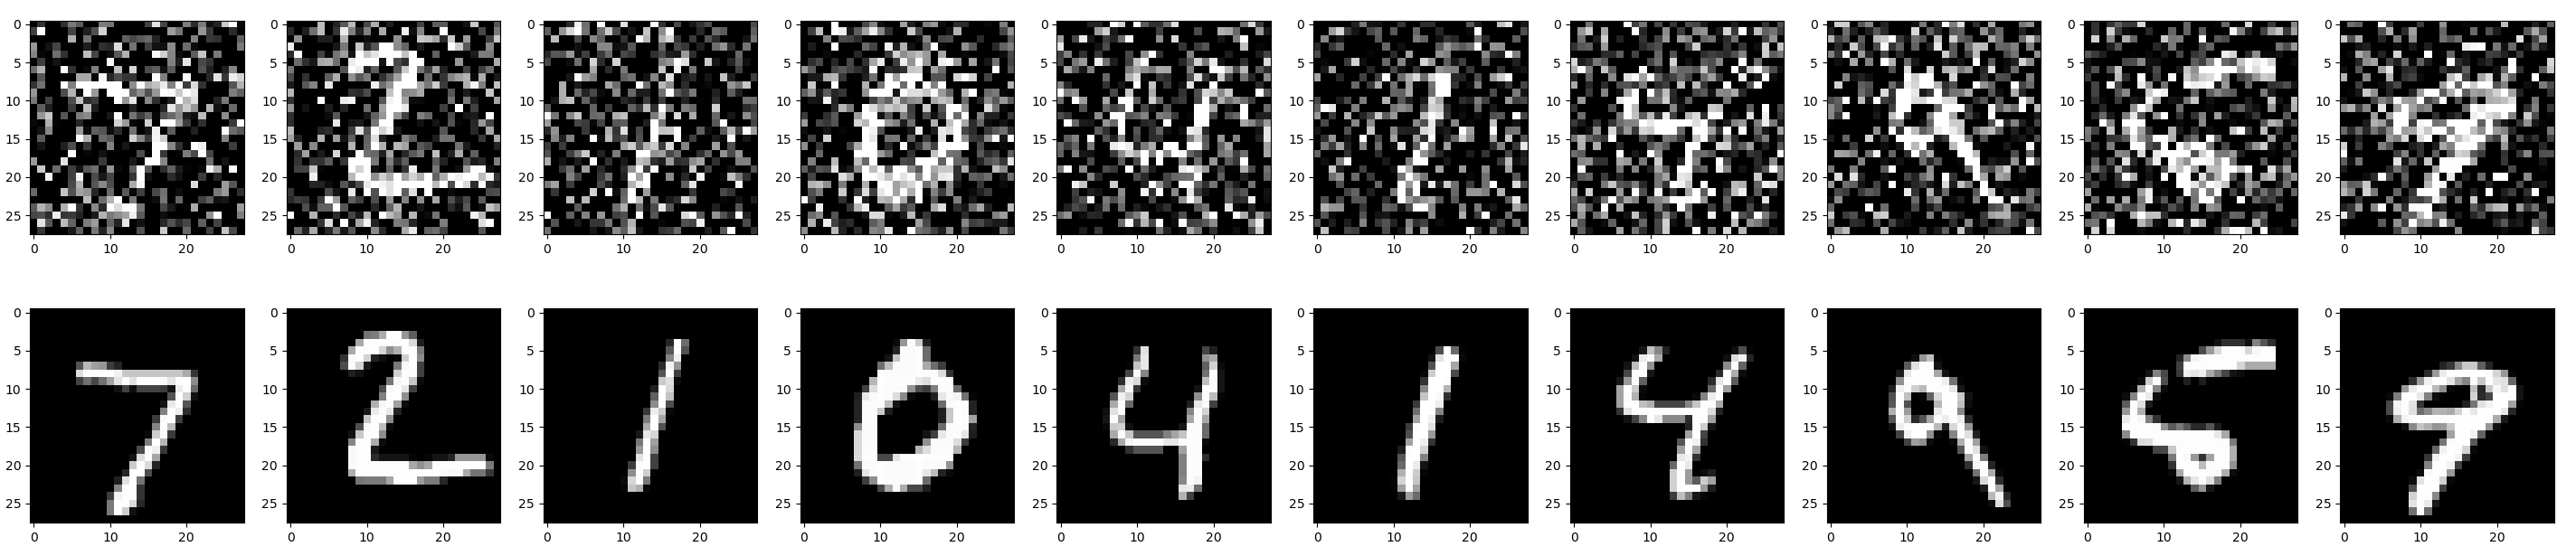
\includegraphics[width=0.9\textwidth]{noised_clipped.png}
  \caption{Verrauschte Bilder neben den Orignalbildern}
\end{figure}

\para{}
Nun haben wir die Daten vollstaendigt im richtigem Format. Damit koennen wir nun
zur Definition des Modells uebergehen.



\subsection{Modell definieren}
Nun werden wir mithilfe von Keras das Modell unseres
Convolutional-Denoising-Autoencoders definieren.
Wir werden das Modell nach dem Vorbild der Theorie bauen.
Wie wir wissen umfasst die Topologie eines CNNs die verschiedentsten
Hyperparameter. Wir werden der einfachheitshalber vorerst unbegruendete Werte
dafuer waehlen. Spaeter werden wir diese Hyperparameter noch einstellen.
\para{}
Wir beginnen unser Modell mit der Inputsschicht $l=0$, welche einfach ein Tensor
ist, welcher die Inputswerte haelt. Die Schicht hat die gleiche Form, wie ein MNIST-Bild.
\begin{minted}[frame=lines,framesep=2mm,baselinestretch=1.2,bgcolor=lightgray,fontsize=\footnotesize,linenos]{python}
  input_data = tf.keras.Input(shape=(28,28,1))
\end{minted}
\para{}
Nach dieser Inputschicht folgt der Encoder des Autoencoders. Dieser besteht
sowohl aus Convolutional-Schichten, wie auch aus Pooling-Schichten, welche sich abwechseln.
Wir werden wie gesagt fuer alle Schichten vorerst die gleichen unbegruendeten
Hyperparameter waehlen. Fuer die Convolutional-Schichten waehlen wir
eine Filtergroesse $f^l = 3$, eine Anzahl Filter von $c^l = 32$,
einen Stride $s=1$, Same-Padding und die ReLU-Aktivierungsfunktion $\varphi = \varphi^{\text{ReLU}}$.
Der Code fuer die Defition einer solchen Convolutional-Schicht lautet:
\begin{minted}[frame=lines,framesep=2mm,baselinestretch=1.2,bgcolor=lightgray,fontsize=\footnotesize,linenos]{python}
  conv_layer = tf.keras.layers.Conv2D(filters=32, kernel_size=(3,3),
  strides=(1,1),padding='same', activation='relu')(input_data)
\end{minted}
Fuer die Pooling-Schichten waehlen wir analog eine Feldgroesse $f = 2$, einen
Stride $s = 2$, damit jedes Feld einmal zusammengefasst wird und Same-Padding.
Der Code fuer eine dieser Pooling-Schichten lautet:
\begin{minted}[frame=lines,framesep=2mm,baselinestretch=1.2,bgcolor=lightgray,fontsize=\footnotesize,linenos]{python}
  pool_layer = tf.keras.layers.MaxPooling2D(pool_size=(2,2),strides=(2,2),padding='same')(econv0)
\end{minted}
Nun folgt der Decoder.
Fuer ihn verwenden wir die gleichen Convolutional-Schichten wie im Encoder. Anstatt
Pooling-Schichten enthaelt er UpSampling-Schichten, bei welchen die
Feldgroesse $f = 2$ gewaehlt wurde. Somit werden $4 \times 4$-Felder zu einem
einzigen Pixel zusammengefasst. Als Interpolationsmethode benutzten wir den Naechsten-Nachbar-Algorithmus.
Eine solche UpSampling-Schicht definiert man also so:
\begin{minted}[frame=lines,framesep=2mm,baselinestretch=1.2,bgcolor=lightgray,fontsize=\footnotesize,linenos]{python}
  dupsample0 = tf.keras.layers.UpSampling2D(size=(2,2), interpolation='nearest')(dconv0)
\end{minted}
Wir definieren jetzt alle Schichten und verknuepfen sie miteinander. Wir bauen
einen Autoencoder, dessen Flaschenhals zwei Convolutional-Schichten tief ist.
Somit besteht der Encoder aus zwei Convolutional-Layer-Pooling-Layer-Paar, dann
folgt der Flaschenhals und aus zwei Convolutional-Layer-UpSampling-Layer-Paar.
Der ganze Graph wird durch folgenden Code gebildet:
\begin{minted}[frame=lines,framesep=2mm,baselinestretch=1.2,bgcolor=lightgray,fontsize=\footnotesize,linenos]{python}
  econv0 = tf.keras.layers.Conv2D(filters=32, kernel_size=(3,3), strides=(1,1),padding='same',activation='relu')(input_data)
  emaxpool0 = tf.keras.layers.MaxPooling2D(pool_size=(2,2),strides=None,padding='same')(econv0)
  econv1 = tf.keras.layers.Conv2D(filters=32, kernel_size=(3,3), strides=(1,1),padding='same',activation='relu')(emaxpool0)
  emaxpool1 = tf.keras.layers.MaxPooling2D(pool_size=(2,2), strides=None,padding='same')(econv1)
  encoded =  emaxpool1 # Flaschenhals der Form (7,7,32)
  dconv0 = tf.keras.layers.Conv2D(filters=32, kernel_size=(3,3), strides=(1,1), padding='same', activation='relu')(encoded)
  dupsample0 = tf.keras.layers.UpSampling2D(size=(2,2), interpolation='nearest')(dconv0)
  dconv1 = tf.keras.layers.Conv2D(filters=32, kernel_size=(3,3), strides=(1,1), padding='same', activation='relu')(dupsample0)
  dupsample1 = tf.keras.layers.UpSampling2D(size=(2,2), interpolation='nearest')(dconv1)
  dconv2 = tf.keras.layers.Conv2D(filters=1,kernel_size=(3,3), strides=(1,1), padding='same', activation='sigmoid')(dupsample1)
  decoded = dconv2
\end{minted}
Wie im Code zu sehen, haben wir fuer alle Convolutional-Layers die ReLU
Aktivierungsfunktion gewaehlt, ausser der letzten Schicht. Fuer die letzte
Schicht gebauren wir die Sigmoid-Aktivierungsfunktion. Dies hat den Grund, dass
der Output unseres Netzwerk wieder ein Bild sein muss, dessen Grauwerte im
Invervall $[0,1]$ liegen muessen. Eine Sigmoidfunktion hat genau dieses
Intervall als Wertemenge.
\para{}
Nun muessen wir noch das Kerasmodell mit diesem Graphen definieren. Also
definieren wir das Modell einfach als der Abschnitt des Graphen zwischen der
Input und dem Decoding.
Und es danach mit kompilieren. Bei der Kompilierung wahlen wir als
Optimierungsverfahren einfach das Stochastische-Gradientenverfahren SGD. Als
Kostenfunktion waehlen wir den Mittleren-Quadratischen-Fehler $C_{\text{MSE}}$.
\begin{minted}[frame=lines,framesep=2mm,baselinestretch=1.2,bgcolor=lightgray,fontsize=\footnotesize,linenos]{python}
  autoencoder = tf.keras.Model(input_data, decoded)
  autoencoder.compile(optimizer='sgd',loss='mean_squared_error') # SGD und MSE
\end{minted}
Mithilfe von \code{tf.keras.Model.summary} kann man eine Zusammenfassung des
Modells in Textform erhalten. So kann man Informationen bezueglich der Form der
verschiedenen Schichten extrahieren und ueberpruefen, ob alles stimmig ist.
Fuer unser Modell erhalten wir folgende Summary:
\begin{minted}[frame=lines,framesep=2mm,baselinestretch=1.2,bgcolor=lightgray,fontsize=\footnotesize,linenos]{text}
Model: "model"
_________________________________________________________________
Layer (type)                 Output Shape              Param #
=================================================================
input_1 (InputLayer)         [(None, 28, 28, 1)]       0
_________________________________________________________________
conv2d (Conv2D)              (None, 28, 28, 32)        320
_________________________________________________________________
max_pooling2d (MaxPooling2D) (None, 14, 14, 32)        0
_________________________________________________________________
conv2d_1 (Conv2D)            (None, 14, 14, 32)        9248
_________________________________________________________________
max_pooling2d_1 (MaxPooling2 (None, 7, 7, 32)          0
_________________________________________________________________
conv2d_2 (Conv2D)            (None, 7, 7, 32)          9248
_________________________________________________________________
up_sampling2d (UpSampling2D) (None, 14, 14, 32)        0
_________________________________________________________________
conv2d_3 (Conv2D)            (None, 14, 14, 32)        9248
_________________________________________________________________
up_sampling2d_1 (UpSampling2 (None, 28, 28, 32)        0
_________________________________________________________________
conv2d_4 (Conv2D)            (None, 28, 28, 1)         289
=================================================================
Total params: 28,353
Trainable params: 28,353
Non-trainable params: 0
_________________________________________________________________
\end{minted}

\subsection{Training}
Nun muessen wir das definierte Modell trainieren.
Mit Keras ist das mit einem Funktionsaufruf gemacht. Diese Funktion erwartet
einige Argumente. Zuerst muessen wir die Features und die Labels angeben. Die
Features haben wir in der Variabel \code{x\_train\_noisy} gespeichert. Die Labels
sind die unverrauschten MNIST-Bilder, welche in Variable \code{x\_train} sind.
Desweiteren spezifizieren wir die groesse eines Mini-Batches als 128. Wir werden
fuer 100 Epochen trainieren und geben dies entsprechend an. Wichtig ist auch,
dass wir die Trainingssampels vor dem Training mischen, damit keine Mustern
innerhalb der Anordnung der Samples erlernt werden. Als letzen geben wir noch
den Testdatensatz an.
\begin{minted}[frame=lines,framesep=2mm,baselinestretch=1.2,bgcolor=lightgray,fontsize=\footnotesize,linenos]{python}
  autoencoder.fit(x=x_train_noisy, y=x_train, batch_size=128, epochs=100, shuffle=True,validation_data=(x_test_noisy,x_test))
\end{minted}
Wenn wir jetzt unser Modell trainieren, macht TensorFlow, falls eine geeignete
Nvidia-Grafikarte gefunden wird, gebrauch von ihr. Somit sollte das Trainings
erhalb einiger Minuten beendet sein.
Waehrend des Trainings schreibt TensorFlow Informationen zum Fortschritt in die
Kommandozeile. Diese hat folgenden Charakter und informiert uber Epochen und die
Werte der Kostenfunktion.
\begin{minted}[frame=lines,framesep=2mm,baselinestretch=1.2,bgcolor=lightgray,fontsize=\footnotesize,linenos]{text}
Epoch 99/100
60000/60000 [==============================] - 3s 57us/sample - loss: 0.1102 - val_loss: 0.1089
\end{minted}
Das Modell hat nach dem es trainiert wurde Kosten $C_{\text{MSE}} = 0.1089$
bezueglich dem Testdatensatz.
\para{}
Jetzt, da das Modell trainiert ist, speichern wir es als Datei auf unserem Computer.
So muessen wir es nicht jedesmal wieder neu trainieren, sondern koennen einfach
die Modelldatei einlesen lassen.
\begin{minted}[frame=lines,framesep=2mm,baselinestretch=1.2,bgcolor=lightgray,fontsize=\footnotesize,linenos]{python}
  autoencoder.save('denoiser.model')
\end{minted}

\subsection{Modell ausfuehren}
Nun kann das trainierte Modell verwenden werden, um nun Bilder eben zu
entrauschen. Wir verwenden dafuer Bilder aus dem Testdatensatz, da diese nicht
zum Training verwenden wurden. Mit der Funktion \code{tf.Keras.Model.predict}
kann man die Vorhersagen unseres Autoencoders zum ganzen Testdatensatz erhalten.
\begin{minted}[frame=lines,framesep=2mm,baselinestretch=1.2,bgcolor=lightgray,fontsize=\footnotesize,linenos]{python}
  denoised_imgs = autoencoder.predict(x_test)
\end{minted}
Mithilfe von der Matplotlib koennen wir nun diese Entrauschten Bilder mit den
urspruenliche MNIST-Bildern Seite an Seite darstellen. So koennen wir von Auge
beurteilen, wie gut die Ergebnisse sind.
\begin{minted}[frame=lines,framesep=2mm,baselinestretch=1.2,bgcolor=lightgray,fontsize=\footnotesize,linenos]{python}
  n = 10 # jeweils 10 Bilder
  plt.figure(figsize=(20,4))
  for i in range(n):
  # Original-Bilder anzeigen
  ax = plt.subplot(2, n, i+1)
  plt.imshow(x_test_noisy[i].reshape(28,28))
  plt.gray()
  ax.get_xaxis().set_visible(False)
  ax.get_yaxis().set_visible(False)

  # reconstruction
  ax = plt.subplot(2,n,i+1+n)
  plt.imshow(decoded_imgs[i].reshape(28,28))
  plt.gray()
  ax.get_xaxis().set_visible(False)
  ax.get_yaxis().set_visible(False)
  plt.show()
\end{minted}

\subsection{Variationen}

\subsection{TensorBoard Konfiguration}
Wir richten nun noch TensorBoard ein, damit wir die Leistungen unseres Modells
analysieren koennen und somit Anpassungen vornehmen koennen.
\begin{minted}[frame=lines,framesep=2mm,baselinestretch=1.2,bgcolor=lightgray,fontsize=\footnotesize,linenos]{python}
  NAME = '{}-{}-batch-{}-filters-{}-denoiser'.format(loss, activation_function, batch_size, num_filters)
  tensorboard = tf.keras.callbacks.TensorBoard(log_dir='logs/{}'.format(NAME))
  autoencoder.fit(x=x_train_noisy, y=x_train, batch_size=batch_size, epochs=EPOCHS, shuffle=True,validation_data=(x_test_noisy,x_test),callbacks=[tensorboard])
\end{minted}


\begin{minted}[frame=lines,framesep=2mm,baselinestretch=1.2,bgcolor=lightgray,fontsize=\footnotesize,linenos]{python}
  autoencoder.fit(x=x_train_noisy, y=x_train, batch_size=128, epochs=100, shuffle=True,validation_data=(x_test_noisy,x_test),callbacks=[tf.keras.callbacks.TensorBoard(log_dir='/tmp/denoiser',histogram_freq=0,write_graph=False)])
\end{minted}

\chapter{Diskussion}
\section{Auswertung mit TensorBoard}


%%% TeX-command-extra-options: "--shell-escape"
%%% Local Variables:
%%% mode: latex
%%% TeX-master: "../main"
%%% End:
